
The core formalism and all the necessary steps towards building a \pdf to describe the amplitude properties and angular structure of \BJpsiKst decays are presented in
the current section. A brief description of the angular \pdf derivation is given in \secref{Diferential_Decay_Rate}.
Treatment of the angular acceptance are addressed in \secref{Accceptance} and \secref{Accceptance_Corrections}.
In \secref{Kpi_Invariant_mass} the implications arising from the \mkpi dependence are discussed.
The effect of asymmetries introduced by detector imperfections such as production and detection asymmetries are dealt with
in \secref{experimentalAssym}. Some aspects of the maximum likelihood fit are presented in \secref{Simutaneous_Likelihood_fit},
along with the \ACP parameters of interest, which are introduced in a special way in angular fit when building the full decay rate \pdf.


%%%%%%%%%%%%%%%%%%%%%%%%%%%%%%%%%%%%%%
\subsection{Angular Dependence}
\label{Diferential_Decay_Rate}
%%%%%%%%%%%%%%%%%%%%%%%%%%%%%%%%%%%%%%
The decay of interest, \BJpsiKst, is a P2VV 
process\footnote{P2VV is an acronym referring to the spin of the particles involved in the decay.
The $\Bs$ (and $\Bd$) is spin-0 parity minus (Pseudo-scalar) particle, whereas the intermediate resonances $\Jpsi$ and $\phi$ 
are spin-1 (Vector) particles. Hence the acronym P2VV.}
with 4 particles in the final state. There are at least two ways to describe the angular dependence of that decay, namely the transversity framework \cite{transvFrameworkI,transvFrameworkII}
and the helicity formalism \cite{helicityFormI,helicityFormII}. In both cases the goal is to come up with an angular dependent description of the total decay amplitude.
In the transversity framework the decay amplitude is decomposed to the three possible polarization states of the intermediate particles \Jpsi and \Kst with respect to 
the \Bs rest frame using polarization vectors of the decay amplitude. For the current analysis the helicity formalism is adopted where the angular dependence is 
introduced by summing all possible spin configurations of the intermediate vector particles relative to their momentum direction in the \Bs rest mass frame
and squaring the sum. Or in more compact wording, from summing up all possible helicity configurations of the intermediate vector particles. A detailed derivation of both 
approaches within the scope of a P2VV decay can be found in \cite{daanThesis} and \cite{jeroenThesis} respectively for the transvercity and helicity formalism.

\begin{table}[!h]
  \centering 
  \caption{ Angular functions corresponding to each term in \equref{ang_terms} for the \BJpsiKst decay. Pure and interference \pwave terms are shown in the upper part, 
    whereas the \swave plus \spwave interference in the lower. The angular functions are expressed in the helicity basis. The angles $\cos\thetaK,\cos\thetamu,\phihel$
    are called \emph{helicity angles} and in \figref{helAngles} are put into perspective. The middle column express the angular dependence in an orthogonal basis and it
    is equivalent to the last column. The $P$ and $Y$ symbols denote associated Legendre polynomials and real valued spherical harmonics
    respectively. }
  \renewcommand{\arraystretch}{1.2}
  \label{ang_distr}
  \begin{tabular}{ccc}
    \hline
    $a_n$                             &
    %$hh'$                                  &
      $h_n(\Omega) \times 16\sqrt{\pi}$      &
      $h_n(\Omega) \times \tfrac{32\pi}{9}$  \\

    \hline
    $\AmpSq{0}$  &
    %00  &
      $4\, (P_0^0 + 2\, P_2^0)\, (Y_{0,\,0} - \tfrac{1}{\sqrt{5}}\, Y_{2,\,0})$  &
      $2\, \cos^2\thetaK\, \sin^2\thetamu$  \\

    $\AmpSq{\parallel}$  &
    %$\parallel\parallel$  &
      $P_2^2\, (2\, Y_{0,\,0} + \tfrac{1}{\sqrt{5}}\, Y_{2,\,0} - \sqrt{\tfrac{3}{5}}\, Y_{2,\,+2})$  &
      $\sin^2\thetaK\, (1 - \sin^2\thetamu\, \cos^2\phihel)$  \\

    $\AmpSq{\perp}$  &
    %$\perp\perp$  &
      $P_2^2\, (2\, Y_{0,\,0} + \tfrac{1}{\sqrt{5}}\, Y_{2,\,0} + \sqrt{\tfrac{3}{5}}\, Y_{2,\,+2})$  &
      $\sin^2\thetaK\, (1 - \sin^2\thetamu\, \sin^2\phihel)$  \\

    $\ReAmp{0}{\parallel}$  &
    %0$\parallel$ ($\Re$)  &
      $+2\sqrt{2}\sqrt{\tfrac{3}{5}}\, P_2^1\, Y_{2,\,+1}$  &
      $+\frac{1}{\sqrt{2}}\, \sin2\thetaK\, \sin2\thetamu\, \cos\phihel$  \\

    $\ImAmp{0}{\perp}$  &
    %0$\perp$ ($\Im$)  &
      $-2\sqrt{2}\sqrt{\tfrac{3}{5}}\, P_2^1\, Y_{2,\,-1}$  &
      $-\frac{1}{\sqrt{2}}\, \sin2\thetaK\, \sin2\thetamu\, \sin\phihel$  \\


    $\ImAmp{\parallel}{\perp}$  &
    %$\parallel\perp$ ($\Im$)  &
      $+2\sqrt{\tfrac{3}{5}}\, P_2^2\, Y_{2,\,-2}$  &
      $+\sin^2\thetaK\, \sin^2\thetamu\, \sin2\phihel$  \\

    \hline
    $\AmpSq{{\text{S}}}$  &
      $4\, P_0^0\, (Y_{0,\,0} - \tfrac{1}{\sqrt{5}}\, Y_{2,\,0})$  &
      $\tfrac{2}{3}\, \sin^2\thetamu$  \\

    $\ReAmp{0}{{\text{S}}}$  &
      $8\sqrt{3}\, P_1^0\, (Y_{0,\,0} - \tfrac{1}{\sqrt{5}}\, Y_{2,\,0})$  &
      $\tfrac{4}{3}\sqrt{3}\, \cos\thetaK\, \sin^2\thetamu$  \\

    $\ReAmp{\parallel}{{\text{S}}}$  &
      $+6\sqrt{2}\tfrac{1}{\sqrt{5}}\, P_1^1\, Y_{2,\,+1}$  &
      $+\tfrac{1}{3}\sqrt{6}\, \sin\thetaK\, \sin2\thetamu\, \cos\phihel$  \\

    $\ImAmp{\perp}{{\text{S}}}$  &
      $+6\sqrt{2}\tfrac{1}{\sqrt{5}}\, P_1^1\, Y_{2,\,-1}$  &
      $+\tfrac{1}{3}\sqrt{6}\, \sin\thetaK\, \sin2\thetamu\, \sin\phihel$  \\
    \hline
  \end{tabular}
\end{table}  
 
The current paragraph aims at very briefly explaining the steps needed to arrive to an expression for the angular decay rate for \BsJpsiKst decays, which is the sum of ten terms.  

\begin{align}
  \frac{d\Gamma(\text{\BJpsiKst})}{d\Omega\;d\mkpi} \propto |\mathcal{A}&(\text{\BJpsiKst})|^2 = \nonumber \\
                                                    &= \left| \sum_i^{0,\parallel,\perp,S} A_i(\Omega,\mkpi) \right|^2  \propto \sum_n a_n h_n \mKpiAmp
  \label{ang_terms}
\end{align}

\noindent Where the term $\mathcal{A}(\text{\BJpsiKst})$ is the amplitude of the decay which is decomposed in its \pwave ($0$, $\parallel$, $\perp$) and \swave ($S$) polarizations.
The terms $a_n$ come from squaring the amplitude and their exact expressions are shown in the first column of 
\tabref{ang_distr}\footnote{It is interesting to see in \cite{jeroenThesis} how the $\Re$ and $\Im$ parts of the interference terms show up.}. 
Note the appearance of \pwave self interference and \spwave interference terms. The functions $h$ represent the angular dependence of each term, whereas $\mKpiAmp$ stands 
for the \mkpi dependence of the amplitude and its special treatment is postponed for the next section. \tabref{ang_distr} lists the angular part of the decay rate 
(meaning the $h$ functions) equation which is the result of applying the \emph{helicity formalism} in the \BJpsiKst decay. The compact
notation $\Omega$ stands for the so called \emph{heliciy angles}. Three angles are required in a 4 body decay which along with the \mkpi
total the degrees of freedom necessary to describe such a system. Those angles are $\thetaK,\thetamu,\phihel$ and are defined in \figref{helAngles}. 
In that figure it can be seen that $\thetamu$ is the angle of the positive $\mu$ with respect to the momentum of the \Jpsi in the \Bs rest frame.
Similarly for $\thetaK$, the \kaon is used to define the angle with respect to the momentum of the intermediate \Kpi resonance. Finally $\phihel$ is 
the relative angle between the \Kpi and dimuon decay planes, where each plane is defined in the rest frame of the respective intermediate resonance.  

Lastly, the mathematically elegant orthogonal angular basis of $P$ and $Y$
\footnote{The decomposition of angular functions in an orthogonal basis follows naturally from the fact that spherical harmonics can be expressed as 
Wigner-$D$ matrices. More details on this mapping can be found in \cite{jeroenThesis} } 
is adopted in the current analysis, since the integrals of type $\int_{-1}^{1}Pd\cos\thetaK$ and $\int_{\cos\theta=-1,\varphi=-\pi}^{\cos\theta=1,\varphi=\pi}Yd\cos\theta d\varphi$ are known 
analytically thus significantly reducing the fitting time and simplifying the implementation of the angular functions.


\begin{figure}[h]
\begin{center}
  \includegraphics[width=\textwidth]{Figures/Chapter4/helAngles.pdf}
  \caption{Definition of the decay angles in the helicity formalism.}
  \label{helAngles}  
\end{center}
\end{figure}


%%%%%%%%%%%%%%%%%%%%%%%%%%%%%%%%%%%%%%
\subsection{Acceptance}
\label{Accceptance}
%%%%%%%%%%%%%%%%%%%%%%%%%%%%%%%%%%%%%%
While the effects of angular resolution are known to be negligible for this analysis, angular acceptance on the other hand can
not be neglected. The current section introduces the acceptance shape. After that the parametrization of the acceptance is discussed
and finally an important issue related to the choice of parametrization is dealt with.

The shape of the acceptance can be seen in \figref{angAcc_ctk} to \figref{angAcc_phi}. The most striking feature is the drop of efficiency 
close to $\cos\thetaK=1$, which implies that the pion is more likely to fly out of the geometrical acceptance of the detector, compared to a kaon,
and thus not be detected. This feature can be understood given the  definition of $\cos\thetaK$ in \figref{helAngles}. 
The scenario where $\cos\thetaK\rightarrow 1$ and hence $\thetaK \rightarrow 0$ corresponds to a soft pion after boosting
to the lab frame. Since the pion is lighter than a kaon it is more likely that it flies out of the acceptance more
often than a kaon does, creating the observed asymmetric efficiency loss in the $\cos\thetaK$ projection. With that said, it is intuitive that
this type of efficiency loss is driven by the mass difference between the two particles. In the case of the $\cos\thetamu$ the
inefficiency introduced as described before for the $\cos\thetaK$ projection, is symmetric with respect to the positive and negative muons since 
they have the same mass. As for the acceptance in the $\phihel$ plane it is very close to being flat. By staring again \figref{helAngles} one does not expect any
reason for a strong acceptance effect in that projection. In addition to this type of acceptance effects any of the selection 
cuts applied could also introduce some inefficiency.  

\begin{figure}[h]
  \centering
  \begin{subfigure}{0.49\textwidth}
    \tikzsetnextfilename{eff_data_helcosthetaK_allKaons_binall}
    \scalebox{1.3}{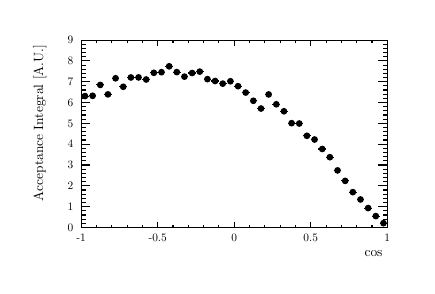
\begin{tikzpicture}
\pgfdeclareplotmark{cross} {
\pgfpathmoveto{\pgfpoint{-0.3\pgfplotmarksize}{\pgfplotmarksize}}
\pgfpathlineto{\pgfpoint{+0.3\pgfplotmarksize}{\pgfplotmarksize}}
\pgfpathlineto{\pgfpoint{+0.3\pgfplotmarksize}{0.3\pgfplotmarksize}}
\pgfpathlineto{\pgfpoint{+1\pgfplotmarksize}{0.3\pgfplotmarksize}}
\pgfpathlineto{\pgfpoint{+1\pgfplotmarksize}{-0.3\pgfplotmarksize}}
\pgfpathlineto{\pgfpoint{+0.3\pgfplotmarksize}{-0.3\pgfplotmarksize}}
\pgfpathlineto{\pgfpoint{+0.3\pgfplotmarksize}{-1.\pgfplotmarksize}}
\pgfpathlineto{\pgfpoint{-0.3\pgfplotmarksize}{-1.\pgfplotmarksize}}
\pgfpathlineto{\pgfpoint{-0.3\pgfplotmarksize}{-0.3\pgfplotmarksize}}
\pgfpathlineto{\pgfpoint{-1.\pgfplotmarksize}{-0.3\pgfplotmarksize}}
\pgfpathlineto{\pgfpoint{-1.\pgfplotmarksize}{0.3\pgfplotmarksize}}
\pgfpathlineto{\pgfpoint{-0.3\pgfplotmarksize}{0.3\pgfplotmarksize}}
\pgfpathclose
\pgfusepathqstroke
}
\pgfdeclareplotmark{cross*} {
\pgfpathmoveto{\pgfpoint{-0.3\pgfplotmarksize}{\pgfplotmarksize}}
\pgfpathlineto{\pgfpoint{+0.3\pgfplotmarksize}{\pgfplotmarksize}}
\pgfpathlineto{\pgfpoint{+0.3\pgfplotmarksize}{0.3\pgfplotmarksize}}
\pgfpathlineto{\pgfpoint{+1\pgfplotmarksize}{0.3\pgfplotmarksize}}
\pgfpathlineto{\pgfpoint{+1\pgfplotmarksize}{-0.3\pgfplotmarksize}}
\pgfpathlineto{\pgfpoint{+0.3\pgfplotmarksize}{-0.3\pgfplotmarksize}}
\pgfpathlineto{\pgfpoint{+0.3\pgfplotmarksize}{-1.\pgfplotmarksize}}
\pgfpathlineto{\pgfpoint{-0.3\pgfplotmarksize}{-1.\pgfplotmarksize}}
\pgfpathlineto{\pgfpoint{-0.3\pgfplotmarksize}{-0.3\pgfplotmarksize}}
\pgfpathlineto{\pgfpoint{-1.\pgfplotmarksize}{-0.3\pgfplotmarksize}}
\pgfpathlineto{\pgfpoint{-1.\pgfplotmarksize}{0.3\pgfplotmarksize}}
\pgfpathlineto{\pgfpoint{-0.3\pgfplotmarksize}{0.3\pgfplotmarksize}}
\pgfpathclose
\pgfusepathqfillstroke
}
\pgfdeclareplotmark{newstar} {
\pgfpathmoveto{\pgfqpoint{0pt}{\pgfplotmarksize}}
\pgfpathlineto{\pgfqpointpolar{44}{0.5\pgfplotmarksize}}
\pgfpathlineto{\pgfqpointpolar{18}{\pgfplotmarksize}}
\pgfpathlineto{\pgfqpointpolar{-20}{0.5\pgfplotmarksize}}
\pgfpathlineto{\pgfqpointpolar{-54}{\pgfplotmarksize}}
\pgfpathlineto{\pgfqpointpolar{-90}{0.5\pgfplotmarksize}}
\pgfpathlineto{\pgfqpointpolar{234}{\pgfplotmarksize}}
\pgfpathlineto{\pgfqpointpolar{198}{0.5\pgfplotmarksize}}
\pgfpathlineto{\pgfqpointpolar{162}{\pgfplotmarksize}}
\pgfpathlineto{\pgfqpointpolar{134}{0.5\pgfplotmarksize}}
\pgfpathclose
\pgfusepathqstroke
}
\pgfdeclareplotmark{newstar*} {
\pgfpathmoveto{\pgfqpoint{0pt}{\pgfplotmarksize}}
\pgfpathlineto{\pgfqpointpolar{44}{0.5\pgfplotmarksize}}
\pgfpathlineto{\pgfqpointpolar{18}{\pgfplotmarksize}}
\pgfpathlineto{\pgfqpointpolar{-20}{0.5\pgfplotmarksize}}
\pgfpathlineto{\pgfqpointpolar{-54}{\pgfplotmarksize}}
\pgfpathlineto{\pgfqpointpolar{-90}{0.5\pgfplotmarksize}}
\pgfpathlineto{\pgfqpointpolar{234}{\pgfplotmarksize}}
\pgfpathlineto{\pgfqpointpolar{198}{0.5\pgfplotmarksize}}
\pgfpathlineto{\pgfqpointpolar{162}{\pgfplotmarksize}}
\pgfpathlineto{\pgfqpointpolar{134}{0.5\pgfplotmarksize}}
\pgfpathclose
\pgfusepathqfillstroke
}
\definecolor{c}{rgb}{1,1,1};
\draw [color=c, fill=c] (0.1,3.20034) rectangle (4.9,6.21242);
\draw [color=c, fill=c] (0.772,3.68227) rectangle (4.66,6.06181);
\definecolor{c}{rgb}{0,0,0};
\draw [c] (0.772,3.68227) -- (0.772,6.06181) -- (4.66,6.06181) -- (4.66,3.68227) -- (0.772,3.68227);
\draw [c,line width=0.4] (0.8206,5.31971) -- (0.8206,5.35066);
\draw [c,line width=0.4] (0.8206,5.35066) -- (0.8206,5.38161);
\draw [c,line width=0.4] (0.772,5.35066) -- (0.8206,5.35066);
\draw [c,line width=0.4] (0.8206,5.35066) -- (0.8692,5.35066);
\foreach \P in {(0.8206,5.35066)}{\draw[mark options={color=c,fill=c},mark size=2.402402pt,mark=*,mark size=1pt] plot coordinates {\P};}
\draw [c,line width=0.4] (0.9178,5.32307) -- (0.9178,5.35406);
\draw [c,line width=0.4] (0.9178,5.35406) -- (0.9178,5.38504);
\draw [c,line width=0.4] (0.8692,5.35406) -- (0.9178,5.35406);
\draw [c,line width=0.4] (0.9178,5.35406) -- (0.9664,5.35406);
\foreach \P in {(0.9178,5.35406)}{\draw[mark options={color=c,fill=c},mark size=2.402402pt,mark=*,mark size=1pt] plot coordinates {\P};}
\draw [c,line width=0.4] (1.015,5.46011) -- (1.015,5.49235);
\draw [c,line width=0.4] (1.015,5.49235) -- (1.015,5.52459);
\draw [c,line width=0.4] (0.9664,5.49235) -- (1.015,5.49235);
\draw [c,line width=0.4] (1.015,5.49235) -- (1.0636,5.49235);
\foreach \P in {(1.015,5.49235)}{\draw[mark options={color=c,fill=c},mark size=2.402402pt,mark=*,mark size=1pt] plot coordinates {\P};}
\draw [c,line width=0.4] (1.1122,5.34102) -- (1.1122,5.37217);
\draw [c,line width=0.4] (1.1122,5.37217) -- (1.1122,5.40332);
\draw [c,line width=0.4] (1.0636,5.37217) -- (1.1122,5.37217);
\draw [c,line width=0.4] (1.1122,5.37217) -- (1.1608,5.37217);
\foreach \P in {(1.1122,5.37217)}{\draw[mark options={color=c,fill=c},mark size=2.402402pt,mark=*,mark size=1pt] plot coordinates {\P};}
\draw [c,line width=0.4] (1.2094,5.54373) -- (1.2094,5.57671);
\draw [c,line width=0.4] (1.2094,5.57671) -- (1.2094,5.60969);
\draw [c,line width=0.4] (1.1608,5.57671) -- (1.2094,5.57671);
\draw [c,line width=0.4] (1.2094,5.57671) -- (1.258,5.57671);
\foreach \P in {(1.2094,5.57671)}{\draw[mark options={color=c,fill=c},mark size=2.402402pt,mark=*,mark size=1pt] plot coordinates {\P};}
\draw [c,line width=0.4] (1.3066,5.43649) -- (1.3066,5.46851);
\draw [c,line width=0.4] (1.3066,5.46851) -- (1.3066,5.50054);
\draw [c,line width=0.4] (1.258,5.46851) -- (1.3066,5.46851);
\draw [c,line width=0.4] (1.3066,5.46851) -- (1.3552,5.46851);
\foreach \P in {(1.3066,5.46851)}{\draw[mark options={color=c,fill=c},mark size=2.402402pt,mark=*,mark size=1pt] plot coordinates {\P};}
\draw [c,line width=0.4] (1.4038,5.55408) -- (1.4038,5.58715);
\draw [c,line width=0.4] (1.4038,5.58715) -- (1.4038,5.62022);
\draw [c,line width=0.4] (1.3552,5.58715) -- (1.4038,5.58715);
\draw [c,line width=0.4] (1.4038,5.58715) -- (1.4524,5.58715);
\foreach \P in {(1.4038,5.58715)}{\draw[mark options={color=c,fill=c},mark size=2.402402pt,mark=*,mark size=1pt] plot coordinates {\P};}
\draw [c,line width=0.4] (1.501,5.55471) -- (1.501,5.58779);
\draw [c,line width=0.4] (1.501,5.58779) -- (1.501,5.62087);
\draw [c,line width=0.4] (1.4524,5.58779) -- (1.501,5.58779);
\draw [c,line width=0.4] (1.501,5.58779) -- (1.5496,5.58779);
\foreach \P in {(1.501,5.58779)}{\draw[mark options={color=c,fill=c},mark size=2.402402pt,mark=*,mark size=1pt] plot coordinates {\P};}
\draw [c,line width=0.4] (1.5982,5.52853) -- (1.5982,5.56138);
\draw [c,line width=0.4] (1.5982,5.56138) -- (1.5982,5.59423);
\draw [c,line width=0.4] (1.5496,5.56138) -- (1.5982,5.56138);
\draw [c,line width=0.4] (1.5982,5.56138) -- (1.6468,5.56138);
\foreach \P in {(1.5982,5.56138)}{\draw[mark options={color=c,fill=c},mark size=2.402402pt,mark=*,mark size=1pt] plot coordinates {\P};}
\draw [c,line width=0.4] (1.6954,5.61241) -- (1.6954,5.64599);
\draw [c,line width=0.4] (1.6954,5.64599) -- (1.6954,5.67957);
\draw [c,line width=0.4] (1.6468,5.64599) -- (1.6954,5.64599);
\draw [c,line width=0.4] (1.6954,5.64599) -- (1.744,5.64599);
\foreach \P in {(1.6954,5.64599)}{\draw[mark options={color=c,fill=c},mark size=2.402402pt,mark=*,mark size=1pt] plot coordinates {\P};}
\draw [c,line width=0.4] (1.7926,5.62027) -- (1.7926,5.65391);
\draw [c,line width=0.4] (1.7926,5.65391) -- (1.7926,5.68756);
\draw [c,line width=0.4] (1.744,5.65391) -- (1.7926,5.65391);
\draw [c,line width=0.4] (1.7926,5.65391) -- (1.8412,5.65391);
\foreach \P in {(1.7926,5.65391)}{\draw[mark options={color=c,fill=c},mark size=2.402402pt,mark=*,mark size=1pt] plot coordinates {\P};}
\draw [c,line width=0.4] (1.8898,5.69449) -- (1.8898,5.72877);
\draw [c,line width=0.4] (1.8898,5.72877) -- (1.8898,5.76305);
\draw [c,line width=0.4] (1.8412,5.72877) -- (1.8898,5.72877);
\draw [c,line width=0.4] (1.8898,5.72877) -- (1.9384,5.72877);
\foreach \P in {(1.8898,5.72877)}{\draw[mark options={color=c,fill=c},mark size=2.402402pt,mark=*,mark size=1pt] plot coordinates {\P};}
\draw [c,line width=0.4] (1.987,5.62135) -- (1.987,5.655);
\draw [c,line width=0.4] (1.987,5.655) -- (1.987,5.68866);
\draw [c,line width=0.4] (1.9384,5.655) -- (1.987,5.655);
\draw [c,line width=0.4] (1.987,5.655) -- (2.0356,5.655);
\foreach \P in {(1.987,5.655)}{\draw[mark options={color=c,fill=c},mark size=2.402402pt,mark=*,mark size=1pt] plot coordinates {\P};}
\draw [c,line width=0.4] (2.0842,5.56435) -- (2.0842,5.59751);
\draw [c,line width=0.4] (2.0842,5.59751) -- (2.0842,5.63068);
\draw [c,line width=0.4] (2.0356,5.59751) -- (2.0842,5.59751);
\draw [c,line width=0.4] (2.0842,5.59751) -- (2.1328,5.59751);
\foreach \P in {(2.0842,5.59751)}{\draw[mark options={color=c,fill=c},mark size=2.402402pt,mark=*,mark size=1pt] plot coordinates {\P};}
\draw [c,line width=0.4] (2.1814,5.60978) -- (2.1814,5.64333);
\draw [c,line width=0.4] (2.1814,5.64333) -- (2.1814,5.67689);
\draw [c,line width=0.4] (2.1328,5.64333) -- (2.1814,5.64333);
\draw [c,line width=0.4] (2.1814,5.64333) -- (2.23,5.64333);
\foreach \P in {(2.1814,5.64333)}{\draw[mark options={color=c,fill=c},mark size=2.402402pt,mark=*,mark size=1pt] plot coordinates {\P};}
\draw [c,line width=0.4] (2.2786,5.62741) -- (2.2786,5.66112);
\draw [c,line width=0.4] (2.2786,5.66112) -- (2.2786,5.69482);
\draw [c,line width=0.4] (2.23,5.66112) -- (2.2786,5.66112);
\draw [c,line width=0.4] (2.2786,5.66112) -- (2.3272,5.66112);
\foreach \P in {(2.2786,5.66112)}{\draw[mark options={color=c,fill=c},mark size=2.402402pt,mark=*,mark size=1pt] plot coordinates {\P};}
\draw [c,line width=0.4] (2.3758,5.53291) -- (2.3758,5.5658);
\draw [c,line width=0.4] (2.3758,5.5658) -- (2.3758,5.59869);
\draw [c,line width=0.4] (2.3272,5.5658) -- (2.3758,5.5658);
\draw [c,line width=0.4] (2.3758,5.5658) -- (2.4244,5.5658);
\foreach \P in {(2.3758,5.5658)}{\draw[mark options={color=c,fill=c},mark size=2.402402pt,mark=*,mark size=1pt] plot coordinates {\P};}
\draw [c,line width=0.4] (2.473,5.50916) -- (2.473,5.54184);
\draw [c,line width=0.4] (2.473,5.54184) -- (2.473,5.57451);
\draw [c,line width=0.4] (2.4244,5.54184) -- (2.473,5.54184);
\draw [c,line width=0.4] (2.473,5.54184) -- (2.5216,5.54184);
\foreach \P in {(2.473,5.54184)}{\draw[mark options={color=c,fill=c},mark size=2.402402pt,mark=*,mark size=1pt] plot coordinates {\P};}
\draw [c,line width=0.4] (2.5702,5.47631) -- (2.5702,5.50869);
\draw [c,line width=0.4] (2.5702,5.50869) -- (2.5702,5.54107);
\draw [c,line width=0.4] (2.5216,5.50869) -- (2.5702,5.50869);
\draw [c,line width=0.4] (2.5702,5.50869) -- (2.6188,5.50869);
\foreach \P in {(2.5702,5.50869)}{\draw[mark options={color=c,fill=c},mark size=2.402402pt,mark=*,mark size=1pt] plot coordinates {\P};}
\draw [c,line width=0.4] (2.6674,5.50627) -- (2.6674,5.53892);
\draw [c,line width=0.4] (2.6674,5.53892) -- (2.6674,5.57157);
\draw [c,line width=0.4] (2.6188,5.53892) -- (2.6674,5.53892);
\draw [c,line width=0.4] (2.6674,5.53892) -- (2.716,5.53892);
\foreach \P in {(2.6674,5.53892)}{\draw[mark options={color=c,fill=c},mark size=2.402402pt,mark=*,mark size=1pt] plot coordinates {\P};}
\draw [c,line width=0.4] (2.7646,5.44424) -- (2.7646,5.47634);
\draw [c,line width=0.4] (2.7646,5.47634) -- (2.7646,5.50843);
\draw [c,line width=0.4] (2.716,5.47634) -- (2.7646,5.47634);
\draw [c,line width=0.4] (2.7646,5.47634) -- (2.8132,5.47634);
\foreach \P in {(2.7646,5.47634)}{\draw[mark options={color=c,fill=c},mark size=2.402402pt,mark=*,mark size=1pt] plot coordinates {\P};}
\draw [c,line width=0.4] (2.8618,5.36421) -- (2.8618,5.39557);
\draw [c,line width=0.4] (2.8618,5.39557) -- (2.8618,5.42694);
\draw [c,line width=0.4] (2.8132,5.39557) -- (2.8618,5.39557);
\draw [c,line width=0.4] (2.8618,5.39557) -- (2.9104,5.39557);
\foreach \P in {(2.8618,5.39557)}{\draw[mark options={color=c,fill=c},mark size=2.402402pt,mark=*,mark size=1pt] plot coordinates {\P};}
\draw [c,line width=0.4] (2.959,5.26073) -- (2.959,5.29112);
\draw [c,line width=0.4] (2.959,5.29112) -- (2.959,5.32151);
\draw [c,line width=0.4] (2.9104,5.29112) -- (2.959,5.29112);
\draw [c,line width=0.4] (2.959,5.29112) -- (3.0076,5.29112);
\foreach \P in {(2.959,5.29112)}{\draw[mark options={color=c,fill=c},mark size=2.402402pt,mark=*,mark size=1pt] plot coordinates {\P};}
\draw [c,line width=0.4] (3.0562,5.16296) -- (3.0562,5.1924);
\draw [c,line width=0.4] (3.0562,5.1924) -- (3.0562,5.22185);
\draw [c,line width=0.4] (3.0076,5.1924) -- (3.0562,5.1924);
\draw [c,line width=0.4] (3.0562,5.1924) -- (3.1048,5.1924);
\foreach \P in {(3.0562,5.1924)}{\draw[mark options={color=c,fill=c},mark size=2.402402pt,mark=*,mark size=1pt] plot coordinates {\P};}
\draw [c,line width=0.4] (3.1534,5.3403) -- (3.1534,5.37145);
\draw [c,line width=0.4] (3.1534,5.37145) -- (3.1534,5.40259);
\draw [c,line width=0.4] (3.1048,5.37145) -- (3.1534,5.37145);
\draw [c,line width=0.4] (3.1534,5.37145) -- (3.202,5.37145);
\foreach \P in {(3.1534,5.37145)}{\draw[mark options={color=c,fill=c},mark size=2.402402pt,mark=*,mark size=1pt] plot coordinates {\P};}
\draw [c,line width=0.4] (3.2506,5.21647) -- (3.2506,5.24644);
\draw [c,line width=0.4] (3.2506,5.24644) -- (3.2506,5.27641);
\draw [c,line width=0.4] (3.202,5.24644) -- (3.2506,5.24644);
\draw [c,line width=0.4] (3.2506,5.24644) -- (3.2992,5.24644);
\foreach \P in {(3.2506,5.24644)}{\draw[mark options={color=c,fill=c},mark size=2.402402pt,mark=*,mark size=1pt] plot coordinates {\P};}
\draw [c,line width=0.4] (3.3478,5.12858) -- (3.3478,5.15768);
\draw [c,line width=0.4] (3.3478,5.15768) -- (3.3478,5.18679);
\draw [c,line width=0.4] (3.2992,5.15768) -- (3.3478,5.15768);
\draw [c,line width=0.4] (3.3478,5.15768) -- (3.3964,5.15768);
\foreach \P in {(3.3478,5.15768)}{\draw[mark options={color=c,fill=c},mark size=2.402402pt,mark=*,mark size=1pt] plot coordinates {\P};}
\draw [c,line width=0.4] (3.445,4.97916) -- (3.445,5.00674);
\draw [c,line width=0.4] (3.445,5.00674) -- (3.445,5.03432);
\draw [c,line width=0.4] (3.3964,5.00674) -- (3.445,5.00674);
\draw [c,line width=0.4] (3.445,5.00674) -- (3.4936,5.00674);
\foreach \P in {(3.445,5.00674)}{\draw[mark options={color=c,fill=c},mark size=2.402402pt,mark=*,mark size=1pt] plot coordinates {\P};}
\draw [c,line width=0.4] (3.5422,4.97466) -- (3.5422,5.00219);
\draw [c,line width=0.4] (3.5422,5.00219) -- (3.5422,5.02972);
\draw [c,line width=0.4] (3.4936,5.00219) -- (3.5422,5.00219);
\draw [c,line width=0.4] (3.5422,5.00219) -- (3.5908,5.00219);
\foreach \P in {(3.5422,5.00219)}{\draw[mark options={color=c,fill=c},mark size=2.402402pt,mark=*,mark size=1pt] plot coordinates {\P};}
\draw [c,line width=0.4] (3.6394,4.8205) -- (3.6394,4.84636);
\draw [c,line width=0.4] (3.6394,4.84636) -- (3.6394,4.87221);
\draw [c,line width=0.4] (3.5908,4.84636) -- (3.6394,4.84636);
\draw [c,line width=0.4] (3.6394,4.84636) -- (3.688,4.84636);
\foreach \P in {(3.6394,4.84636)}{\draw[mark options={color=c,fill=c},mark size=2.402402pt,mark=*,mark size=1pt] plot coordinates {\P};}
\draw [c,line width=0.4] (3.7366,4.77361) -- (3.7366,4.79893);
\draw [c,line width=0.4] (3.7366,4.79893) -- (3.7366,4.82426);
\draw [c,line width=0.4] (3.688,4.79893) -- (3.7366,4.79893);
\draw [c,line width=0.4] (3.7366,4.79893) -- (3.7852,4.79893);
\foreach \P in {(3.7366,4.79893)}{\draw[mark options={color=c,fill=c},mark size=2.402402pt,mark=*,mark size=1pt] plot coordinates {\P};}
\draw [c,line width=0.4] (3.8338,4.65497) -- (3.8338,4.67889);
\draw [c,line width=0.4] (3.8338,4.67889) -- (3.8338,4.70281);
\draw [c,line width=0.4] (3.7852,4.67889) -- (3.8338,4.67889);
\draw [c,line width=0.4] (3.8338,4.67889) -- (3.8824,4.67889);
\foreach \P in {(3.8338,4.67889)}{\draw[mark options={color=c,fill=c},mark size=2.402402pt,mark=*,mark size=1pt] plot coordinates {\P};}
\draw [c,line width=0.4] (3.931,4.55195) -- (3.931,4.57459);
\draw [c,line width=0.4] (3.931,4.57459) -- (3.931,4.59723);
\draw [c,line width=0.4] (3.8824,4.57459) -- (3.931,4.57459);
\draw [c,line width=0.4] (3.931,4.57459) -- (3.9796,4.57459);
\foreach \P in {(3.931,4.57459)}{\draw[mark options={color=c,fill=c},mark size=2.402402pt,mark=*,mark size=1pt] plot coordinates {\P};}
\draw [c,line width=0.4] (4.0282,4.38631) -- (4.0282,4.4067);
\draw [c,line width=0.4] (4.0282,4.4067) -- (4.0282,4.4271);
\draw [c,line width=0.4] (3.9796,4.4067) -- (4.0282,4.4067);
\draw [c,line width=0.4] (4.0282,4.4067) -- (4.0768,4.4067);
\foreach \P in {(4.0282,4.4067)}{\draw[mark options={color=c,fill=c},mark size=2.402402pt,mark=*,mark size=1pt] plot coordinates {\P};}
\draw [c,line width=0.4] (4.1254,4.25522) -- (4.1254,4.27365);
\draw [c,line width=0.4] (4.1254,4.27365) -- (4.1254,4.29208);
\draw [c,line width=0.4] (4.0768,4.27365) -- (4.1254,4.27365);
\draw [c,line width=0.4] (4.1254,4.27365) -- (4.174,4.27365);
\foreach \P in {(4.1254,4.27365)}{\draw[mark options={color=c,fill=c},mark size=2.402402pt,mark=*,mark size=1pt] plot coordinates {\P};}
\draw [c,line width=0.4] (4.2226,4.11469) -- (4.2226,4.13073);
\draw [c,line width=0.4] (4.2226,4.13073) -- (4.2226,4.14678);
\draw [c,line width=0.4] (4.174,4.13073) -- (4.2226,4.13073);
\draw [c,line width=0.4] (4.2226,4.13073) -- (4.2712,4.13073);
\foreach \P in {(4.2226,4.13073)}{\draw[mark options={color=c,fill=c},mark size=2.402402pt,mark=*,mark size=1pt] plot coordinates {\P};}
\draw [c,line width=0.4] (4.3198,4.0234) -- (4.3198,4.03768);
\draw [c,line width=0.4] (4.3198,4.03768) -- (4.3198,4.05197);
\draw [c,line width=0.4] (4.2712,4.03768) -- (4.3198,4.03768);
\draw [c,line width=0.4] (4.3198,4.03768) -- (4.3684,4.03768);
\foreach \P in {(4.3198,4.03768)}{\draw[mark options={color=c,fill=c},mark size=2.402402pt,mark=*,mark size=1pt] plot coordinates {\P};}
\draw [c,line width=0.4] (4.417,3.9165) -- (4.417,3.92838);
\draw [c,line width=0.4] (4.417,3.92838) -- (4.417,3.94027);
\draw [c,line width=0.4] (4.3684,3.92838) -- (4.417,3.92838);
\draw [c,line width=0.4] (4.417,3.92838) -- (4.4656,3.92838);
\foreach \P in {(4.417,3.92838)}{\draw[mark options={color=c,fill=c},mark size=2.402402pt,mark=*,mark size=1pt] plot coordinates {\P};}
\draw [c,line width=0.4] (4.5142,3.81734) -- (4.5142,3.82644);
\draw [c,line width=0.4] (4.5142,3.82644) -- (4.5142,3.83554);
\draw [c,line width=0.4] (4.4656,3.82644) -- (4.5142,3.82644);
\draw [c,line width=0.4] (4.5142,3.82644) -- (4.5628,3.82644);
\foreach \P in {(4.5142,3.82644)}{\draw[mark options={color=c,fill=c},mark size=2.402402pt,mark=*,mark size=1pt] plot coordinates {\P};}
\draw [c,line width=0.4] (4.6114,3.7311) -- (4.6114,3.73669);
\draw [c,line width=0.4] (4.6114,3.73669) -- (4.6114,3.74227);
\draw [c,line width=0.4] (4.5628,3.73669) -- (4.6114,3.73669);
\draw [c,line width=0.4] (4.6114,3.73669) -- (4.66,3.73669);
\foreach \P in {(4.6114,3.73669)}{\draw[mark options={color=c,fill=c},mark size=2.402402pt,mark=*,mark size=1pt] plot coordinates {\P};}
\draw [c,line width=0.4] (0.772,3.68227) -- (4.66,3.68227);
\draw [anchor= east] (4.66,3.35263) node[scale=0.485847, rotate=0]{$\cos\thetaK$};
\draw [c,line width=0.4] (0.772,3.75546) -- (0.772,3.68227);
\draw [c,line width=0.4] (0.9664,3.71887) -- (0.9664,3.68227);
\draw [c,line width=0.4] (1.1608,3.71887) -- (1.1608,3.68227);
\draw [c,line width=0.4] (1.3552,3.71887) -- (1.3552,3.68227);
\draw [c,line width=0.4] (1.5496,3.71887) -- (1.5496,3.68227);
\draw [c,line width=0.4] (1.744,3.75546) -- (1.744,3.68227);
\draw [c,line width=0.4] (1.9384,3.71887) -- (1.9384,3.68227);
\draw [c,line width=0.4] (2.1328,3.71887) -- (2.1328,3.68227);
\draw [c,line width=0.4] (2.3272,3.71887) -- (2.3272,3.68227);
\draw [c,line width=0.4] (2.5216,3.71887) -- (2.5216,3.68227);
\draw [c,line width=0.4] (2.716,3.75546) -- (2.716,3.68227);
\draw [c,line width=0.4] (2.9104,3.71887) -- (2.9104,3.68227);
\draw [c,line width=0.4] (3.1048,3.71887) -- (3.1048,3.68227);
\draw [c,line width=0.4] (3.2992,3.71887) -- (3.2992,3.68227);
\draw [c,line width=0.4] (3.4936,3.71887) -- (3.4936,3.68227);
\draw [c,line width=0.4] (3.688,3.75546) -- (3.688,3.68227);
\draw [c,line width=0.4] (3.8824,3.71887) -- (3.8824,3.68227);
\draw [c,line width=0.4] (4.0768,3.71887) -- (4.0768,3.68227);
\draw [c,line width=0.4] (4.2712,3.71887) -- (4.2712,3.68227);
\draw [c,line width=0.4] (4.4656,3.71887) -- (4.4656,3.68227);
\draw [c,line width=0.4] (4.66,3.75546) -- (4.66,3.68227);
\draw [anchor=base] (0.772,3.50757) node[scale=0.411101, rotate=0]{-1};
\draw [anchor=base] (1.744,3.50757) node[scale=0.411101, rotate=0]{-0.5};
\draw [anchor=base] (2.716,3.50757) node[scale=0.411101, rotate=0]{0};
\draw [anchor=base] (3.688,3.50757) node[scale=0.411101, rotate=0]{0.5};
\draw [anchor=base] (4.66,3.50757) node[scale=0.411101, rotate=0]{1};
\draw [c,line width=0.4] (0.772,6.06181) -- (4.66,6.06181);
\draw [c,line width=0.4] (0.772,5.98862) -- (0.772,6.06181);
\draw [c,line width=0.4] (0.9664,6.02522) -- (0.9664,6.06181);
\draw [c,line width=0.4] (1.1608,6.02522) -- (1.1608,6.06181);
\draw [c,line width=0.4] (1.3552,6.02522) -- (1.3552,6.06181);
\draw [c,line width=0.4] (1.5496,6.02522) -- (1.5496,6.06181);
\draw [c,line width=0.4] (1.744,5.98862) -- (1.744,6.06181);
\draw [c,line width=0.4] (1.9384,6.02522) -- (1.9384,6.06181);
\draw [c,line width=0.4] (2.1328,6.02522) -- (2.1328,6.06181);
\draw [c,line width=0.4] (2.3272,6.02522) -- (2.3272,6.06181);
\draw [c,line width=0.4] (2.5216,6.02522) -- (2.5216,6.06181);
\draw [c,line width=0.4] (2.716,5.98862) -- (2.716,6.06181);
\draw [c,line width=0.4] (2.9104,6.02522) -- (2.9104,6.06181);
\draw [c,line width=0.4] (3.1048,6.02522) -- (3.1048,6.06181);
\draw [c,line width=0.4] (3.2992,6.02522) -- (3.2992,6.06181);
\draw [c,line width=0.4] (3.4936,6.02522) -- (3.4936,6.06181);
\draw [c,line width=0.4] (3.688,5.98862) -- (3.688,6.06181);
\draw [c,line width=0.4] (3.8824,6.02522) -- (3.8824,6.06181);
\draw [c,line width=0.4] (4.0768,6.02522) -- (4.0768,6.06181);
\draw [c,line width=0.4] (4.2712,6.02522) -- (4.2712,6.06181);
\draw [c,line width=0.4] (4.4656,6.02522) -- (4.4656,6.06181);
\draw [c,line width=0.4] (4.66,5.98862) -- (4.66,6.06181);
\draw [c,line width=0.4] (0.772,3.68227) -- (0.772,6.06181);
\draw [anchor= east] (0.246688,6.06181) node[scale=0.485847, rotate=90]{Acceptance Integral [A.U.]};
\draw [c,line width=0.4] (0.88576,3.68227) -- (0.772,3.68227);
\draw [c,line width=0.4] (0.82888,3.73515) -- (0.772,3.73515);
\draw [c,line width=0.4] (0.82888,3.78803) -- (0.772,3.78803);
\draw [c,line width=0.4] (0.82888,3.8409) -- (0.772,3.8409);
\draw [c,line width=0.4] (0.82888,3.89378) -- (0.772,3.89378);
\draw [c,line width=0.4] (0.88576,3.94666) -- (0.772,3.94666);
\draw [c,line width=0.4] (0.82888,3.99954) -- (0.772,3.99954);
\draw [c,line width=0.4] (0.82888,4.05242) -- (0.772,4.05242);
\draw [c,line width=0.4] (0.82888,4.1053) -- (0.772,4.1053);
\draw [c,line width=0.4] (0.82888,4.15818) -- (0.772,4.15818);
\draw [c,line width=0.4] (0.88576,4.21106) -- (0.772,4.21106);
\draw [c,line width=0.4] (0.82888,4.26393) -- (0.772,4.26393);
\draw [c,line width=0.4] (0.82888,4.31681) -- (0.772,4.31681);
\draw [c,line width=0.4] (0.82888,4.36969) -- (0.772,4.36969);
\draw [c,line width=0.4] (0.82888,4.42257) -- (0.772,4.42257);
\draw [c,line width=0.4] (0.88576,4.47545) -- (0.772,4.47545);
\draw [c,line width=0.4] (0.82888,4.52833) -- (0.772,4.52833);
\draw [c,line width=0.4] (0.82888,4.58121) -- (0.772,4.58121);
\draw [c,line width=0.4] (0.82888,4.63409) -- (0.772,4.63409);
\draw [c,line width=0.4] (0.82888,4.68696) -- (0.772,4.68696);
\draw [c,line width=0.4] (0.88576,4.73984) -- (0.772,4.73984);
\draw [c,line width=0.4] (0.82888,4.79272) -- (0.772,4.79272);
\draw [c,line width=0.4] (0.82888,4.8456) -- (0.772,4.8456);
\draw [c,line width=0.4] (0.82888,4.89848) -- (0.772,4.89848);
\draw [c,line width=0.4] (0.82888,4.95136) -- (0.772,4.95136);
\draw [c,line width=0.4] (0.88576,5.00424) -- (0.772,5.00424);
\draw [c,line width=0.4] (0.82888,5.05712) -- (0.772,5.05712);
\draw [c,line width=0.4] (0.82888,5.10999) -- (0.772,5.10999);
\draw [c,line width=0.4] (0.82888,5.16287) -- (0.772,5.16287);
\draw [c,line width=0.4] (0.82888,5.21575) -- (0.772,5.21575);
\draw [c,line width=0.4] (0.88576,5.26863) -- (0.772,5.26863);
\draw [c,line width=0.4] (0.82888,5.32151) -- (0.772,5.32151);
\draw [c,line width=0.4] (0.82888,5.37439) -- (0.772,5.37439);
\draw [c,line width=0.4] (0.82888,5.42727) -- (0.772,5.42727);
\draw [c,line width=0.4] (0.82888,5.48015) -- (0.772,5.48015);
\draw [c,line width=0.4] (0.88576,5.53302) -- (0.772,5.53302);
\draw [c,line width=0.4] (0.82888,5.5859) -- (0.772,5.5859);
\draw [c,line width=0.4] (0.82888,5.63878) -- (0.772,5.63878);
\draw [c,line width=0.4] (0.82888,5.69166) -- (0.772,5.69166);
\draw [c,line width=0.4] (0.82888,5.74454) -- (0.772,5.74454);
\draw [c,line width=0.4] (0.88576,5.79742) -- (0.772,5.79742);
\draw [c,line width=0.4] (0.82888,5.8503) -- (0.772,5.8503);
\draw [c,line width=0.4] (0.82888,5.90318) -- (0.772,5.90318);
\draw [c,line width=0.4] (0.82888,5.95605) -- (0.772,5.95605);
\draw [c,line width=0.4] (0.82888,6.00893) -- (0.772,6.00893);
\draw [c,line width=0.4] (0.88576,6.06181) -- (0.772,6.06181);
\draw [anchor= east] (0.724,3.68227) node[scale=0.411101, rotate=0]{0};
\draw [anchor= east] (0.724,3.94666) node[scale=0.411101, rotate=0]{1};
\draw [anchor= east] (0.724,4.21106) node[scale=0.411101, rotate=0]{2};
\draw [anchor= east] (0.724,4.47545) node[scale=0.411101, rotate=0]{3};
\draw [anchor= east] (0.724,4.73984) node[scale=0.411101, rotate=0]{4};
\draw [anchor= east] (0.724,5.00424) node[scale=0.411101, rotate=0]{5};
\draw [anchor= east] (0.724,5.26863) node[scale=0.411101, rotate=0]{6};
\draw [anchor= east] (0.724,5.53302) node[scale=0.411101, rotate=0]{7};
\draw [anchor= east] (0.724,5.79742) node[scale=0.411101, rotate=0]{8};
\draw [anchor= east] (0.724,6.06181) node[scale=0.411101, rotate=0]{9};
\draw [c,line width=0.4] (4.66,3.68227) -- (4.66,6.06181);
\draw [c,line width=0.4] (4.54624,3.68227) -- (4.66,3.68227);
\draw [c,line width=0.4] (4.60312,3.73515) -- (4.66,3.73515);
\draw [c,line width=0.4] (4.60312,3.78803) -- (4.66,3.78803);
\draw [c,line width=0.4] (4.60312,3.8409) -- (4.66,3.8409);
\draw [c,line width=0.4] (4.60312,3.89378) -- (4.66,3.89378);
\draw [c,line width=0.4] (4.54624,3.94666) -- (4.66,3.94666);
\draw [c,line width=0.4] (4.60312,3.99954) -- (4.66,3.99954);
\draw [c,line width=0.4] (4.60312,4.05242) -- (4.66,4.05242);
\draw [c,line width=0.4] (4.60312,4.1053) -- (4.66,4.1053);
\draw [c,line width=0.4] (4.60312,4.15818) -- (4.66,4.15818);
\draw [c,line width=0.4] (4.54624,4.21106) -- (4.66,4.21106);
\draw [c,line width=0.4] (4.60312,4.26393) -- (4.66,4.26393);
\draw [c,line width=0.4] (4.60312,4.31681) -- (4.66,4.31681);
\draw [c,line width=0.4] (4.60312,4.36969) -- (4.66,4.36969);
\draw [c,line width=0.4] (4.60312,4.42257) -- (4.66,4.42257);
\draw [c,line width=0.4] (4.54624,4.47545) -- (4.66,4.47545);
\draw [c,line width=0.4] (4.60312,4.52833) -- (4.66,4.52833);
\draw [c,line width=0.4] (4.60312,4.58121) -- (4.66,4.58121);
\draw [c,line width=0.4] (4.60312,4.63409) -- (4.66,4.63409);
\draw [c,line width=0.4] (4.60312,4.68696) -- (4.66,4.68696);
\draw [c,line width=0.4] (4.54624,4.73984) -- (4.66,4.73984);
\draw [c,line width=0.4] (4.60312,4.79272) -- (4.66,4.79272);
\draw [c,line width=0.4] (4.60312,4.8456) -- (4.66,4.8456);
\draw [c,line width=0.4] (4.60312,4.89848) -- (4.66,4.89848);
\draw [c,line width=0.4] (4.60312,4.95136) -- (4.66,4.95136);
\draw [c,line width=0.4] (4.54624,5.00424) -- (4.66,5.00424);
\draw [c,line width=0.4] (4.60312,5.05712) -- (4.66,5.05712);
\draw [c,line width=0.4] (4.60312,5.10999) -- (4.66,5.10999);
\draw [c,line width=0.4] (4.60312,5.16287) -- (4.66,5.16287);
\draw [c,line width=0.4] (4.60312,5.21575) -- (4.66,5.21575);
\draw [c,line width=0.4] (4.54624,5.26863) -- (4.66,5.26863);
\draw [c,line width=0.4] (4.60312,5.32151) -- (4.66,5.32151);
\draw [c,line width=0.4] (4.60312,5.37439) -- (4.66,5.37439);
\draw [c,line width=0.4] (4.60312,5.42727) -- (4.66,5.42727);
\draw [c,line width=0.4] (4.60312,5.48015) -- (4.66,5.48015);
\draw [c,line width=0.4] (4.54624,5.53302) -- (4.66,5.53302);
\draw [c,line width=0.4] (4.60312,5.5859) -- (4.66,5.5859);
\draw [c,line width=0.4] (4.60312,5.63878) -- (4.66,5.63878);
\draw [c,line width=0.4] (4.60312,5.69166) -- (4.66,5.69166);
\draw [c,line width=0.4] (4.60312,5.74454) -- (4.66,5.74454);
\draw [c,line width=0.4] (4.54624,5.79742) -- (4.66,5.79742);
\draw [c,line width=0.4] (4.60312,5.8503) -- (4.66,5.8503);
\draw [c,line width=0.4] (4.60312,5.90318) -- (4.66,5.90318);
\draw [c,line width=0.4] (4.60312,5.95605) -- (4.66,5.95605);
\draw [c,line width=0.4] (4.60312,6.00893) -- (4.66,6.00893);
\draw [c,line width=0.4] (4.54624,6.06181) -- (4.66,6.06181);
\end{tikzpicture}
}
    \caption{}
    \label{angAcc_ctk}
  \end{subfigure}%
  \hfill%
  \begin{subfigure}{0.49\textwidth}
    \tikzsetnextfilename{eff_data_helcosthetaL_allKaons_binall}
    \scalebox{1.3}{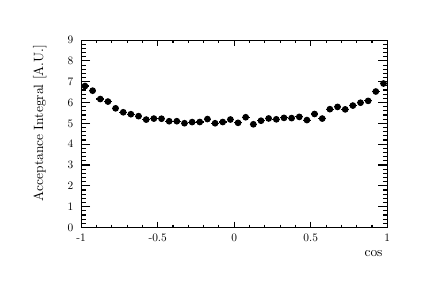
\begin{tikzpicture}
\pgfdeclareplotmark{cross} {
\pgfpathmoveto{\pgfpoint{-0.3\pgfplotmarksize}{\pgfplotmarksize}}
\pgfpathlineto{\pgfpoint{+0.3\pgfplotmarksize}{\pgfplotmarksize}}
\pgfpathlineto{\pgfpoint{+0.3\pgfplotmarksize}{0.3\pgfplotmarksize}}
\pgfpathlineto{\pgfpoint{+1\pgfplotmarksize}{0.3\pgfplotmarksize}}
\pgfpathlineto{\pgfpoint{+1\pgfplotmarksize}{-0.3\pgfplotmarksize}}
\pgfpathlineto{\pgfpoint{+0.3\pgfplotmarksize}{-0.3\pgfplotmarksize}}
\pgfpathlineto{\pgfpoint{+0.3\pgfplotmarksize}{-1.\pgfplotmarksize}}
\pgfpathlineto{\pgfpoint{-0.3\pgfplotmarksize}{-1.\pgfplotmarksize}}
\pgfpathlineto{\pgfpoint{-0.3\pgfplotmarksize}{-0.3\pgfplotmarksize}}
\pgfpathlineto{\pgfpoint{-1.\pgfplotmarksize}{-0.3\pgfplotmarksize}}
\pgfpathlineto{\pgfpoint{-1.\pgfplotmarksize}{0.3\pgfplotmarksize}}
\pgfpathlineto{\pgfpoint{-0.3\pgfplotmarksize}{0.3\pgfplotmarksize}}
\pgfpathclose
\pgfusepathqstroke
}
\pgfdeclareplotmark{cross*} {
\pgfpathmoveto{\pgfpoint{-0.3\pgfplotmarksize}{\pgfplotmarksize}}
\pgfpathlineto{\pgfpoint{+0.3\pgfplotmarksize}{\pgfplotmarksize}}
\pgfpathlineto{\pgfpoint{+0.3\pgfplotmarksize}{0.3\pgfplotmarksize}}
\pgfpathlineto{\pgfpoint{+1\pgfplotmarksize}{0.3\pgfplotmarksize}}
\pgfpathlineto{\pgfpoint{+1\pgfplotmarksize}{-0.3\pgfplotmarksize}}
\pgfpathlineto{\pgfpoint{+0.3\pgfplotmarksize}{-0.3\pgfplotmarksize}}
\pgfpathlineto{\pgfpoint{+0.3\pgfplotmarksize}{-1.\pgfplotmarksize}}
\pgfpathlineto{\pgfpoint{-0.3\pgfplotmarksize}{-1.\pgfplotmarksize}}
\pgfpathlineto{\pgfpoint{-0.3\pgfplotmarksize}{-0.3\pgfplotmarksize}}
\pgfpathlineto{\pgfpoint{-1.\pgfplotmarksize}{-0.3\pgfplotmarksize}}
\pgfpathlineto{\pgfpoint{-1.\pgfplotmarksize}{0.3\pgfplotmarksize}}
\pgfpathlineto{\pgfpoint{-0.3\pgfplotmarksize}{0.3\pgfplotmarksize}}
\pgfpathclose
\pgfusepathqfillstroke
}
\pgfdeclareplotmark{newstar} {
\pgfpathmoveto{\pgfqpoint{0pt}{\pgfplotmarksize}}
\pgfpathlineto{\pgfqpointpolar{44}{0.5\pgfplotmarksize}}
\pgfpathlineto{\pgfqpointpolar{18}{\pgfplotmarksize}}
\pgfpathlineto{\pgfqpointpolar{-20}{0.5\pgfplotmarksize}}
\pgfpathlineto{\pgfqpointpolar{-54}{\pgfplotmarksize}}
\pgfpathlineto{\pgfqpointpolar{-90}{0.5\pgfplotmarksize}}
\pgfpathlineto{\pgfqpointpolar{234}{\pgfplotmarksize}}
\pgfpathlineto{\pgfqpointpolar{198}{0.5\pgfplotmarksize}}
\pgfpathlineto{\pgfqpointpolar{162}{\pgfplotmarksize}}
\pgfpathlineto{\pgfqpointpolar{134}{0.5\pgfplotmarksize}}
\pgfpathclose
\pgfusepathqstroke
}
\pgfdeclareplotmark{newstar*} {
\pgfpathmoveto{\pgfqpoint{0pt}{\pgfplotmarksize}}
\pgfpathlineto{\pgfqpointpolar{44}{0.5\pgfplotmarksize}}
\pgfpathlineto{\pgfqpointpolar{18}{\pgfplotmarksize}}
\pgfpathlineto{\pgfqpointpolar{-20}{0.5\pgfplotmarksize}}
\pgfpathlineto{\pgfqpointpolar{-54}{\pgfplotmarksize}}
\pgfpathlineto{\pgfqpointpolar{-90}{0.5\pgfplotmarksize}}
\pgfpathlineto{\pgfqpointpolar{234}{\pgfplotmarksize}}
\pgfpathlineto{\pgfqpointpolar{198}{0.5\pgfplotmarksize}}
\pgfpathlineto{\pgfqpointpolar{162}{\pgfplotmarksize}}
\pgfpathlineto{\pgfqpointpolar{134}{0.5\pgfplotmarksize}}
\pgfpathclose
\pgfusepathqfillstroke
}
\definecolor{c}{rgb}{1,1,1};
\draw [color=c, fill=c] (5.1,3.20034) rectangle (9.9,6.21242);
\draw [color=c, fill=c] (5.772,3.68227) rectangle (9.66,6.06181);
\definecolor{c}{rgb}{0,0,0};
\draw [c] (5.772,3.68227) -- (5.772,6.06181) -- (9.66,6.06181) -- (9.66,3.68227) -- (5.772,3.68227);
\draw [c,line width=0.4] (5.8206,5.44612) -- (5.8206,5.47824);
\draw [c,line width=0.4] (5.8206,5.47824) -- (5.8206,5.51035);
\draw [c,line width=0.4] (5.772,5.47824) -- (5.8206,5.47824);
\draw [c,line width=0.4] (5.8206,5.47824) -- (5.8692,5.47824);
\foreach \P in {(5.8206,5.47824)}{\draw[mark options={color=c,fill=c},mark size=2.402402pt,mark=*,mark size=1pt] plot coordinates {\P};}
\draw [c,line width=0.4] (5.9178,5.38748) -- (5.9178,5.41906);
\draw [c,line width=0.4] (5.9178,5.41906) -- (5.9178,5.45064);
\draw [c,line width=0.4] (5.8692,5.41906) -- (5.9178,5.41906);
\draw [c,line width=0.4] (5.9178,5.41906) -- (5.9664,5.41906);
\foreach \P in {(5.9178,5.41906)}{\draw[mark options={color=c,fill=c},mark size=2.402402pt,mark=*,mark size=1pt] plot coordinates {\P};}
\draw [c,line width=0.4] (6.015,5.28242) -- (6.015,5.31302);
\draw [c,line width=0.4] (6.015,5.31302) -- (6.015,5.34362);
\draw [c,line width=0.4] (5.9664,5.31302) -- (6.015,5.31302);
\draw [c,line width=0.4] (6.015,5.31302) -- (6.0636,5.31302);
\foreach \P in {(6.015,5.31302)}{\draw[mark options={color=c,fill=c},mark size=2.402402pt,mark=*,mark size=1pt] plot coordinates {\P};}
\draw [c,line width=0.4] (6.1122,5.25051) -- (6.1122,5.28081);
\draw [c,line width=0.4] (6.1122,5.28081) -- (6.1122,5.31111);
\draw [c,line width=0.4] (6.0636,5.28081) -- (6.1122,5.28081);
\draw [c,line width=0.4] (6.1122,5.28081) -- (6.1608,5.28081);
\foreach \P in {(6.1122,5.28081)}{\draw[mark options={color=c,fill=c},mark size=2.402402pt,mark=*,mark size=1pt] plot coordinates {\P};}
\draw [c,line width=0.4] (6.2094,5.16544) -- (6.2094,5.19492);
\draw [c,line width=0.4] (6.2094,5.19492) -- (6.2094,5.22439);
\draw [c,line width=0.4] (6.1608,5.19492) -- (6.2094,5.19492);
\draw [c,line width=0.4] (6.2094,5.19492) -- (6.258,5.19492);
\foreach \P in {(6.2094,5.19492)}{\draw[mark options={color=c,fill=c},mark size=2.402402pt,mark=*,mark size=1pt] plot coordinates {\P};}
\draw [c,line width=0.4] (6.3066,5.11615) -- (6.3066,5.14514);
\draw [c,line width=0.4] (6.3066,5.14514) -- (6.3066,5.17412);
\draw [c,line width=0.4] (6.258,5.14514) -- (6.3066,5.14514);
\draw [c,line width=0.4] (6.3066,5.14514) -- (6.3552,5.14514);
\foreach \P in {(6.3066,5.14514)}{\draw[mark options={color=c,fill=c},mark size=2.402402pt,mark=*,mark size=1pt] plot coordinates {\P};}
\draw [c,line width=0.4] (6.4038,5.09176) -- (6.4038,5.12049);
\draw [c,line width=0.4] (6.4038,5.12049) -- (6.4038,5.14923);
\draw [c,line width=0.4] (6.3552,5.12049) -- (6.4038,5.12049);
\draw [c,line width=0.4] (6.4038,5.12049) -- (6.4524,5.12049);
\foreach \P in {(6.4038,5.12049)}{\draw[mark options={color=c,fill=c},mark size=2.402402pt,mark=*,mark size=1pt] plot coordinates {\P};}
\draw [c,line width=0.4] (6.501,5.06731) -- (6.501,5.0958);
\draw [c,line width=0.4] (6.501,5.0958) -- (6.501,5.12429);
\draw [c,line width=0.4] (6.4524,5.0958) -- (6.501,5.0958);
\draw [c,line width=0.4] (6.501,5.0958) -- (6.5496,5.0958);
\foreach \P in {(6.501,5.0958)}{\draw[mark options={color=c,fill=c},mark size=2.402402pt,mark=*,mark size=1pt] plot coordinates {\P};}
\draw [c,line width=0.4] (6.5982,5.02393) -- (6.5982,5.05198);
\draw [c,line width=0.4] (6.5982,5.05198) -- (6.5982,5.08002);
\draw [c,line width=0.4] (6.5496,5.05198) -- (6.5982,5.05198);
\draw [c,line width=0.4] (6.5982,5.05198) -- (6.6468,5.05198);
\foreach \P in {(6.5982,5.05198)}{\draw[mark options={color=c,fill=c},mark size=2.402402pt,mark=*,mark size=1pt] plot coordinates {\P};}
\draw [c,line width=0.4] (6.6954,5.03665) -- (6.6954,5.06483);
\draw [c,line width=0.4] (6.6954,5.06483) -- (6.6954,5.09301);
\draw [c,line width=0.4] (6.6468,5.06483) -- (6.6954,5.06483);
\draw [c,line width=0.4] (6.6954,5.06483) -- (6.744,5.06483);
\foreach \P in {(6.6954,5.06483)}{\draw[mark options={color=c,fill=c},mark size=2.402402pt,mark=*,mark size=1pt] plot coordinates {\P};}
\draw [c,line width=0.4] (6.7926,5.03511) -- (6.7926,5.06327);
\draw [c,line width=0.4] (6.7926,5.06327) -- (6.7926,5.09143);
\draw [c,line width=0.4] (6.744,5.06327) -- (6.7926,5.06327);
\draw [c,line width=0.4] (6.7926,5.06327) -- (6.8412,5.06327);
\foreach \P in {(6.7926,5.06327)}{\draw[mark options={color=c,fill=c},mark size=2.402402pt,mark=*,mark size=1pt] plot coordinates {\P};}
\draw [c,line width=0.4] (6.8898,5.00342) -- (6.8898,5.03125);
\draw [c,line width=0.4] (6.8898,5.03125) -- (6.8898,5.05908);
\draw [c,line width=0.4] (6.8412,5.03125) -- (6.8898,5.03125);
\draw [c,line width=0.4] (6.8898,5.03125) -- (6.9384,5.03125);
\foreach \P in {(6.8898,5.03125)}{\draw[mark options={color=c,fill=c},mark size=2.402402pt,mark=*,mark size=1pt] plot coordinates {\P};}
\draw [c,line width=0.4] (6.987,5.0036) -- (6.987,5.03143);
\draw [c,line width=0.4] (6.987,5.03143) -- (6.987,5.05926);
\draw [c,line width=0.4] (6.9384,5.03143) -- (6.987,5.03143);
\draw [c,line width=0.4] (6.987,5.03143) -- (7.0356,5.03143);
\foreach \P in {(6.987,5.03143)}{\draw[mark options={color=c,fill=c},mark size=2.402402pt,mark=*,mark size=1pt] plot coordinates {\P};}
\draw [c,line width=0.4] (7.0842,4.97839) -- (7.0842,5.00596);
\draw [c,line width=0.4] (7.0842,5.00596) -- (7.0842,5.03353);
\draw [c,line width=0.4] (7.0356,5.00596) -- (7.0842,5.00596);
\draw [c,line width=0.4] (7.0842,5.00596) -- (7.1328,5.00596);
\foreach \P in {(7.0842,5.00596)}{\draw[mark options={color=c,fill=c},mark size=2.402402pt,mark=*,mark size=1pt] plot coordinates {\P};}
\draw [c,line width=0.4] (7.1814,4.99251) -- (7.1814,5.02023);
\draw [c,line width=0.4] (7.1814,5.02023) -- (7.1814,5.04795);
\draw [c,line width=0.4] (7.1328,5.02023) -- (7.1814,5.02023);
\draw [c,line width=0.4] (7.1814,5.02023) -- (7.23,5.02023);
\foreach \P in {(7.1814,5.02023)}{\draw[mark options={color=c,fill=c},mark size=2.402402pt,mark=*,mark size=1pt] plot coordinates {\P};}
\draw [c,line width=0.4] (7.2786,4.9937) -- (7.2786,5.02143);
\draw [c,line width=0.4] (7.2786,5.02143) -- (7.2786,5.04915);
\draw [c,line width=0.4] (7.23,5.02143) -- (7.2786,5.02143);
\draw [c,line width=0.4] (7.2786,5.02143) -- (7.3272,5.02143);
\foreach \P in {(7.2786,5.02143)}{\draw[mark options={color=c,fill=c},mark size=2.402402pt,mark=*,mark size=1pt] plot coordinates {\P};}
\draw [c,line width=0.4] (7.3758,5.03052) -- (7.3758,5.05863);
\draw [c,line width=0.4] (7.3758,5.05863) -- (7.3758,5.08674);
\draw [c,line width=0.4] (7.3272,5.05863) -- (7.3758,5.05863);
\draw [c,line width=0.4] (7.3758,5.05863) -- (7.4244,5.05863);
\foreach \P in {(7.3758,5.05863)}{\draw[mark options={color=c,fill=c},mark size=2.402402pt,mark=*,mark size=1pt] plot coordinates {\P};}
\draw [c,line width=0.4] (7.473,4.97785) -- (7.473,5.00541);
\draw [c,line width=0.4] (7.473,5.00541) -- (7.473,5.03298);
\draw [c,line width=0.4] (7.4244,5.00541) -- (7.473,5.00541);
\draw [c,line width=0.4] (7.473,5.00541) -- (7.5216,5.00541);
\foreach \P in {(7.473,5.00541)}{\draw[mark options={color=c,fill=c},mark size=2.402402pt,mark=*,mark size=1pt] plot coordinates {\P};}
\draw [c,line width=0.4] (7.5702,4.99349) -- (7.5702,5.02122);
\draw [c,line width=0.4] (7.5702,5.02122) -- (7.5702,5.04895);
\draw [c,line width=0.4] (7.5216,5.02122) -- (7.5702,5.02122);
\draw [c,line width=0.4] (7.5702,5.02122) -- (7.6188,5.02122);
\foreach \P in {(7.5702,5.02122)}{\draw[mark options={color=c,fill=c},mark size=2.402402pt,mark=*,mark size=1pt] plot coordinates {\P};}
\draw [c,line width=0.4] (7.6674,5.02503) -- (7.6674,5.05309);
\draw [c,line width=0.4] (7.6674,5.05309) -- (7.6674,5.08114);
\draw [c,line width=0.4] (7.6188,5.05309) -- (7.6674,5.05309);
\draw [c,line width=0.4] (7.6674,5.05309) -- (7.716,5.05309);
\foreach \P in {(7.6674,5.05309)}{\draw[mark options={color=c,fill=c},mark size=2.402402pt,mark=*,mark size=1pt] plot coordinates {\P};}
\draw [c,line width=0.4] (7.7646,4.98327) -- (7.7646,5.01089);
\draw [c,line width=0.4] (7.7646,5.01089) -- (7.7646,5.03851);
\draw [c,line width=0.4] (7.716,5.01089) -- (7.7646,5.01089);
\draw [c,line width=0.4] (7.7646,5.01089) -- (7.8132,5.01089);
\foreach \P in {(7.7646,5.01089)}{\draw[mark options={color=c,fill=c},mark size=2.402402pt,mark=*,mark size=1pt] plot coordinates {\P};}
\draw [c,line width=0.4] (7.8618,5.0536) -- (7.8618,5.08195);
\draw [c,line width=0.4] (7.8618,5.08195) -- (7.8618,5.1103);
\draw [c,line width=0.4] (7.8132,5.08195) -- (7.8618,5.08195);
\draw [c,line width=0.4] (7.8618,5.08195) -- (7.9104,5.08195);
\foreach \P in {(7.8618,5.08195)}{\draw[mark options={color=c,fill=c},mark size=2.402402pt,mark=*,mark size=1pt] plot coordinates {\P};}
\draw [c,line width=0.4] (7.959,4.96504) -- (7.959,4.99247);
\draw [c,line width=0.4] (7.959,4.99247) -- (7.959,5.0199);
\draw [c,line width=0.4] (7.9104,4.99247) -- (7.959,4.99247);
\draw [c,line width=0.4] (7.959,4.99247) -- (8.0076,4.99247);
\foreach \P in {(7.959,4.99247)}{\draw[mark options={color=c,fill=c},mark size=2.402402pt,mark=*,mark size=1pt] plot coordinates {\P};}
\draw [c,line width=0.4] (8.0562,5.00984) -- (8.0562,5.03774);
\draw [c,line width=0.4] (8.0562,5.03774) -- (8.0562,5.06564);
\draw [c,line width=0.4] (8.0076,5.03774) -- (8.0562,5.03774);
\draw [c,line width=0.4] (8.0562,5.03774) -- (8.1048,5.03774);
\foreach \P in {(8.0562,5.03774)}{\draw[mark options={color=c,fill=c},mark size=2.402402pt,mark=*,mark size=1pt] plot coordinates {\P};}
\draw [c,line width=0.4] (8.1534,5.03815) -- (8.1534,5.06634);
\draw [c,line width=0.4] (8.1534,5.06634) -- (8.1534,5.09454);
\draw [c,line width=0.4] (8.1048,5.06634) -- (8.1534,5.06634);
\draw [c,line width=0.4] (8.1534,5.06634) -- (8.202,5.06634);
\foreach \P in {(8.1534,5.06634)}{\draw[mark options={color=c,fill=c},mark size=2.402402pt,mark=*,mark size=1pt] plot coordinates {\P};}
\draw [c,line width=0.4] (8.2506,5.02741) -- (8.2506,5.05549);
\draw [c,line width=0.4] (8.2506,5.05549) -- (8.2506,5.08357);
\draw [c,line width=0.4] (8.202,5.05549) -- (8.2506,5.05549);
\draw [c,line width=0.4] (8.2506,5.05549) -- (8.2992,5.05549);
\foreach \P in {(8.2506,5.05549)}{\draw[mark options={color=c,fill=c},mark size=2.402402pt,mark=*,mark size=1pt] plot coordinates {\P};}
\draw [c,line width=0.4] (8.3478,5.04549) -- (8.3478,5.07376);
\draw [c,line width=0.4] (8.3478,5.07376) -- (8.3478,5.10203);
\draw [c,line width=0.4] (8.2992,5.07376) -- (8.3478,5.07376);
\draw [c,line width=0.4] (8.3478,5.07376) -- (8.3964,5.07376);
\foreach \P in {(8.3478,5.07376)}{\draw[mark options={color=c,fill=c},mark size=2.402402pt,mark=*,mark size=1pt] plot coordinates {\P};}
\draw [c,line width=0.4] (8.445,5.04267) -- (8.445,5.07091);
\draw [c,line width=0.4] (8.445,5.07091) -- (8.445,5.09915);
\draw [c,line width=0.4] (8.3964,5.07091) -- (8.445,5.07091);
\draw [c,line width=0.4] (8.445,5.07091) -- (8.4936,5.07091);
\foreach \P in {(8.445,5.07091)}{\draw[mark options={color=c,fill=c},mark size=2.402402pt,mark=*,mark size=1pt] plot coordinates {\P};}
\draw [c,line width=0.4] (8.5422,5.05786) -- (8.5422,5.08626);
\draw [c,line width=0.4] (8.5422,5.08626) -- (8.5422,5.11465);
\draw [c,line width=0.4] (8.4936,5.08626) -- (8.5422,5.08626);
\draw [c,line width=0.4] (8.5422,5.08626) -- (8.5908,5.08626);
\foreach \P in {(8.5422,5.08626)}{\draw[mark options={color=c,fill=c},mark size=2.402402pt,mark=*,mark size=1pt] plot coordinates {\P};}
\draw [c,line width=0.4] (8.6394,5.01794) -- (8.6394,5.04592);
\draw [c,line width=0.4] (8.6394,5.04592) -- (8.6394,5.0739);
\draw [c,line width=0.4] (8.5908,5.04592) -- (8.6394,5.04592);
\draw [c,line width=0.4] (8.6394,5.04592) -- (8.688,5.04592);
\foreach \P in {(8.6394,5.04592)}{\draw[mark options={color=c,fill=c},mark size=2.402402pt,mark=*,mark size=1pt] plot coordinates {\P};}
\draw [c,line width=0.4] (8.7366,5.09433) -- (8.7366,5.12309);
\draw [c,line width=0.4] (8.7366,5.12309) -- (8.7366,5.15186);
\draw [c,line width=0.4] (8.688,5.12309) -- (8.7366,5.12309);
\draw [c,line width=0.4] (8.7366,5.12309) -- (8.7852,5.12309);
\foreach \P in {(8.7366,5.12309)}{\draw[mark options={color=c,fill=c},mark size=2.402402pt,mark=*,mark size=1pt] plot coordinates {\P};}
\draw [c,line width=0.4] (8.8338,5.03696) -- (8.8338,5.06514);
\draw [c,line width=0.4] (8.8338,5.06514) -- (8.8338,5.09332);
\draw [c,line width=0.4] (8.7852,5.06514) -- (8.8338,5.06514);
\draw [c,line width=0.4] (8.8338,5.06514) -- (8.8824,5.06514);
\foreach \P in {(8.8338,5.06514)}{\draw[mark options={color=c,fill=c},mark size=2.402402pt,mark=*,mark size=1pt] plot coordinates {\P};}
\draw [c,line width=0.4] (8.931,5.15502) -- (8.931,5.18438);
\draw [c,line width=0.4] (8.931,5.18438) -- (8.931,5.21375);
\draw [c,line width=0.4] (8.8824,5.18438) -- (8.931,5.18438);
\draw [c,line width=0.4] (8.931,5.18438) -- (8.9796,5.18438);
\foreach \P in {(8.931,5.18438)}{\draw[mark options={color=c,fill=c},mark size=2.402402pt,mark=*,mark size=1pt] plot coordinates {\P};}
\draw [c,line width=0.4] (9.0282,5.18344) -- (9.0282,5.21309);
\draw [c,line width=0.4] (9.0282,5.21309) -- (9.0282,5.24274);
\draw [c,line width=0.4] (8.9796,5.21309) -- (9.0282,5.21309);
\draw [c,line width=0.4] (9.0282,5.21309) -- (9.0768,5.21309);
\foreach \P in {(9.0282,5.21309)}{\draw[mark options={color=c,fill=c},mark size=2.402402pt,mark=*,mark size=1pt] plot coordinates {\P};}
\draw [c,line width=0.4] (9.1254,5.15239) -- (9.1254,5.18173);
\draw [c,line width=0.4] (9.1254,5.18173) -- (9.1254,5.21107);
\draw [c,line width=0.4] (9.0768,5.18173) -- (9.1254,5.18173);
\draw [c,line width=0.4] (9.1254,5.18173) -- (9.174,5.18173);
\foreach \P in {(9.1254,5.18173)}{\draw[mark options={color=c,fill=c},mark size=2.402402pt,mark=*,mark size=1pt] plot coordinates {\P};}
\draw [c,line width=0.4] (9.2226,5.20032) -- (9.2226,5.23013);
\draw [c,line width=0.4] (9.2226,5.23013) -- (9.2226,5.25995);
\draw [c,line width=0.4] (9.174,5.23013) -- (9.2226,5.23013);
\draw [c,line width=0.4] (9.2226,5.23013) -- (9.2712,5.23013);
\foreach \P in {(9.2226,5.23013)}{\draw[mark options={color=c,fill=c},mark size=2.402402pt,mark=*,mark size=1pt] plot coordinates {\P};}
\draw [c,line width=0.4] (9.3198,5.23627) -- (9.3198,5.26643);
\draw [c,line width=0.4] (9.3198,5.26643) -- (9.3198,5.29659);
\draw [c,line width=0.4] (9.2712,5.26643) -- (9.3198,5.26643);
\draw [c,line width=0.4] (9.3198,5.26643) -- (9.3684,5.26643);
\foreach \P in {(9.3198,5.26643)}{\draw[mark options={color=c,fill=c},mark size=2.402402pt,mark=*,mark size=1pt] plot coordinates {\P};}
\draw [c,line width=0.4] (9.417,5.25933) -- (9.417,5.28971);
\draw [c,line width=0.4] (9.417,5.28971) -- (9.417,5.32009);
\draw [c,line width=0.4] (9.3684,5.28971) -- (9.417,5.28971);
\draw [c,line width=0.4] (9.417,5.28971) -- (9.4656,5.28971);
\foreach \P in {(9.417,5.28971)}{\draw[mark options={color=c,fill=c},mark size=2.402402pt,mark=*,mark size=1pt] plot coordinates {\P};}
\draw [c,line width=0.4] (9.5142,5.37729) -- (9.5142,5.40878);
\draw [c,line width=0.4] (9.5142,5.40878) -- (9.5142,5.44026);
\draw [c,line width=0.4] (9.4656,5.40878) -- (9.5142,5.40878);
\draw [c,line width=0.4] (9.5142,5.40878) -- (9.5628,5.40878);
\foreach \P in {(9.5142,5.40878)}{\draw[mark options={color=c,fill=c},mark size=2.402402pt,mark=*,mark size=1pt] plot coordinates {\P};}
\draw [c,line width=0.4] (9.6114,5.47784) -- (9.6114,5.51024);
\draw [c,line width=0.4] (9.6114,5.51024) -- (9.6114,5.54263);
\draw [c,line width=0.4] (9.5628,5.51024) -- (9.6114,5.51024);
\draw [c,line width=0.4] (9.6114,5.51024) -- (9.66,5.51024);
\foreach \P in {(9.6114,5.51024)}{\draw[mark options={color=c,fill=c},mark size=2.402402pt,mark=*,mark size=1pt] plot coordinates {\P};}
\draw [c,line width=0.4] (5.772,3.68227) -- (9.66,3.68227);
\draw [anchor= east] (9.66,3.35263) node[scale=0.485847, rotate=0]{$\cos\thetamu$};
\draw [c,line width=0.4] (5.772,3.75546) -- (5.772,3.68227);
\draw [c,line width=0.4] (5.9664,3.71887) -- (5.9664,3.68227);
\draw [c,line width=0.4] (6.1608,3.71887) -- (6.1608,3.68227);
\draw [c,line width=0.4] (6.3552,3.71887) -- (6.3552,3.68227);
\draw [c,line width=0.4] (6.5496,3.71887) -- (6.5496,3.68227);
\draw [c,line width=0.4] (6.744,3.75546) -- (6.744,3.68227);
\draw [c,line width=0.4] (6.9384,3.71887) -- (6.9384,3.68227);
\draw [c,line width=0.4] (7.1328,3.71887) -- (7.1328,3.68227);
\draw [c,line width=0.4] (7.3272,3.71887) -- (7.3272,3.68227);
\draw [c,line width=0.4] (7.5216,3.71887) -- (7.5216,3.68227);
\draw [c,line width=0.4] (7.716,3.75546) -- (7.716,3.68227);
\draw [c,line width=0.4] (7.9104,3.71887) -- (7.9104,3.68227);
\draw [c,line width=0.4] (8.1048,3.71887) -- (8.1048,3.68227);
\draw [c,line width=0.4] (8.2992,3.71887) -- (8.2992,3.68227);
\draw [c,line width=0.4] (8.4936,3.71887) -- (8.4936,3.68227);
\draw [c,line width=0.4] (8.688,3.75546) -- (8.688,3.68227);
\draw [c,line width=0.4] (8.8824,3.71887) -- (8.8824,3.68227);
\draw [c,line width=0.4] (9.0768,3.71887) -- (9.0768,3.68227);
\draw [c,line width=0.4] (9.2712,3.71887) -- (9.2712,3.68227);
\draw [c,line width=0.4] (9.4656,3.71887) -- (9.4656,3.68227);
\draw [c,line width=0.4] (9.66,3.75546) -- (9.66,3.68227);
\draw [anchor=base] (5.772,3.50757) node[scale=0.411101, rotate=0]{-1};
\draw [anchor=base] (6.744,3.50757) node[scale=0.411101, rotate=0]{-0.5};
\draw [anchor=base] (7.716,3.50757) node[scale=0.411101, rotate=0]{0};
\draw [anchor=base] (8.688,3.50757) node[scale=0.411101, rotate=0]{0.5};
\draw [anchor=base] (9.66,3.50757) node[scale=0.411101, rotate=0]{1};
\draw [c,line width=0.4] (5.772,6.06181) -- (9.66,6.06181);
\draw [c,line width=0.4] (5.772,5.98862) -- (5.772,6.06181);
\draw [c,line width=0.4] (5.9664,6.02522) -- (5.9664,6.06181);
\draw [c,line width=0.4] (6.1608,6.02522) -- (6.1608,6.06181);
\draw [c,line width=0.4] (6.3552,6.02522) -- (6.3552,6.06181);
\draw [c,line width=0.4] (6.5496,6.02522) -- (6.5496,6.06181);
\draw [c,line width=0.4] (6.744,5.98862) -- (6.744,6.06181);
\draw [c,line width=0.4] (6.9384,6.02522) -- (6.9384,6.06181);
\draw [c,line width=0.4] (7.1328,6.02522) -- (7.1328,6.06181);
\draw [c,line width=0.4] (7.3272,6.02522) -- (7.3272,6.06181);
\draw [c,line width=0.4] (7.5216,6.02522) -- (7.5216,6.06181);
\draw [c,line width=0.4] (7.716,5.98862) -- (7.716,6.06181);
\draw [c,line width=0.4] (7.9104,6.02522) -- (7.9104,6.06181);
\draw [c,line width=0.4] (8.1048,6.02522) -- (8.1048,6.06181);
\draw [c,line width=0.4] (8.2992,6.02522) -- (8.2992,6.06181);
\draw [c,line width=0.4] (8.4936,6.02522) -- (8.4936,6.06181);
\draw [c,line width=0.4] (8.688,5.98862) -- (8.688,6.06181);
\draw [c,line width=0.4] (8.8824,6.02522) -- (8.8824,6.06181);
\draw [c,line width=0.4] (9.0768,6.02522) -- (9.0768,6.06181);
\draw [c,line width=0.4] (9.2712,6.02522) -- (9.2712,6.06181);
\draw [c,line width=0.4] (9.4656,6.02522) -- (9.4656,6.06181);
\draw [c,line width=0.4] (9.66,5.98862) -- (9.66,6.06181);
\draw [c,line width=0.4] (5.772,3.68227) -- (5.772,6.06181);
\draw [anchor= east] (5.24669,6.06181) node[scale=0.485847, rotate=90]{Acceptance Integral [A.U.]};
\draw [c,line width=0.4] (5.88576,3.68227) -- (5.772,3.68227);
\draw [c,line width=0.4] (5.82888,3.73515) -- (5.772,3.73515);
\draw [c,line width=0.4] (5.82888,3.78803) -- (5.772,3.78803);
\draw [c,line width=0.4] (5.82888,3.8409) -- (5.772,3.8409);
\draw [c,line width=0.4] (5.82888,3.89378) -- (5.772,3.89378);
\draw [c,line width=0.4] (5.88576,3.94666) -- (5.772,3.94666);
\draw [c,line width=0.4] (5.82888,3.99954) -- (5.772,3.99954);
\draw [c,line width=0.4] (5.82888,4.05242) -- (5.772,4.05242);
\draw [c,line width=0.4] (5.82888,4.1053) -- (5.772,4.1053);
\draw [c,line width=0.4] (5.82888,4.15818) -- (5.772,4.15818);
\draw [c,line width=0.4] (5.88576,4.21106) -- (5.772,4.21106);
\draw [c,line width=0.4] (5.82888,4.26393) -- (5.772,4.26393);
\draw [c,line width=0.4] (5.82888,4.31681) -- (5.772,4.31681);
\draw [c,line width=0.4] (5.82888,4.36969) -- (5.772,4.36969);
\draw [c,line width=0.4] (5.82888,4.42257) -- (5.772,4.42257);
\draw [c,line width=0.4] (5.88576,4.47545) -- (5.772,4.47545);
\draw [c,line width=0.4] (5.82888,4.52833) -- (5.772,4.52833);
\draw [c,line width=0.4] (5.82888,4.58121) -- (5.772,4.58121);
\draw [c,line width=0.4] (5.82888,4.63409) -- (5.772,4.63409);
\draw [c,line width=0.4] (5.82888,4.68696) -- (5.772,4.68696);
\draw [c,line width=0.4] (5.88576,4.73984) -- (5.772,4.73984);
\draw [c,line width=0.4] (5.82888,4.79272) -- (5.772,4.79272);
\draw [c,line width=0.4] (5.82888,4.8456) -- (5.772,4.8456);
\draw [c,line width=0.4] (5.82888,4.89848) -- (5.772,4.89848);
\draw [c,line width=0.4] (5.82888,4.95136) -- (5.772,4.95136);
\draw [c,line width=0.4] (5.88576,5.00424) -- (5.772,5.00424);
\draw [c,line width=0.4] (5.82888,5.05712) -- (5.772,5.05712);
\draw [c,line width=0.4] (5.82888,5.10999) -- (5.772,5.10999);
\draw [c,line width=0.4] (5.82888,5.16287) -- (5.772,5.16287);
\draw [c,line width=0.4] (5.82888,5.21575) -- (5.772,5.21575);
\draw [c,line width=0.4] (5.88576,5.26863) -- (5.772,5.26863);
\draw [c,line width=0.4] (5.82888,5.32151) -- (5.772,5.32151);
\draw [c,line width=0.4] (5.82888,5.37439) -- (5.772,5.37439);
\draw [c,line width=0.4] (5.82888,5.42727) -- (5.772,5.42727);
\draw [c,line width=0.4] (5.82888,5.48015) -- (5.772,5.48015);
\draw [c,line width=0.4] (5.88576,5.53302) -- (5.772,5.53302);
\draw [c,line width=0.4] (5.82888,5.5859) -- (5.772,5.5859);
\draw [c,line width=0.4] (5.82888,5.63878) -- (5.772,5.63878);
\draw [c,line width=0.4] (5.82888,5.69166) -- (5.772,5.69166);
\draw [c,line width=0.4] (5.82888,5.74454) -- (5.772,5.74454);
\draw [c,line width=0.4] (5.88576,5.79742) -- (5.772,5.79742);
\draw [c,line width=0.4] (5.82888,5.8503) -- (5.772,5.8503);
\draw [c,line width=0.4] (5.82888,5.90318) -- (5.772,5.90318);
\draw [c,line width=0.4] (5.82888,5.95605) -- (5.772,5.95605);
\draw [c,line width=0.4] (5.82888,6.00893) -- (5.772,6.00893);
\draw [c,line width=0.4] (5.88576,6.06181) -- (5.772,6.06181);
\draw [anchor= east] (5.724,3.68227) node[scale=0.411101, rotate=0]{0};
\draw [anchor= east] (5.724,3.94666) node[scale=0.411101, rotate=0]{1};
\draw [anchor= east] (5.724,4.21106) node[scale=0.411101, rotate=0]{2};
\draw [anchor= east] (5.724,4.47545) node[scale=0.411101, rotate=0]{3};
\draw [anchor= east] (5.724,4.73984) node[scale=0.411101, rotate=0]{4};
\draw [anchor= east] (5.724,5.00424) node[scale=0.411101, rotate=0]{5};
\draw [anchor= east] (5.724,5.26863) node[scale=0.411101, rotate=0]{6};
\draw [anchor= east] (5.724,5.53302) node[scale=0.411101, rotate=0]{7};
\draw [anchor= east] (5.724,5.79742) node[scale=0.411101, rotate=0]{8};
\draw [anchor= east] (5.724,6.06181) node[scale=0.411101, rotate=0]{9};
\draw [c,line width=0.4] (9.66,3.68227) -- (9.66,6.06181);
\draw [c,line width=0.4] (9.54624,3.68227) -- (9.66,3.68227);
\draw [c,line width=0.4] (9.60312,3.73515) -- (9.66,3.73515);
\draw [c,line width=0.4] (9.60312,3.78803) -- (9.66,3.78803);
\draw [c,line width=0.4] (9.60312,3.8409) -- (9.66,3.8409);
\draw [c,line width=0.4] (9.60312,3.89378) -- (9.66,3.89378);
\draw [c,line width=0.4] (9.54624,3.94666) -- (9.66,3.94666);
\draw [c,line width=0.4] (9.60312,3.99954) -- (9.66,3.99954);
\draw [c,line width=0.4] (9.60312,4.05242) -- (9.66,4.05242);
\draw [c,line width=0.4] (9.60312,4.1053) -- (9.66,4.1053);
\draw [c,line width=0.4] (9.60312,4.15818) -- (9.66,4.15818);
\draw [c,line width=0.4] (9.54624,4.21106) -- (9.66,4.21106);
\draw [c,line width=0.4] (9.60312,4.26393) -- (9.66,4.26393);
\draw [c,line width=0.4] (9.60312,4.31681) -- (9.66,4.31681);
\draw [c,line width=0.4] (9.60312,4.36969) -- (9.66,4.36969);
\draw [c,line width=0.4] (9.60312,4.42257) -- (9.66,4.42257);
\draw [c,line width=0.4] (9.54624,4.47545) -- (9.66,4.47545);
\draw [c,line width=0.4] (9.60312,4.52833) -- (9.66,4.52833);
\draw [c,line width=0.4] (9.60312,4.58121) -- (9.66,4.58121);
\draw [c,line width=0.4] (9.60312,4.63409) -- (9.66,4.63409);
\draw [c,line width=0.4] (9.60312,4.68696) -- (9.66,4.68696);
\draw [c,line width=0.4] (9.54624,4.73984) -- (9.66,4.73984);
\draw [c,line width=0.4] (9.60312,4.79272) -- (9.66,4.79272);
\draw [c,line width=0.4] (9.60312,4.8456) -- (9.66,4.8456);
\draw [c,line width=0.4] (9.60312,4.89848) -- (9.66,4.89848);
\draw [c,line width=0.4] (9.60312,4.95136) -- (9.66,4.95136);
\draw [c,line width=0.4] (9.54624,5.00424) -- (9.66,5.00424);
\draw [c,line width=0.4] (9.60312,5.05712) -- (9.66,5.05712);
\draw [c,line width=0.4] (9.60312,5.10999) -- (9.66,5.10999);
\draw [c,line width=0.4] (9.60312,5.16287) -- (9.66,5.16287);
\draw [c,line width=0.4] (9.60312,5.21575) -- (9.66,5.21575);
\draw [c,line width=0.4] (9.54624,5.26863) -- (9.66,5.26863);
\draw [c,line width=0.4] (9.60312,5.32151) -- (9.66,5.32151);
\draw [c,line width=0.4] (9.60312,5.37439) -- (9.66,5.37439);
\draw [c,line width=0.4] (9.60312,5.42727) -- (9.66,5.42727);
\draw [c,line width=0.4] (9.60312,5.48015) -- (9.66,5.48015);
\draw [c,line width=0.4] (9.54624,5.53302) -- (9.66,5.53302);
\draw [c,line width=0.4] (9.60312,5.5859) -- (9.66,5.5859);
\draw [c,line width=0.4] (9.60312,5.63878) -- (9.66,5.63878);
\draw [c,line width=0.4] (9.60312,5.69166) -- (9.66,5.69166);
\draw [c,line width=0.4] (9.60312,5.74454) -- (9.66,5.74454);
\draw [c,line width=0.4] (9.54624,5.79742) -- (9.66,5.79742);
\draw [c,line width=0.4] (9.60312,5.8503) -- (9.66,5.8503);
\draw [c,line width=0.4] (9.60312,5.90318) -- (9.66,5.90318);
\draw [c,line width=0.4] (9.60312,5.95605) -- (9.66,5.95605);
\draw [c,line width=0.4] (9.60312,6.00893) -- (9.66,6.00893);
\draw [c,line width=0.4] (9.54624,6.06181) -- (9.66,6.06181);
\end{tikzpicture}
}
    \caption{}
    \label{angAcc_ctl}
  \end{subfigure}

  \vspace*{0.02\textwidth}
  \begin{subfigure}{0.49\textwidth}
    \tikzsetnextfilename{eff_data_helphi_allKaons_binall}
    \scalebox{1.3}{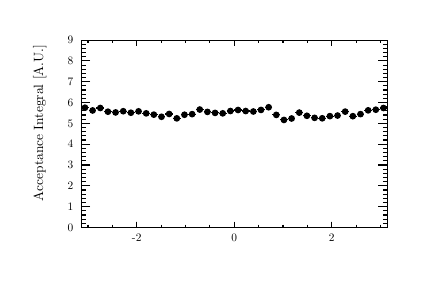
\begin{tikzpicture}
\pgfdeclareplotmark{cross} {
\pgfpathmoveto{\pgfpoint{-0.3\pgfplotmarksize}{\pgfplotmarksize}}
\pgfpathlineto{\pgfpoint{+0.3\pgfplotmarksize}{\pgfplotmarksize}}
\pgfpathlineto{\pgfpoint{+0.3\pgfplotmarksize}{0.3\pgfplotmarksize}}
\pgfpathlineto{\pgfpoint{+1\pgfplotmarksize}{0.3\pgfplotmarksize}}
\pgfpathlineto{\pgfpoint{+1\pgfplotmarksize}{-0.3\pgfplotmarksize}}
\pgfpathlineto{\pgfpoint{+0.3\pgfplotmarksize}{-0.3\pgfplotmarksize}}
\pgfpathlineto{\pgfpoint{+0.3\pgfplotmarksize}{-1.\pgfplotmarksize}}
\pgfpathlineto{\pgfpoint{-0.3\pgfplotmarksize}{-1.\pgfplotmarksize}}
\pgfpathlineto{\pgfpoint{-0.3\pgfplotmarksize}{-0.3\pgfplotmarksize}}
\pgfpathlineto{\pgfpoint{-1.\pgfplotmarksize}{-0.3\pgfplotmarksize}}
\pgfpathlineto{\pgfpoint{-1.\pgfplotmarksize}{0.3\pgfplotmarksize}}
\pgfpathlineto{\pgfpoint{-0.3\pgfplotmarksize}{0.3\pgfplotmarksize}}
\pgfpathclose
\pgfusepathqstroke
}
\pgfdeclareplotmark{cross*} {
\pgfpathmoveto{\pgfpoint{-0.3\pgfplotmarksize}{\pgfplotmarksize}}
\pgfpathlineto{\pgfpoint{+0.3\pgfplotmarksize}{\pgfplotmarksize}}
\pgfpathlineto{\pgfpoint{+0.3\pgfplotmarksize}{0.3\pgfplotmarksize}}
\pgfpathlineto{\pgfpoint{+1\pgfplotmarksize}{0.3\pgfplotmarksize}}
\pgfpathlineto{\pgfpoint{+1\pgfplotmarksize}{-0.3\pgfplotmarksize}}
\pgfpathlineto{\pgfpoint{+0.3\pgfplotmarksize}{-0.3\pgfplotmarksize}}
\pgfpathlineto{\pgfpoint{+0.3\pgfplotmarksize}{-1.\pgfplotmarksize}}
\pgfpathlineto{\pgfpoint{-0.3\pgfplotmarksize}{-1.\pgfplotmarksize}}
\pgfpathlineto{\pgfpoint{-0.3\pgfplotmarksize}{-0.3\pgfplotmarksize}}
\pgfpathlineto{\pgfpoint{-1.\pgfplotmarksize}{-0.3\pgfplotmarksize}}
\pgfpathlineto{\pgfpoint{-1.\pgfplotmarksize}{0.3\pgfplotmarksize}}
\pgfpathlineto{\pgfpoint{-0.3\pgfplotmarksize}{0.3\pgfplotmarksize}}
\pgfpathclose
\pgfusepathqfillstroke
}
\pgfdeclareplotmark{newstar} {
\pgfpathmoveto{\pgfqpoint{0pt}{\pgfplotmarksize}}
\pgfpathlineto{\pgfqpointpolar{44}{0.5\pgfplotmarksize}}
\pgfpathlineto{\pgfqpointpolar{18}{\pgfplotmarksize}}
\pgfpathlineto{\pgfqpointpolar{-20}{0.5\pgfplotmarksize}}
\pgfpathlineto{\pgfqpointpolar{-54}{\pgfplotmarksize}}
\pgfpathlineto{\pgfqpointpolar{-90}{0.5\pgfplotmarksize}}
\pgfpathlineto{\pgfqpointpolar{234}{\pgfplotmarksize}}
\pgfpathlineto{\pgfqpointpolar{198}{0.5\pgfplotmarksize}}
\pgfpathlineto{\pgfqpointpolar{162}{\pgfplotmarksize}}
\pgfpathlineto{\pgfqpointpolar{134}{0.5\pgfplotmarksize}}
\pgfpathclose
\pgfusepathqstroke
}
\pgfdeclareplotmark{newstar*} {
\pgfpathmoveto{\pgfqpoint{0pt}{\pgfplotmarksize}}
\pgfpathlineto{\pgfqpointpolar{44}{0.5\pgfplotmarksize}}
\pgfpathlineto{\pgfqpointpolar{18}{\pgfplotmarksize}}
\pgfpathlineto{\pgfqpointpolar{-20}{0.5\pgfplotmarksize}}
\pgfpathlineto{\pgfqpointpolar{-54}{\pgfplotmarksize}}
\pgfpathlineto{\pgfqpointpolar{-90}{0.5\pgfplotmarksize}}
\pgfpathlineto{\pgfqpointpolar{234}{\pgfplotmarksize}}
\pgfpathlineto{\pgfqpointpolar{198}{0.5\pgfplotmarksize}}
\pgfpathlineto{\pgfqpointpolar{162}{\pgfplotmarksize}}
\pgfpathlineto{\pgfqpointpolar{134}{0.5\pgfplotmarksize}}
\pgfpathclose
\pgfusepathqfillstroke
}
\definecolor{c}{rgb}{1,1,1};
\draw [color=c, fill=c] (0.1,0.0627517) rectangle (4.9,3.07483);
\draw [color=c, fill=c] (0.772,0.544685) rectangle (4.66,2.92423);
\definecolor{c}{rgb}{0,0,0};
\draw [c] (0.772,0.544685) -- (0.772,2.92423) -- (4.66,2.92423) -- (4.66,0.544685) -- (0.772,0.544685);
\draw [c,line width=0.4] (0.8206,2.03636) -- (0.8206,2.06591);
\draw [c,line width=0.4] (0.8206,2.06591) -- (0.8206,2.09545);
\draw [c,line width=0.4] (0.772,2.06591) -- (0.8206,2.06591);
\draw [c,line width=0.4] (0.8206,2.06591) -- (0.8692,2.06591);
\foreach \P in {(0.8206,2.06591)}{\draw[mark options={color=c,fill=c},mark size=2.402402pt,mark=*,mark size=1pt] plot coordinates {\P};}
\draw [c,line width=0.4] (0.9178,2.00134) -- (0.9178,2.03054);
\draw [c,line width=0.4] (0.9178,2.03054) -- (0.9178,2.05974);
\draw [c,line width=0.4] (0.8692,2.03054) -- (0.9178,2.03054);
\draw [c,line width=0.4] (0.9178,2.03054) -- (0.9664,2.03054);
\foreach \P in {(0.9178,2.03054)}{\draw[mark options={color=c,fill=c},mark size=2.402402pt,mark=*,mark size=1pt] plot coordinates {\P};}
\draw [c,line width=0.4] (1.015,2.03225) -- (1.015,2.06176);
\draw [c,line width=0.4] (1.015,2.06176) -- (1.015,2.09127);
\draw [c,line width=0.4] (0.9664,2.06176) -- (1.015,2.06176);
\draw [c,line width=0.4] (1.015,2.06176) -- (1.0636,2.06176);
\foreach \P in {(1.015,2.06176)}{\draw[mark options={color=c,fill=c},mark size=2.402402pt,mark=*,mark size=1pt] plot coordinates {\P};}
\draw [c,line width=0.4] (1.1122,1.98562) -- (1.1122,2.01466);
\draw [c,line width=0.4] (1.1122,2.01466) -- (1.1122,2.04371);
\draw [c,line width=0.4] (1.0636,2.01466) -- (1.1122,2.01466);
\draw [c,line width=0.4] (1.1122,2.01466) -- (1.1608,2.01466);
\foreach \P in {(1.1122,2.01466)}{\draw[mark options={color=c,fill=c},mark size=2.402402pt,mark=*,mark size=1pt] plot coordinates {\P};}
\draw [c,line width=0.4] (1.2094,1.97657) -- (1.2094,2.00552);
\draw [c,line width=0.4] (1.2094,2.00552) -- (1.2094,2.03448);
\draw [c,line width=0.4] (1.1608,2.00552) -- (1.2094,2.00552);
\draw [c,line width=0.4] (1.2094,2.00552) -- (1.258,2.00552);
\foreach \P in {(1.2094,2.00552)}{\draw[mark options={color=c,fill=c},mark size=2.402402pt,mark=*,mark size=1pt] plot coordinates {\P};}
\draw [c,line width=0.4] (1.3066,1.99186) -- (1.3066,2.02097);
\draw [c,line width=0.4] (1.3066,2.02097) -- (1.3066,2.05008);
\draw [c,line width=0.4] (1.258,2.02097) -- (1.3066,2.02097);
\draw [c,line width=0.4] (1.3066,2.02097) -- (1.3552,2.02097);
\foreach \P in {(1.3066,2.02097)}{\draw[mark options={color=c,fill=c},mark size=2.402402pt,mark=*,mark size=1pt] plot coordinates {\P};}
\draw [c,line width=0.4] (1.4038,1.97265) -- (1.4038,2.00156);
\draw [c,line width=0.4] (1.4038,2.00156) -- (1.4038,2.03048);
\draw [c,line width=0.4] (1.3552,2.00156) -- (1.4038,2.00156);
\draw [c,line width=0.4] (1.4038,2.00156) -- (1.4524,2.00156);
\foreach \P in {(1.4038,2.00156)}{\draw[mark options={color=c,fill=c},mark size=2.402402pt,mark=*,mark size=1pt] plot coordinates {\P};}
\draw [c,line width=0.4] (1.501,1.99018) -- (1.501,2.01927);
\draw [c,line width=0.4] (1.501,2.01927) -- (1.501,2.04836);
\draw [c,line width=0.4] (1.4524,2.01927) -- (1.501,2.01927);
\draw [c,line width=0.4] (1.501,2.01927) -- (1.5496,2.01927);
\foreach \P in {(1.501,2.01927)}{\draw[mark options={color=c,fill=c},mark size=2.402402pt,mark=*,mark size=1pt] plot coordinates {\P};}
\draw [c,line width=0.4] (1.5982,1.96487) -- (1.5982,1.99371);
\draw [c,line width=0.4] (1.5982,1.99371) -- (1.5982,2.02254);
\draw [c,line width=0.4] (1.5496,1.99371) -- (1.5982,1.99371);
\draw [c,line width=0.4] (1.5982,1.99371) -- (1.6468,1.99371);
\foreach \P in {(1.5982,1.99371)}{\draw[mark options={color=c,fill=c},mark size=2.402402pt,mark=*,mark size=1pt] plot coordinates {\P};}
\draw [c,line width=0.4] (1.6954,1.94869) -- (1.6954,1.97737);
\draw [c,line width=0.4] (1.6954,1.97737) -- (1.6954,2.00604);
\draw [c,line width=0.4] (1.6468,1.97737) -- (1.6954,1.97737);
\draw [c,line width=0.4] (1.6954,1.97737) -- (1.744,1.97737);
\foreach \P in {(1.6954,1.97737)}{\draw[mark options={color=c,fill=c},mark size=2.402402pt,mark=*,mark size=1pt] plot coordinates {\P};}
\draw [c,line width=0.4] (1.7926,1.92168) -- (1.7926,1.95008);
\draw [c,line width=0.4] (1.7926,1.95008) -- (1.7926,1.97848);
\draw [c,line width=0.4] (1.744,1.95008) -- (1.7926,1.95008);
\draw [c,line width=0.4] (1.7926,1.95008) -- (1.8412,1.95008);
\foreach \P in {(1.7926,1.95008)}{\draw[mark options={color=c,fill=c},mark size=2.402402pt,mark=*,mark size=1pt] plot coordinates {\P};}
\draw [c,line width=0.4] (1.8898,1.95726) -- (1.8898,1.98602);
\draw [c,line width=0.4] (1.8898,1.98602) -- (1.8898,2.01478);
\draw [c,line width=0.4] (1.8412,1.98602) -- (1.8898,1.98602);
\draw [c,line width=0.4] (1.8898,1.98602) -- (1.9384,1.98602);
\foreach \P in {(1.8898,1.98602)}{\draw[mark options={color=c,fill=c},mark size=2.402402pt,mark=*,mark size=1pt] plot coordinates {\P};}
\draw [c,line width=0.4] (1.987,1.90193) -- (1.987,1.93013);
\draw [c,line width=0.4] (1.987,1.93013) -- (1.987,1.95832);
\draw [c,line width=0.4] (1.9384,1.93013) -- (1.987,1.93013);
\draw [c,line width=0.4] (1.987,1.93013) -- (2.0356,1.93013);
\foreach \P in {(1.987,1.93013)}{\draw[mark options={color=c,fill=c},mark size=2.402402pt,mark=*,mark size=1pt] plot coordinates {\P};}
\draw [c,line width=0.4] (2.0842,1.94739) -- (2.0842,1.97605);
\draw [c,line width=0.4] (2.0842,1.97605) -- (2.0842,2.00471);
\draw [c,line width=0.4] (2.0356,1.97605) -- (2.0842,1.97605);
\draw [c,line width=0.4] (2.0842,1.97605) -- (2.1328,1.97605);
\foreach \P in {(2.0842,1.97605)}{\draw[mark options={color=c,fill=c},mark size=2.402402pt,mark=*,mark size=1pt] plot coordinates {\P};}
\draw [c,line width=0.4] (2.1814,1.95498) -- (2.1814,1.98371);
\draw [c,line width=0.4] (2.1814,1.98371) -- (2.1814,2.01245);
\draw [c,line width=0.4] (2.1328,1.98371) -- (2.1814,1.98371);
\draw [c,line width=0.4] (2.1814,1.98371) -- (2.23,1.98371);
\foreach \P in {(2.1814,1.98371)}{\draw[mark options={color=c,fill=c},mark size=2.402402pt,mark=*,mark size=1pt] plot coordinates {\P};}
\draw [c,line width=0.4] (2.2786,2.01279) -- (2.2786,2.0421);
\draw [c,line width=0.4] (2.2786,2.0421) -- (2.2786,2.07142);
\draw [c,line width=0.4] (2.23,2.0421) -- (2.2786,2.0421);
\draw [c,line width=0.4] (2.2786,2.0421) -- (2.3272,2.0421);
\foreach \P in {(2.2786,2.0421)}{\draw[mark options={color=c,fill=c},mark size=2.402402pt,mark=*,mark size=1pt] plot coordinates {\P};}
\draw [c,line width=0.4] (2.3758,1.98336) -- (2.3758,2.01238);
\draw [c,line width=0.4] (2.3758,2.01238) -- (2.3758,2.0414);
\draw [c,line width=0.4] (2.3272,2.01238) -- (2.3758,2.01238);
\draw [c,line width=0.4] (2.3758,2.01238) -- (2.4244,2.01238);
\foreach \P in {(2.3758,2.01238)}{\draw[mark options={color=c,fill=c},mark size=2.402402pt,mark=*,mark size=1pt] plot coordinates {\P};}
\draw [c,line width=0.4] (2.473,1.97066) -- (2.473,1.99956);
\draw [c,line width=0.4] (2.473,1.99956) -- (2.473,2.02845);
\draw [c,line width=0.4] (2.4244,1.99956) -- (2.473,1.99956);
\draw [c,line width=0.4] (2.473,1.99956) -- (2.5216,1.99956);
\foreach \P in {(2.473,1.99956)}{\draw[mark options={color=c,fill=c},mark size=2.402402pt,mark=*,mark size=1pt] plot coordinates {\P};}
\draw [c,line width=0.4] (2.5702,1.96511) -- (2.5702,1.99395);
\draw [c,line width=0.4] (2.5702,1.99395) -- (2.5702,2.02279);
\draw [c,line width=0.4] (2.5216,1.99395) -- (2.5702,1.99395);
\draw [c,line width=0.4] (2.5702,1.99395) -- (2.6188,1.99395);
\foreach \P in {(2.5702,1.99395)}{\draw[mark options={color=c,fill=c},mark size=2.402402pt,mark=*,mark size=1pt] plot coordinates {\P};}
\draw [c,line width=0.4] (2.6674,1.99431) -- (2.6674,2.02344);
\draw [c,line width=0.4] (2.6674,2.02344) -- (2.6674,2.05258);
\draw [c,line width=0.4] (2.6188,2.02344) -- (2.6674,2.02344);
\draw [c,line width=0.4] (2.6674,2.02344) -- (2.716,2.02344);
\foreach \P in {(2.6674,2.02344)}{\draw[mark options={color=c,fill=c},mark size=2.402402pt,mark=*,mark size=1pt] plot coordinates {\P};}
\draw [c,line width=0.4] (2.7646,2.00703) -- (2.7646,2.03629);
\draw [c,line width=0.4] (2.7646,2.03629) -- (2.7646,2.06554);
\draw [c,line width=0.4] (2.716,2.03629) -- (2.7646,2.03629);
\draw [c,line width=0.4] (2.7646,2.03629) -- (2.8132,2.03629);
\foreach \P in {(2.7646,2.03629)}{\draw[mark options={color=c,fill=c},mark size=2.402402pt,mark=*,mark size=1pt] plot coordinates {\P};}
\draw [c,line width=0.4] (2.8618,1.99411) -- (2.8618,2.02324);
\draw [c,line width=0.4] (2.8618,2.02324) -- (2.8618,2.05237);
\draw [c,line width=0.4] (2.8132,2.02324) -- (2.8618,2.02324);
\draw [c,line width=0.4] (2.8618,2.02324) -- (2.9104,2.02324);
\foreach \P in {(2.8618,2.02324)}{\draw[mark options={color=c,fill=c},mark size=2.402402pt,mark=*,mark size=1pt] plot coordinates {\P};}
\draw [c,line width=0.4] (2.959,1.98815) -- (2.959,2.01722);
\draw [c,line width=0.4] (2.959,2.01722) -- (2.959,2.04629);
\draw [c,line width=0.4] (2.9104,2.01722) -- (2.959,2.01722);
\draw [c,line width=0.4] (2.959,2.01722) -- (3.0076,2.01722);
\foreach \P in {(2.959,2.01722)}{\draw[mark options={color=c,fill=c},mark size=2.402402pt,mark=*,mark size=1pt] plot coordinates {\P};}
\draw [c,line width=0.4] (3.0562,2.0079) -- (3.0562,2.03716);
\draw [c,line width=0.4] (3.0562,2.03716) -- (3.0562,2.06643);
\draw [c,line width=0.4] (3.0076,2.03716) -- (3.0562,2.03716);
\draw [c,line width=0.4] (3.0562,2.03716) -- (3.1048,2.03716);
\foreach \P in {(3.0562,2.03716)}{\draw[mark options={color=c,fill=c},mark size=2.402402pt,mark=*,mark size=1pt] plot coordinates {\P};}
\draw [c,line width=0.4] (3.1534,2.04165) -- (3.1534,2.07125);
\draw [c,line width=0.4] (3.1534,2.07125) -- (3.1534,2.10085);
\draw [c,line width=0.4] (3.1048,2.07125) -- (3.1534,2.07125);
\draw [c,line width=0.4] (3.1534,2.07125) -- (3.202,2.07125);
\foreach \P in {(3.1534,2.07125)}{\draw[mark options={color=c,fill=c},mark size=2.402402pt,mark=*,mark size=1pt] plot coordinates {\P};}
\draw [c,line width=0.4] (3.2506,1.94565) -- (3.2506,1.97429);
\draw [c,line width=0.4] (3.2506,1.97429) -- (3.2506,2.00294);
\draw [c,line width=0.4] (3.202,1.97429) -- (3.2506,1.97429);
\draw [c,line width=0.4] (3.2506,1.97429) -- (3.2992,1.97429);
\foreach \P in {(3.2506,1.97429)}{\draw[mark options={color=c,fill=c},mark size=2.402402pt,mark=*,mark size=1pt] plot coordinates {\P};}
\draw [c,line width=0.4] (3.3478,1.88222) -- (3.3478,1.91022);
\draw [c,line width=0.4] (3.3478,1.91022) -- (3.3478,1.93821);
\draw [c,line width=0.4] (3.2992,1.91022) -- (3.3478,1.91022);
\draw [c,line width=0.4] (3.3478,1.91022) -- (3.3964,1.91022);
\foreach \P in {(3.3478,1.91022)}{\draw[mark options={color=c,fill=c},mark size=2.402402pt,mark=*,mark size=1pt] plot coordinates {\P};}
\draw [c,line width=0.4] (3.445,1.90023) -- (3.445,1.92841);
\draw [c,line width=0.4] (3.445,1.92841) -- (3.445,1.95659);
\draw [c,line width=0.4] (3.3964,1.92841) -- (3.445,1.92841);
\draw [c,line width=0.4] (3.445,1.92841) -- (3.4936,1.92841);
\foreach \P in {(3.445,1.92841)}{\draw[mark options={color=c,fill=c},mark size=2.402402pt,mark=*,mark size=1pt] plot coordinates {\P};}
\draw [c,line width=0.4] (3.5422,1.97428) -- (3.5422,2.00321);
\draw [c,line width=0.4] (3.5422,2.00321) -- (3.5422,2.03214);
\draw [c,line width=0.4] (3.4936,2.00321) -- (3.5422,2.00321);
\draw [c,line width=0.4] (3.5422,2.00321) -- (3.5908,2.00321);
\foreach \P in {(3.5422,2.00321)}{\draw[mark options={color=c,fill=c},mark size=2.402402pt,mark=*,mark size=1pt] plot coordinates {\P};}
\draw [c,line width=0.4] (3.6394,1.93423) -- (3.6394,1.96275);
\draw [c,line width=0.4] (3.6394,1.96275) -- (3.6394,1.99128);
\draw [c,line width=0.4] (3.5908,1.96275) -- (3.6394,1.96275);
\draw [c,line width=0.4] (3.6394,1.96275) -- (3.688,1.96275);
\foreach \P in {(3.6394,1.96275)}{\draw[mark options={color=c,fill=c},mark size=2.402402pt,mark=*,mark size=1pt] plot coordinates {\P};}
\draw [c,line width=0.4] (3.7366,1.90843) -- (3.7366,1.93669);
\draw [c,line width=0.4] (3.7366,1.93669) -- (3.7366,1.96496);
\draw [c,line width=0.4] (3.688,1.93669) -- (3.7366,1.93669);
\draw [c,line width=0.4] (3.7366,1.93669) -- (3.7852,1.93669);
\foreach \P in {(3.7366,1.93669)}{\draw[mark options={color=c,fill=c},mark size=2.402402pt,mark=*,mark size=1pt] plot coordinates {\P};}
\draw [c,line width=0.4] (3.8338,1.90278) -- (3.8338,1.93099);
\draw [c,line width=0.4] (3.8338,1.93099) -- (3.8338,1.9592);
\draw [c,line width=0.4] (3.7852,1.93099) -- (3.8338,1.93099);
\draw [c,line width=0.4] (3.8338,1.93099) -- (3.8824,1.93099);
\foreach \P in {(3.8338,1.93099)}{\draw[mark options={color=c,fill=c},mark size=2.402402pt,mark=*,mark size=1pt] plot coordinates {\P};}
\draw [c,line width=0.4] (3.931,1.9298) -- (3.931,1.95828);
\draw [c,line width=0.4] (3.931,1.95828) -- (3.931,1.98676);
\draw [c,line width=0.4] (3.8824,1.95828) -- (3.931,1.95828);
\draw [c,line width=0.4] (3.931,1.95828) -- (3.9796,1.95828);
\foreach \P in {(3.931,1.95828)}{\draw[mark options={color=c,fill=c},mark size=2.402402pt,mark=*,mark size=1pt] plot coordinates {\P};}
\draw [c,line width=0.4] (4.0282,1.9373) -- (4.0282,1.96586);
\draw [c,line width=0.4] (4.0282,1.96586) -- (4.0282,1.99441);
\draw [c,line width=0.4] (3.9796,1.96586) -- (4.0282,1.96586);
\draw [c,line width=0.4] (4.0282,1.96586) -- (4.0768,1.96586);
\foreach \P in {(4.0282,1.96586)}{\draw[mark options={color=c,fill=c},mark size=2.402402pt,mark=*,mark size=1pt] plot coordinates {\P};}
\draw [c,line width=0.4] (4.1254,1.98665) -- (4.1254,2.0157);
\draw [c,line width=0.4] (4.1254,2.0157) -- (4.1254,2.04476);
\draw [c,line width=0.4] (4.0768,2.0157) -- (4.1254,2.0157);
\draw [c,line width=0.4] (4.1254,2.0157) -- (4.174,2.0157);
\foreach \P in {(4.1254,2.0157)}{\draw[mark options={color=c,fill=c},mark size=2.402402pt,mark=*,mark size=1pt] plot coordinates {\P};}
\draw [c,line width=0.4] (4.2226,1.92943) -- (4.2226,1.95791);
\draw [c,line width=0.4] (4.2226,1.95791) -- (4.2226,1.98638);
\draw [c,line width=0.4] (4.174,1.95791) -- (4.2226,1.95791);
\draw [c,line width=0.4] (4.2226,1.95791) -- (4.2712,1.95791);
\foreach \P in {(4.2226,1.95791)}{\draw[mark options={color=c,fill=c},mark size=2.402402pt,mark=*,mark size=1pt] plot coordinates {\P};}
\draw [c,line width=0.4] (4.3198,1.95516) -- (4.3198,1.9839);
\draw [c,line width=0.4] (4.3198,1.9839) -- (4.3198,2.01264);
\draw [c,line width=0.4] (4.2712,1.9839) -- (4.3198,1.9839);
\draw [c,line width=0.4] (4.3198,1.9839) -- (4.3684,1.9839);
\foreach \P in {(4.3198,1.9839)}{\draw[mark options={color=c,fill=c},mark size=2.402402pt,mark=*,mark size=1pt] plot coordinates {\P};}
\draw [c,line width=0.4] (4.417,2.00274) -- (4.417,2.03195);
\draw [c,line width=0.4] (4.417,2.03195) -- (4.417,2.06117);
\draw [c,line width=0.4] (4.3684,2.03195) -- (4.417,2.03195);
\draw [c,line width=0.4] (4.417,2.03195) -- (4.4656,2.03195);
\foreach \P in {(4.417,2.03195)}{\draw[mark options={color=c,fill=c},mark size=2.402402pt,mark=*,mark size=1pt] plot coordinates {\P};}
\draw [c,line width=0.4] (4.5142,2.01071) -- (4.5142,2.04);
\draw [c,line width=0.4] (4.5142,2.04) -- (4.5142,2.0693);
\draw [c,line width=0.4] (4.4656,2.04) -- (4.5142,2.04);
\draw [c,line width=0.4] (4.5142,2.04) -- (4.5628,2.04);
\foreach \P in {(4.5142,2.04)}{\draw[mark options={color=c,fill=c},mark size=2.402402pt,mark=*,mark size=1pt] plot coordinates {\P};}
\draw [c,line width=0.4] (4.6114,2.03217) -- (4.6114,2.06168);
\draw [c,line width=0.4] (4.6114,2.06168) -- (4.6114,2.09118);
\draw [c,line width=0.4] (4.5628,2.06168) -- (4.6114,2.06168);
\draw [c,line width=0.4] (4.6114,2.06168) -- (4.66,2.06168);
\foreach \P in {(4.6114,2.06168)}{\draw[mark options={color=c,fill=c},mark size=2.402402pt,mark=*,mark size=1pt] plot coordinates {\P};}
\draw [c,line width=0.4] (0.772,0.544685) -- (4.66,0.544685);
\draw [anchor= east] (4.66,0.215042) node[scale=0.485847, rotate=0]{$\phihel$};
\draw [c,line width=0.4] (1.47778,0.617878) -- (1.47778,0.544685);
\draw [c,line width=0.4] (1.78734,0.581281) -- (1.78734,0.544685);
\draw [c,line width=0.4] (2.09689,0.581281) -- (2.09689,0.544685);
\draw [c,line width=0.4] (2.40645,0.581281) -- (2.40645,0.544685);
\draw [c,line width=0.4] (2.716,0.617878) -- (2.716,0.544685);
\draw [c,line width=0.4] (3.02555,0.581281) -- (3.02555,0.544685);
\draw [c,line width=0.4] (3.33511,0.581281) -- (3.33511,0.544685);
\draw [c,line width=0.4] (3.64466,0.581281) -- (3.64466,0.544685);
\draw [c,line width=0.4] (3.95422,0.617878) -- (3.95422,0.544685);
\draw [c,line width=0.4] (1.47778,0.617878) -- (1.47778,0.544685);
\draw [c,line width=0.4] (1.16823,0.581281) -- (1.16823,0.544685);
\draw [c,line width=0.4] (0.858675,0.581281) -- (0.858675,0.544685);
\draw [c,line width=0.4] (3.95422,0.617878) -- (3.95422,0.544685);
\draw [c,line width=0.4] (4.26377,0.581281) -- (4.26377,0.544685);
\draw [c,line width=0.4] (4.57332,0.581281) -- (4.57332,0.544685);
\draw [anchor=base] (1.47778,0.369984) node[scale=0.411101, rotate=0]{-2};
\draw [anchor=base] (2.716,0.369984) node[scale=0.411101, rotate=0]{0};
\draw [anchor=base] (3.95422,0.369984) node[scale=0.411101, rotate=0]{2};
\draw [c,line width=0.4] (0.772,2.92423) -- (4.66,2.92423);
\draw [c,line width=0.4] (1.47778,2.85103) -- (1.47778,2.92423);
\draw [c,line width=0.4] (1.78734,2.88763) -- (1.78734,2.92423);
\draw [c,line width=0.4] (2.09689,2.88763) -- (2.09689,2.92423);
\draw [c,line width=0.4] (2.40645,2.88763) -- (2.40645,2.92423);
\draw [c,line width=0.4] (2.716,2.85103) -- (2.716,2.92423);
\draw [c,line width=0.4] (3.02555,2.88763) -- (3.02555,2.92423);
\draw [c,line width=0.4] (3.33511,2.88763) -- (3.33511,2.92423);
\draw [c,line width=0.4] (3.64466,2.88763) -- (3.64466,2.92423);
\draw [c,line width=0.4] (3.95422,2.85103) -- (3.95422,2.92423);
\draw [c,line width=0.4] (1.47778,2.85103) -- (1.47778,2.92423);
\draw [c,line width=0.4] (1.16823,2.88763) -- (1.16823,2.92423);
\draw [c,line width=0.4] (0.858675,2.88763) -- (0.858675,2.92423);
\draw [c,line width=0.4] (3.95422,2.85103) -- (3.95422,2.92423);
\draw [c,line width=0.4] (4.26377,2.88763) -- (4.26377,2.92423);
\draw [c,line width=0.4] (4.57332,2.88763) -- (4.57332,2.92423);
\draw [c,line width=0.4] (0.772,0.544685) -- (0.772,2.92423);
\draw [anchor= east] (0.246688,2.92423) node[scale=0.485847, rotate=90]{Acceptance Integral [A.U.]};
\draw [c,line width=0.4] (0.88576,0.544685) -- (0.772,0.544685);
\draw [c,line width=0.4] (0.82888,0.597563) -- (0.772,0.597563);
\draw [c,line width=0.4] (0.82888,0.650442) -- (0.772,0.650442);
\draw [c,line width=0.4] (0.82888,0.703321) -- (0.772,0.703321);
\draw [c,line width=0.4] (0.82888,0.7562) -- (0.772,0.7562);
\draw [c,line width=0.4] (0.88576,0.809078) -- (0.772,0.809078);
\draw [c,line width=0.4] (0.82888,0.861957) -- (0.772,0.861957);
\draw [c,line width=0.4] (0.82888,0.914836) -- (0.772,0.914836);
\draw [c,line width=0.4] (0.82888,0.967715) -- (0.772,0.967715);
\draw [c,line width=0.4] (0.82888,1.02059) -- (0.772,1.02059);
\draw [c,line width=0.4] (0.88576,1.07347) -- (0.772,1.07347);
\draw [c,line width=0.4] (0.82888,1.12635) -- (0.772,1.12635);
\draw [c,line width=0.4] (0.82888,1.17923) -- (0.772,1.17923);
\draw [c,line width=0.4] (0.82888,1.23211) -- (0.772,1.23211);
\draw [c,line width=0.4] (0.82888,1.28499) -- (0.772,1.28499);
\draw [c,line width=0.4] (0.88576,1.33787) -- (0.772,1.33787);
\draw [c,line width=0.4] (0.82888,1.39074) -- (0.772,1.39074);
\draw [c,line width=0.4] (0.82888,1.44362) -- (0.772,1.44362);
\draw [c,line width=0.4] (0.82888,1.4965) -- (0.772,1.4965);
\draw [c,line width=0.4] (0.82888,1.54938) -- (0.772,1.54938);
\draw [c,line width=0.4] (0.88576,1.60226) -- (0.772,1.60226);
\draw [c,line width=0.4] (0.82888,1.65514) -- (0.772,1.65514);
\draw [c,line width=0.4] (0.82888,1.70802) -- (0.772,1.70802);
\draw [c,line width=0.4] (0.82888,1.7609) -- (0.772,1.7609);
\draw [c,line width=0.4] (0.82888,1.81377) -- (0.772,1.81377);
\draw [c,line width=0.4] (0.88576,1.86665) -- (0.772,1.86665);
\draw [c,line width=0.4] (0.82888,1.91953) -- (0.772,1.91953);
\draw [c,line width=0.4] (0.82888,1.97241) -- (0.772,1.97241);
\draw [c,line width=0.4] (0.82888,2.02529) -- (0.772,2.02529);
\draw [c,line width=0.4] (0.82888,2.07817) -- (0.772,2.07817);
\draw [c,line width=0.4] (0.88576,2.13105) -- (0.772,2.13105);
\draw [c,line width=0.4] (0.82888,2.18393) -- (0.772,2.18393);
\draw [c,line width=0.4] (0.82888,2.2368) -- (0.772,2.2368);
\draw [c,line width=0.4] (0.82888,2.28968) -- (0.772,2.28968);
\draw [c,line width=0.4] (0.82888,2.34256) -- (0.772,2.34256);
\draw [c,line width=0.4] (0.88576,2.39544) -- (0.772,2.39544);
\draw [c,line width=0.4] (0.82888,2.44832) -- (0.772,2.44832);
\draw [c,line width=0.4] (0.82888,2.5012) -- (0.772,2.5012);
\draw [c,line width=0.4] (0.82888,2.55408) -- (0.772,2.55408);
\draw [c,line width=0.4] (0.82888,2.60696) -- (0.772,2.60696);
\draw [c,line width=0.4] (0.88576,2.65983) -- (0.772,2.65983);
\draw [c,line width=0.4] (0.82888,2.71271) -- (0.772,2.71271);
\draw [c,line width=0.4] (0.82888,2.76559) -- (0.772,2.76559);
\draw [c,line width=0.4] (0.82888,2.81847) -- (0.772,2.81847);
\draw [c,line width=0.4] (0.82888,2.87135) -- (0.772,2.87135);
\draw [c,line width=0.4] (0.88576,2.92423) -- (0.772,2.92423);
\draw [anchor= east] (0.724,0.544685) node[scale=0.411101, rotate=0]{0};
\draw [anchor= east] (0.724,0.809078) node[scale=0.411101, rotate=0]{1};
\draw [anchor= east] (0.724,1.07347) node[scale=0.411101, rotate=0]{2};
\draw [anchor= east] (0.724,1.33787) node[scale=0.411101, rotate=0]{3};
\draw [anchor= east] (0.724,1.60226) node[scale=0.411101, rotate=0]{4};
\draw [anchor= east] (0.724,1.86665) node[scale=0.411101, rotate=0]{5};
\draw [anchor= east] (0.724,2.13105) node[scale=0.411101, rotate=0]{6};
\draw [anchor= east] (0.724,2.39544) node[scale=0.411101, rotate=0]{7};
\draw [anchor= east] (0.724,2.65983) node[scale=0.411101, rotate=0]{8};
\draw [anchor= east] (0.724,2.92423) node[scale=0.411101, rotate=0]{9};
\draw [c,line width=0.4] (4.66,0.544685) -- (4.66,2.92423);
\draw [c,line width=0.4] (4.54624,0.544685) -- (4.66,0.544685);
\draw [c,line width=0.4] (4.60312,0.597563) -- (4.66,0.597563);
\draw [c,line width=0.4] (4.60312,0.650442) -- (4.66,0.650442);
\draw [c,line width=0.4] (4.60312,0.703321) -- (4.66,0.703321);
\draw [c,line width=0.4] (4.60312,0.7562) -- (4.66,0.7562);
\draw [c,line width=0.4] (4.54624,0.809078) -- (4.66,0.809078);
\draw [c,line width=0.4] (4.60312,0.861957) -- (4.66,0.861957);
\draw [c,line width=0.4] (4.60312,0.914836) -- (4.66,0.914836);
\draw [c,line width=0.4] (4.60312,0.967715) -- (4.66,0.967715);
\draw [c,line width=0.4] (4.60312,1.02059) -- (4.66,1.02059);
\draw [c,line width=0.4] (4.54624,1.07347) -- (4.66,1.07347);
\draw [c,line width=0.4] (4.60312,1.12635) -- (4.66,1.12635);
\draw [c,line width=0.4] (4.60312,1.17923) -- (4.66,1.17923);
\draw [c,line width=0.4] (4.60312,1.23211) -- (4.66,1.23211);
\draw [c,line width=0.4] (4.60312,1.28499) -- (4.66,1.28499);
\draw [c,line width=0.4] (4.54624,1.33787) -- (4.66,1.33787);
\draw [c,line width=0.4] (4.60312,1.39074) -- (4.66,1.39074);
\draw [c,line width=0.4] (4.60312,1.44362) -- (4.66,1.44362);
\draw [c,line width=0.4] (4.60312,1.4965) -- (4.66,1.4965);
\draw [c,line width=0.4] (4.60312,1.54938) -- (4.66,1.54938);
\draw [c,line width=0.4] (4.54624,1.60226) -- (4.66,1.60226);
\draw [c,line width=0.4] (4.60312,1.65514) -- (4.66,1.65514);
\draw [c,line width=0.4] (4.60312,1.70802) -- (4.66,1.70802);
\draw [c,line width=0.4] (4.60312,1.7609) -- (4.66,1.7609);
\draw [c,line width=0.4] (4.60312,1.81377) -- (4.66,1.81377);
\draw [c,line width=0.4] (4.54624,1.86665) -- (4.66,1.86665);
\draw [c,line width=0.4] (4.60312,1.91953) -- (4.66,1.91953);
\draw [c,line width=0.4] (4.60312,1.97241) -- (4.66,1.97241);
\draw [c,line width=0.4] (4.60312,2.02529) -- (4.66,2.02529);
\draw [c,line width=0.4] (4.60312,2.07817) -- (4.66,2.07817);
\draw [c,line width=0.4] (4.54624,2.13105) -- (4.66,2.13105);
\draw [c,line width=0.4] (4.60312,2.18393) -- (4.66,2.18393);
\draw [c,line width=0.4] (4.60312,2.2368) -- (4.66,2.2368);
\draw [c,line width=0.4] (4.60312,2.28968) -- (4.66,2.28968);
\draw [c,line width=0.4] (4.60312,2.34256) -- (4.66,2.34256);
\draw [c,line width=0.4] (4.54624,2.39544) -- (4.66,2.39544);
\draw [c,line width=0.4] (4.60312,2.44832) -- (4.66,2.44832);
\draw [c,line width=0.4] (4.60312,2.5012) -- (4.66,2.5012);
\draw [c,line width=0.4] (4.60312,2.55408) -- (4.66,2.55408);
\draw [c,line width=0.4] (4.60312,2.60696) -- (4.66,2.60696);
\draw [c,line width=0.4] (4.54624,2.65983) -- (4.66,2.65983);
\draw [c,line width=0.4] (4.60312,2.71271) -- (4.66,2.71271);
\draw [c,line width=0.4] (4.60312,2.76559) -- (4.66,2.76559);
\draw [c,line width=0.4] (4.60312,2.81847) -- (4.66,2.81847);
\draw [c,line width=0.4] (4.60312,2.87135) -- (4.66,2.87135);
\draw [c,line width=0.4] (4.54624,2.92423) -- (4.66,2.92423);
\end{tikzpicture}
}
    \caption{}
    \label{angAcc_phi}
  \end{subfigure}
  \caption{Angular acceptance shape from simulated data. Each event in the simulated sample has been weighted with the inverse integral 
           of the \pdf that was used to generate them with, resulting to those three distributions that give a feeling of the acceptance shape.
           The scale of the $y$-axis is arbitrary.}
\end{figure}

\subsubsection{Acceptance parametrization}
\label{Acceptance parametrization}
As for the parametrization of the angular acceptance there are at least two ways to proceed,
namely the \emph{efficiency moments} \cite{jeroenThesis} and the \emph{normalization weights} \cite{tristanThesis,jeroenThesis}. 
The current analysis implements the first one, where the efficiency function is parametrized using orthogonal functions (nicely
combined with the angular description formalism in the previous subsection). Such a parameterization can be seen in the next equation 
\equref{eff_func}. The symbol $\effbase$ is introduced as a shorter notation.

\begin{center}
\begin{equation}
  \epsilon(\Omega) = \sum_{ijk} \; \moment{i}{j}{k} \; P_i^0(\cos\thetaK) \; Y_{jk}(\cos\thetamu,\phihel) \equiv \moment{i}{j}{k} \; \effbase
  \label{eff_func}
\end{equation}
\end{center}

\noindent where the familiar from the previous section spherical harmonics ($Y$) and associated Legendre polynomials ($P$) show up as the basis
functions on which the angular acceptance is decomposed to the $PY$ basis by means of the coefficients $c^i_{k}$, hereafter efficiency moments (or simply moments). 
The reason of choosing the particular parameterizations is obviously for the known analytical integrals of product of two $P$ or $Y$. 
Following the above parameterizations one just needs to choose a set of $c^i_{jk}$ and find a way compute them. In principle there are infinite efficiency moments
since the sum in \equref{eff_func} runs through all possible values of the $ijk$ indices. However in practice only a small number of efficiency moments 
contribute significantly to the proper description of the angular acceptance shape. The efficiency moments used to describe the acceptance 
shape are shown in the first column of \tabref{eff_moms_table}. The choice of those particular moments is connected to an important issue with the acceptance 
structure close to $\cos\thetaK=1$ and it is addressed at the end of the current section.   

In order for the efficiency moments $c^i_{jk}$ to be computed a definition of the efficiency is necessary. Note that this computation relies on 
simulated data where all the generating conditions are known. The efficiency then is defined as the ratio of two angular dependent \pdfs, namely
\Pobs and \Pgen. The first is the angular \pdf that the simulated data follow after all stages of selection, whereas
the later is the angular \pdf which the simulated data have been generated with. It follows that the efficiency is defined as the ratio of the first
over the later and it is shown in equation \equref{eff_def}.

\begin{center}
\begin{equation}
  \epsilon(\Omega) \equiv \frac{\Pobs}{\Pgen}
  \label{eff_def}
\end{equation}
\end{center}

\noindent Computing the efficiency moments is done by projecting the efficiency as defined in \equref{eff_def} on the orthogonal $PY$ basis.
This projection is shown in \equref{eff_moms_def}. Where the factor $j+\frac{1}{2}$ is used to account for the fact that the associated Legendre 
polynomials form an orthogonal basis but in fact the orthonormal behavior is required to properly compute the efficiency moments. 


\begin{center}
\begin{align}
   c^i_{jk}  \equiv &(j + \frac{1}{2}) \; \int \; d\Omega \; \effbase \; \epsilon(\Omega) \nonumber \\ 
                 = &(j + \frac{1}{2}) \; \int \; d\Omega \; \Pobs \; \frac{\effbase}{\Pgen}  
  \label{eff_moms_def}
\end{align}
\end{center}

\noindent The last step in the calculation of the efficiency moments is the computation of the integral in \equref{eff_moms_def}.
This is done by means of simulated data and the integral is computed following the concept of Monte Carlo integration. This implies
that the integral in \equref{eff_moms_def} can be estimated by a sum over the simulated data (which they have passed through the exact
same steps selection as the real data) as shown in \equref{eff_moms_calc}.   

\begin{center}
\begin{equation}
  E\left[ \int \; d\Omega \; \effbase \frac{\Pobs}{\Pgen} \right] = \frac{1}{\Nobs} \sum_e^{\Nobs} \frac{\effbase}{\Pgen}  
  \label{eff_moms_calc}
\end{equation}
\end{center}

\noindent Combining \equref{eff_moms_def} and \equref{eff_moms_calc} the final expression for computing the efficiency moments is shown
in \equref{eff_moms_calc_final} and the result of the computations can be found it table \tabref{eff_moms_table}/  

\begin{center}
\begin{equation}
 c^i_{jk} \equiv (j + \frac{1}{2})  \frac{1}{\Nobs} \sum_e^{\Nobs} \frac{\effbase}{\Pgen}  
  \label{eff_moms_calc_final}
\end{equation}
\end{center}

\begin{table}[h]
  \centering 
  \renewcommand{\arraystretch}{1.2}
  \begin{tabular}{ccc}
    \hline
    moment & central value & standard deviation \\
    \hline
  $\moment{0}{0}{0}$   & \text{constrained}  &  -  \\
  $\moment{1}{0}{0}$   & -2.0982  &  0.0084  \\
  $\moment{2}{0}{0}$   & -1.9116  &  0.0126  \\
  $\moment{3}{0}{0}$   & -0.0317  &  0.0151  \\
  $\moment{4}{0}{0}$   & +0.1146  &  0.0175  \\
  $\moment{5}{0}{0}$   & +0.1384  &  0.0193  \\
  $\moment{0}{2}{0}$   & +0.2820  &  0.0066  \\
  $\moment{0}{2}{2}$   & +0.0612  &  0.0058  \\
  $\moment{0}{4}{0}$   & +0.0864  &  0.0066  \\
  $\moment{1}{2}{0}$   & -0.1900  &  0.0115  \\
  $\moment{1}{4}{0}$   & -0.0720  &  0.0118  \\
  $\moment{2}{2}{0}$   & -0.1315  &  0.0161  \\
  $\moment{2}{2}{2}$   & -0.0674  &  0.0117  \\
  \hline
  \end{tabular}
  \caption{ Efficiency moments of \BsJpsiKst. The bigger the value of a moment the more the corresponding function contributes to the overall efficiency function.
            The efficiency functions corresponding to the moments $\moment{1}{0}{0}$ and $\moment{2}{0}{0}$ account for most of the hard acceptance drop in the 
            $\cos\thetaK$ projection. The acceptance in the $\cos\thetamu$ projection is much softer compared to the one $\cos\thetaK$. This can be deduced from
            \figref{angAcc_ctl} as well as from the values of moments like $\moment{0}{j}{k}$ compared to the values of $\moment{1}{0}{0}$ and $\moment{2}{0}{0}$.
            The value of the $\moment{0}{0}{0}$ is constrained for reasons that have to do with the value of the acceptance close to $\cos\thetaK=1$. Details on
            the constrain are explained in the current subsection. The efficiency moments are correlated the corresponding correlation matrix can be found 
            in \tabref{eff_moms_corr}}
   \label{eff_moms_table}
\end{table}   


\subsubsection{Choice of efficiency moments}
The choice of efficiency moments has to do with the structure of the acceptance at $\cos\thetaK=1$. At that point the acceptance goes to zero
which is not a problem by itself. However within the parametrization that is adopted in this analysis it can happen that the acceptance function
\equref{eff_func} can take negative values depending on the choice of certain efficiency moments. In other words the approach of efficiency moments does
not guarantee that the acceptance shape described by the same equation is a positive definite quantity. Note that this is an artifact of the parametrization
and by no means is there something wrong in the data or the detector. The problem is mathematical in nature and there is no standard solution (known
to the author when those lines were written). The approach followed to solve this problem has two steps. First a constrain on the acceptance function, \equref{eff_func}, is 
introduced to force its value positive and second a constrained fit to the efficiency moments is performed to optimize the acceptance shape description.
The result is a hybrid acceptance function that is positive definite.

\begin{figure}[h]
  \centering
  \begin{subfigure}{0.5\textwidth}
    \tikzsetnextfilename{eff_helcosthetaK_neg_all_raw_zoom}
    \scalebox{1.3}{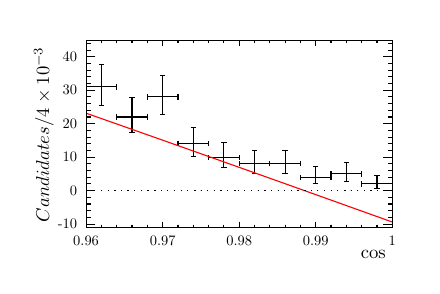
\begin{tikzpicture}
\pgfdeclareplotmark{cross} {
\pgfpathmoveto{\pgfpoint{-0.3\pgfplotmarksize}{\pgfplotmarksize}}
\pgfpathlineto{\pgfpoint{+0.3\pgfplotmarksize}{\pgfplotmarksize}}
\pgfpathlineto{\pgfpoint{+0.3\pgfplotmarksize}{0.3\pgfplotmarksize}}
\pgfpathlineto{\pgfpoint{+1\pgfplotmarksize}{0.3\pgfplotmarksize}}
\pgfpathlineto{\pgfpoint{+1\pgfplotmarksize}{-0.3\pgfplotmarksize}}
\pgfpathlineto{\pgfpoint{+0.3\pgfplotmarksize}{-0.3\pgfplotmarksize}}
\pgfpathlineto{\pgfpoint{+0.3\pgfplotmarksize}{-1.\pgfplotmarksize}}
\pgfpathlineto{\pgfpoint{-0.3\pgfplotmarksize}{-1.\pgfplotmarksize}}
\pgfpathlineto{\pgfpoint{-0.3\pgfplotmarksize}{-0.3\pgfplotmarksize}}
\pgfpathlineto{\pgfpoint{-1.\pgfplotmarksize}{-0.3\pgfplotmarksize}}
\pgfpathlineto{\pgfpoint{-1.\pgfplotmarksize}{0.3\pgfplotmarksize}}
\pgfpathlineto{\pgfpoint{-0.3\pgfplotmarksize}{0.3\pgfplotmarksize}}
\pgfpathclose
\pgfusepathqstroke
}
\pgfdeclareplotmark{cross*} {
\pgfpathmoveto{\pgfpoint{-0.3\pgfplotmarksize}{\pgfplotmarksize}}
\pgfpathlineto{\pgfpoint{+0.3\pgfplotmarksize}{\pgfplotmarksize}}
\pgfpathlineto{\pgfpoint{+0.3\pgfplotmarksize}{0.3\pgfplotmarksize}}
\pgfpathlineto{\pgfpoint{+1\pgfplotmarksize}{0.3\pgfplotmarksize}}
\pgfpathlineto{\pgfpoint{+1\pgfplotmarksize}{-0.3\pgfplotmarksize}}
\pgfpathlineto{\pgfpoint{+0.3\pgfplotmarksize}{-0.3\pgfplotmarksize}}
\pgfpathlineto{\pgfpoint{+0.3\pgfplotmarksize}{-1.\pgfplotmarksize}}
\pgfpathlineto{\pgfpoint{-0.3\pgfplotmarksize}{-1.\pgfplotmarksize}}
\pgfpathlineto{\pgfpoint{-0.3\pgfplotmarksize}{-0.3\pgfplotmarksize}}
\pgfpathlineto{\pgfpoint{-1.\pgfplotmarksize}{-0.3\pgfplotmarksize}}
\pgfpathlineto{\pgfpoint{-1.\pgfplotmarksize}{0.3\pgfplotmarksize}}
\pgfpathlineto{\pgfpoint{-0.3\pgfplotmarksize}{0.3\pgfplotmarksize}}
\pgfpathclose
\pgfusepathqfillstroke
}
\pgfdeclareplotmark{newstar} {
\pgfpathmoveto{\pgfqpoint{0pt}{\pgfplotmarksize}}
\pgfpathlineto{\pgfqpointpolar{44}{0.5\pgfplotmarksize}}
\pgfpathlineto{\pgfqpointpolar{18}{\pgfplotmarksize}}
\pgfpathlineto{\pgfqpointpolar{-20}{0.5\pgfplotmarksize}}
\pgfpathlineto{\pgfqpointpolar{-54}{\pgfplotmarksize}}
\pgfpathlineto{\pgfqpointpolar{-90}{0.5\pgfplotmarksize}}
\pgfpathlineto{\pgfqpointpolar{234}{\pgfplotmarksize}}
\pgfpathlineto{\pgfqpointpolar{198}{0.5\pgfplotmarksize}}
\pgfpathlineto{\pgfqpointpolar{162}{\pgfplotmarksize}}
\pgfpathlineto{\pgfqpointpolar{134}{0.5\pgfplotmarksize}}
\pgfpathclose
\pgfusepathqstroke
}
\pgfdeclareplotmark{newstar*} {
\pgfpathmoveto{\pgfqpoint{0pt}{\pgfplotmarksize}}
\pgfpathlineto{\pgfqpointpolar{44}{0.5\pgfplotmarksize}}
\pgfpathlineto{\pgfqpointpolar{18}{\pgfplotmarksize}}
\pgfpathlineto{\pgfqpointpolar{-20}{0.5\pgfplotmarksize}}
\pgfpathlineto{\pgfqpointpolar{-54}{\pgfplotmarksize}}
\pgfpathlineto{\pgfqpointpolar{-90}{0.5\pgfplotmarksize}}
\pgfpathlineto{\pgfqpointpolar{234}{\pgfplotmarksize}}
\pgfpathlineto{\pgfqpointpolar{198}{0.5\pgfplotmarksize}}
\pgfpathlineto{\pgfqpointpolar{162}{\pgfplotmarksize}}
\pgfpathlineto{\pgfqpointpolar{134}{0.5\pgfplotmarksize}}
\pgfpathclose
\pgfusepathqfillstroke
}
\definecolor{c}{rgb}{1,1,1};
\draw [color=c, fill=c] (0.1,3.20034) rectangle (4.9,6.21242);
\draw [color=c, fill=c] (0.772,3.68227) rectangle (4.66,6.06181);
\definecolor{c}{rgb}{0,0,0};
\draw [c] (0.772,3.68227) -- (0.772,6.06181) -- (4.66,6.06181) -- (4.66,3.68227) -- (0.772,3.68227);
\draw [c,line width=0.4] (0.772,3.68227) -- (4.66,3.68227);
\draw [anchor= east] (4.66,3.34492) node[scale=0.672711, rotate=0]{$\cos\thetaK$};
\draw [c,line width=0.4] (0.772,3.75546) -- (0.772,3.68227);
\draw [c,line width=0.4] (0.9664,3.71887) -- (0.9664,3.68227);
\draw [c,line width=0.4] (1.1608,3.71887) -- (1.1608,3.68227);
\draw [c,line width=0.4] (1.3552,3.71887) -- (1.3552,3.68227);
\draw [c,line width=0.4] (1.5496,3.71887) -- (1.5496,3.68227);
\draw [c,line width=0.4] (1.744,3.75546) -- (1.744,3.68227);
\draw [c,line width=0.4] (1.9384,3.71887) -- (1.9384,3.68227);
\draw [c,line width=0.4] (2.1328,3.71887) -- (2.1328,3.68227);
\draw [c,line width=0.4] (2.3272,3.71887) -- (2.3272,3.68227);
\draw [c,line width=0.4] (2.5216,3.71887) -- (2.5216,3.68227);
\draw [c,line width=0.4] (2.716,3.75546) -- (2.716,3.68227);
\draw [c,line width=0.4] (2.9104,3.71887) -- (2.9104,3.68227);
\draw [c,line width=0.4] (3.1048,3.71887) -- (3.1048,3.68227);
\draw [c,line width=0.4] (3.2992,3.71887) -- (3.2992,3.68227);
\draw [c,line width=0.4] (3.4936,3.71887) -- (3.4936,3.68227);
\draw [c,line width=0.4] (3.688,3.75546) -- (3.688,3.68227);
\draw [c,line width=0.4] (3.8824,3.71887) -- (3.8824,3.68227);
\draw [c,line width=0.4] (4.0768,3.71887) -- (4.0768,3.68227);
\draw [c,line width=0.4] (4.2712,3.71887) -- (4.2712,3.68227);
\draw [c,line width=0.4] (4.4656,3.71887) -- (4.4656,3.68227);
\draw [c,line width=0.4] (4.66,3.75546) -- (4.66,3.68227);
\draw [anchor=base] (0.772,3.45937) node[scale=0.52322, rotate=0]{0.96};
\draw [anchor=base] (1.744,3.45937) node[scale=0.52322, rotate=0]{0.97};
\draw [anchor=base] (2.716,3.45937) node[scale=0.52322, rotate=0]{0.98};
\draw [anchor=base] (3.688,3.45937) node[scale=0.52322, rotate=0]{0.99};
\draw [anchor=base] (4.66,3.45937) node[scale=0.52322, rotate=0]{1};
\draw [c,line width=0.4] (0.772,6.06181) -- (4.66,6.06181);
\draw [c,line width=0.4] (0.772,5.98862) -- (0.772,6.06181);
\draw [c,line width=0.4] (0.9664,6.02522) -- (0.9664,6.06181);
\draw [c,line width=0.4] (1.1608,6.02522) -- (1.1608,6.06181);
\draw [c,line width=0.4] (1.3552,6.02522) -- (1.3552,6.06181);
\draw [c,line width=0.4] (1.5496,6.02522) -- (1.5496,6.06181);
\draw [c,line width=0.4] (1.744,5.98862) -- (1.744,6.06181);
\draw [c,line width=0.4] (1.9384,6.02522) -- (1.9384,6.06181);
\draw [c,line width=0.4] (2.1328,6.02522) -- (2.1328,6.06181);
\draw [c,line width=0.4] (2.3272,6.02522) -- (2.3272,6.06181);
\draw [c,line width=0.4] (2.5216,6.02522) -- (2.5216,6.06181);
\draw [c,line width=0.4] (2.716,5.98862) -- (2.716,6.06181);
\draw [c,line width=0.4] (2.9104,6.02522) -- (2.9104,6.06181);
\draw [c,line width=0.4] (3.1048,6.02522) -- (3.1048,6.06181);
\draw [c,line width=0.4] (3.2992,6.02522) -- (3.2992,6.06181);
\draw [c,line width=0.4] (3.4936,6.02522) -- (3.4936,6.06181);
\draw [c,line width=0.4] (3.688,5.98862) -- (3.688,6.06181);
\draw [c,line width=0.4] (3.8824,6.02522) -- (3.8824,6.06181);
\draw [c,line width=0.4] (4.0768,6.02522) -- (4.0768,6.06181);
\draw [c,line width=0.4] (4.2712,6.02522) -- (4.2712,6.06181);
\draw [c,line width=0.4] (4.4656,6.02522) -- (4.4656,6.06181);
\draw [c,line width=0.4] (4.66,5.98862) -- (4.66,6.06181);
\draw [c,line width=0.4] (0.772,3.68227) -- (0.772,6.06181);
\draw [anchor= east] (0.2344,6.06181) node[scale=0.672711, rotate=90]{$\text{Candidates} / 4\times10^{-3}$};
\draw [c,line width=0.4] (0.88576,3.72536) -- (0.772,3.72536);
\draw [c,line width=0.4] (0.82888,3.81032) -- (0.772,3.81032);
\draw [c,line width=0.4] (0.82888,3.89528) -- (0.772,3.89528);
\draw [c,line width=0.4] (0.82888,3.98024) -- (0.772,3.98024);
\draw [c,line width=0.4] (0.82888,4.06521) -- (0.772,4.06521);
\draw [c,line width=0.4] (0.88576,4.15017) -- (0.772,4.15017);
\draw [c,line width=0.4] (0.82888,4.23513) -- (0.772,4.23513);
\draw [c,line width=0.4] (0.82888,4.32009) -- (0.772,4.32009);
\draw [c,line width=0.4] (0.82888,4.40505) -- (0.772,4.40505);
\draw [c,line width=0.4] (0.82888,4.49002) -- (0.772,4.49002);
\draw [c,line width=0.4] (0.88576,4.57498) -- (0.772,4.57498);
\draw [c,line width=0.4] (0.82888,4.65994) -- (0.772,4.65994);
\draw [c,line width=0.4] (0.82888,4.7449) -- (0.772,4.7449);
\draw [c,line width=0.4] (0.82888,4.82986) -- (0.772,4.82986);
\draw [c,line width=0.4] (0.82888,4.91482) -- (0.772,4.91482);
\draw [c,line width=0.4] (0.88576,4.99979) -- (0.772,4.99979);
\draw [c,line width=0.4] (0.82888,5.08475) -- (0.772,5.08475);
\draw [c,line width=0.4] (0.82888,5.16971) -- (0.772,5.16971);
\draw [c,line width=0.4] (0.82888,5.25467) -- (0.772,5.25467);
\draw [c,line width=0.4] (0.82888,5.33964) -- (0.772,5.33964);
\draw [c,line width=0.4] (0.88576,5.4246) -- (0.772,5.4246);
\draw [c,line width=0.4] (0.82888,5.50956) -- (0.772,5.50956);
\draw [c,line width=0.4] (0.82888,5.59452) -- (0.772,5.59452);
\draw [c,line width=0.4] (0.82888,5.67948) -- (0.772,5.67948);
\draw [c,line width=0.4] (0.82888,5.76445) -- (0.772,5.76445);
\draw [c,line width=0.4] (0.88576,5.84941) -- (0.772,5.84941);
\draw [c,line width=0.4] (0.88576,3.72536) -- (0.772,3.72536);
\draw [c,line width=0.4] (0.88576,5.84941) -- (0.772,5.84941);
\draw [c,line width=0.4] (0.82888,5.93437) -- (0.772,5.93437);
\draw [c,line width=0.4] (0.82888,6.01933) -- (0.772,6.01933);
\draw [anchor= east] (0.724,3.72536) node[scale=0.52322, rotate=0]{-10};
\draw [anchor= east] (0.724,4.15017) node[scale=0.52322, rotate=0]{0};
\draw [anchor= east] (0.724,4.57498) node[scale=0.52322, rotate=0]{10};
\draw [anchor= east] (0.724,4.99979) node[scale=0.52322, rotate=0]{20};
\draw [anchor= east] (0.724,5.4246) node[scale=0.52322, rotate=0]{30};
\draw [anchor= east] (0.724,5.84941) node[scale=0.52322, rotate=0]{40};
\draw [c,line width=0.4] (4.66,3.68227) -- (4.66,6.06181);
\draw [c,line width=0.4] (4.54624,3.72536) -- (4.66,3.72536);
\draw [c,line width=0.4] (4.60312,3.81032) -- (4.66,3.81032);
\draw [c,line width=0.4] (4.60312,3.89528) -- (4.66,3.89528);
\draw [c,line width=0.4] (4.60312,3.98024) -- (4.66,3.98024);
\draw [c,line width=0.4] (4.60312,4.06521) -- (4.66,4.06521);
\draw [c,line width=0.4] (4.54624,4.15017) -- (4.66,4.15017);
\draw [c,line width=0.4] (4.60312,4.23513) -- (4.66,4.23513);
\draw [c,line width=0.4] (4.60312,4.32009) -- (4.66,4.32009);
\draw [c,line width=0.4] (4.60312,4.40505) -- (4.66,4.40505);
\draw [c,line width=0.4] (4.60312,4.49002) -- (4.66,4.49002);
\draw [c,line width=0.4] (4.54624,4.57498) -- (4.66,4.57498);
\draw [c,line width=0.4] (4.60312,4.65994) -- (4.66,4.65994);
\draw [c,line width=0.4] (4.60312,4.7449) -- (4.66,4.7449);
\draw [c,line width=0.4] (4.60312,4.82986) -- (4.66,4.82986);
\draw [c,line width=0.4] (4.60312,4.91482) -- (4.66,4.91482);
\draw [c,line width=0.4] (4.54624,4.99979) -- (4.66,4.99979);
\draw [c,line width=0.4] (4.60312,5.08475) -- (4.66,5.08475);
\draw [c,line width=0.4] (4.60312,5.16971) -- (4.66,5.16971);
\draw [c,line width=0.4] (4.60312,5.25467) -- (4.66,5.25467);
\draw [c,line width=0.4] (4.60312,5.33964) -- (4.66,5.33964);
\draw [c,line width=0.4] (4.54624,5.4246) -- (4.66,5.4246);
\draw [c,line width=0.4] (4.60312,5.50956) -- (4.66,5.50956);
\draw [c,line width=0.4] (4.60312,5.59452) -- (4.66,5.59452);
\draw [c,line width=0.4] (4.60312,5.67948) -- (4.66,5.67948);
\draw [c,line width=0.4] (4.60312,5.76445) -- (4.66,5.76445);
\draw [c,line width=0.4] (4.54624,5.84941) -- (4.66,5.84941);
\draw [c,line width=0.4] (4.54624,3.72536) -- (4.66,3.72536);
\draw [c,line width=0.4] (4.54624,5.84941) -- (4.66,5.84941);
\draw [c,line width=0.4] (4.60312,5.93437) -- (4.66,5.93437);
\draw [c,line width=0.4] (4.60312,6.01933) -- (4.66,6.01933);
\draw [c,line width=0.4] (0.9664,5.46708) -- (0.772,5.46708);
\draw [c,line width=0.4] (0.772,5.43352) -- (0.772,5.50064);
\draw [c,line width=0.4] (0.9664,5.46708) -- (1.1608,5.46708);
\draw [c,line width=0.4] (1.1608,5.43352) -- (1.1608,5.50064);
\draw [c,line width=0.4] (0.9664,5.46708) -- (0.9664,5.74863);
\draw [c,line width=0.4] (0.932843,5.74863) -- (0.999957,5.74863);
\draw [c,line width=0.4] (0.9664,5.46708) -- (0.9664,5.23184);
\draw [c,line width=0.4] (0.932843,5.23184) -- (0.999957,5.23184);
\draw [c,line width=0.4] (1.3552,5.08475) -- (1.1608,5.08475);
\draw [c,line width=0.4] (1.1608,5.05119) -- (1.1608,5.11831);
\draw [c,line width=0.4] (1.3552,5.08475) -- (1.5496,5.08475);
\draw [c,line width=0.4] (1.5496,5.05119) -- (1.5496,5.11831);
\draw [c,line width=0.4] (1.3552,5.08475) -- (1.3552,5.3295);
\draw [c,line width=0.4] (1.32164,5.3295) -- (1.38876,5.3295);
\draw [c,line width=0.4] (1.3552,5.08475) -- (1.3552,4.88702);
\draw [c,line width=0.4] (1.32164,4.88702) -- (1.38876,4.88702);
\draw [c,line width=0.4] (1.744,5.33964) -- (1.5496,5.33964);
\draw [c,line width=0.4] (1.5496,5.30608) -- (1.5496,5.37319);
\draw [c,line width=0.4] (1.744,5.33964) -- (1.9384,5.33964);
\draw [c,line width=0.4] (1.9384,5.30608) -- (1.9384,5.37319);
\draw [c,line width=0.4] (1.744,5.33964) -- (1.744,5.60958);
\draw [c,line width=0.4] (1.71044,5.60958) -- (1.77756,5.60958);
\draw [c,line width=0.4] (1.744,5.33964) -- (1.744,5.1162);
\draw [c,line width=0.4] (1.71044,5.1162) -- (1.77756,5.1162);
\draw [c,line width=0.4] (2.1328,4.7449) -- (1.9384,4.7449);
\draw [c,line width=0.4] (1.9384,4.71134) -- (1.9384,4.77846);
\draw [c,line width=0.4] (2.1328,4.7449) -- (2.3272,4.7449);
\draw [c,line width=0.4] (2.3272,4.71134) -- (2.3272,4.77846);
\draw [c,line width=0.4] (2.1328,4.7449) -- (2.1328,4.9501);
\draw [c,line width=0.4] (2.09924,4.9501) -- (2.16636,4.9501);
\draw [c,line width=0.4] (2.1328,4.7449) -- (2.1328,4.58787);
\draw [c,line width=0.4] (2.09924,4.58787) -- (2.16636,4.58787);
\draw [c,line width=0.4] (2.5216,4.57498) -- (2.3272,4.57498);
\draw [c,line width=0.4] (2.3272,4.54142) -- (2.3272,4.60853);
\draw [c,line width=0.4] (2.5216,4.57498) -- (2.716,4.57498);
\draw [c,line width=0.4] (2.716,4.54142) -- (2.716,4.60853);
\draw [c,line width=0.4] (2.5216,4.57498) -- (2.5216,4.75624);
\draw [c,line width=0.4] (2.48804,4.75624) -- (2.55516,4.75624);
\draw [c,line width=0.4] (2.5216,4.57498) -- (2.5216,4.44292);
\draw [c,line width=0.4] (2.48804,4.44292) -- (2.55516,4.44292);
\draw [c,line width=0.4] (2.9104,4.49002) -- (2.716,4.49002);
\draw [c,line width=0.4] (2.716,4.45646) -- (2.716,4.52357);
\draw [c,line width=0.4] (2.9104,4.49002) -- (3.1048,4.49002);
\draw [c,line width=0.4] (3.1048,4.45646) -- (3.1048,4.52357);
\draw [c,line width=0.4] (2.9104,4.49002) -- (2.9104,4.65761);
\draw [c,line width=0.4] (2.87684,4.65761) -- (2.94396,4.65761);
\draw [c,line width=0.4] (2.9104,4.49002) -- (2.9104,4.37241);
\draw [c,line width=0.4] (2.87684,4.37241) -- (2.94396,4.37241);
\draw [c,line width=0.4] (3.2992,4.49002) -- (3.1048,4.49002);
\draw [c,line width=0.4] (3.1048,4.45646) -- (3.1048,4.52357);
\draw [c,line width=0.4] (3.2992,4.49002) -- (3.4936,4.49002);
\draw [c,line width=0.4] (3.4936,4.45646) -- (3.4936,4.52357);
\draw [c,line width=0.4] (3.2992,4.49002) -- (3.2992,4.65761);
\draw [c,line width=0.4] (3.26564,4.65761) -- (3.33276,4.65761);
\draw [c,line width=0.4] (3.2992,4.49002) -- (3.2992,4.37241);
\draw [c,line width=0.4] (3.26564,4.37241) -- (3.33276,4.37241);
\draw [c,line width=0.4] (3.688,4.32009) -- (3.4936,4.32009);
\draw [c,line width=0.4] (3.4936,4.28653) -- (3.4936,4.35365);
\draw [c,line width=0.4] (3.688,4.32009) -- (3.8824,4.32009);
\draw [c,line width=0.4] (3.8824,4.28653) -- (3.8824,4.35365);
\draw [c,line width=0.4] (3.688,4.32009) -- (3.688,4.45445);
\draw [c,line width=0.4] (3.65444,4.45445) -- (3.72156,4.45445);
\draw [c,line width=0.4] (3.688,4.32009) -- (3.688,4.23877);
\draw [c,line width=0.4] (3.65444,4.23877) -- (3.72156,4.23877);
\draw [c,line width=0.4] (4.0768,4.36257) -- (3.8824,4.36257);
\draw [c,line width=0.4] (3.8824,4.32901) -- (3.8824,4.39613);
\draw [c,line width=0.4] (4.0768,4.36257) -- (4.2712,4.36257);
\draw [c,line width=0.4] (4.2712,4.32901) -- (4.2712,4.39613);
\draw [c,line width=0.4] (4.0768,4.36257) -- (4.0768,4.50626);
\draw [c,line width=0.4] (4.04324,4.50626) -- (4.11036,4.50626);
\draw [c,line width=0.4] (4.0768,4.36257) -- (4.0768,4.27083);
\draw [c,line width=0.4] (4.04324,4.27083) -- (4.11036,4.27083);
\draw [c,line width=0.4] (4.4656,4.23513) -- (4.2712,4.23513);
\draw [c,line width=0.4] (4.2712,4.20157) -- (4.2712,4.26869);
\draw [c,line width=0.4] (4.4656,4.23513) -- (4.66,4.23513);
\draw [c,line width=0.4] (4.66,4.20157) -- (4.66,4.26869);
\draw [c,line width=0.4] (4.4656,4.23513) -- (4.4656,4.34719);
\draw [c,line width=0.4] (4.43204,4.34719) -- (4.49916,4.34719);
\draw [c,line width=0.4] (4.4656,4.23513) -- (4.4656,4.18025);
\draw [c,line width=0.4] (4.43204,4.18025) -- (4.49916,4.18025);
\foreach \P in {(0.9664,5.46708),(1.3552,5.08475),(1.744,5.33964),(2.1328,4.7449),(2.5216,4.57498),(2.9104,4.49002),(3.2992,4.49002),(3.688,4.32009),(4.0768,4.36257),(4.4656,4.23513)}{\draw[mark options={color=c,fill=c},mark size=0.960961pt,mark=]
 plot coordinates {\P};}
\definecolor{c}{rgb}{1,0,0};
\draw [c,line width=0.4] (0.772,5.13337) -- (0.772,5.13337);
\draw [c,line width=0.4] (0.772,5.13337) -- (1.1608,4.99651) -- (1.5496,4.85928) -- (1.9384,4.72173) -- (2.3272,4.58385) -- (2.716,4.44569) -- (3.1048,4.30726) -- (3.4936,4.16858) -- (3.8824,4.02969) -- (4.2712,3.89061) -- (4.66,3.75137) --
 (4.66,3.75137) -- (4.66,3.75137);
\definecolor{c}{rgb}{0,0,0};
\draw [c,line width=0.4] (0.772,3.68227) -- (4.66,3.68227);
\draw [c,line width=0.4] (0.772,3.75546) -- (0.772,3.68227);
\draw [c,line width=0.4] (0.9664,3.71887) -- (0.9664,3.68227);
\draw [c,line width=0.4] (1.1608,3.71887) -- (1.1608,3.68227);
\draw [c,line width=0.4] (1.3552,3.71887) -- (1.3552,3.68227);
\draw [c,line width=0.4] (1.5496,3.71887) -- (1.5496,3.68227);
\draw [c,line width=0.4] (1.744,3.75546) -- (1.744,3.68227);
\draw [c,line width=0.4] (1.9384,3.71887) -- (1.9384,3.68227);
\draw [c,line width=0.4] (2.1328,3.71887) -- (2.1328,3.68227);
\draw [c,line width=0.4] (2.3272,3.71887) -- (2.3272,3.68227);
\draw [c,line width=0.4] (2.5216,3.71887) -- (2.5216,3.68227);
\draw [c,line width=0.4] (2.716,3.75546) -- (2.716,3.68227);
\draw [c,line width=0.4] (2.9104,3.71887) -- (2.9104,3.68227);
\draw [c,line width=0.4] (3.1048,3.71887) -- (3.1048,3.68227);
\draw [c,line width=0.4] (3.2992,3.71887) -- (3.2992,3.68227);
\draw [c,line width=0.4] (3.4936,3.71887) -- (3.4936,3.68227);
\draw [c,line width=0.4] (3.688,3.75546) -- (3.688,3.68227);
\draw [c,line width=0.4] (3.8824,3.71887) -- (3.8824,3.68227);
\draw [c,line width=0.4] (4.0768,3.71887) -- (4.0768,3.68227);
\draw [c,line width=0.4] (4.2712,3.71887) -- (4.2712,3.68227);
\draw [c,line width=0.4] (4.4656,3.71887) -- (4.4656,3.68227);
\draw [c,line width=0.4] (4.66,3.75546) -- (4.66,3.68227);
\draw [c,line width=0.4] (0.772,6.06181) -- (4.66,6.06181);
\draw [c,line width=0.4] (0.772,5.98862) -- (0.772,6.06181);
\draw [c,line width=0.4] (0.9664,6.02522) -- (0.9664,6.06181);
\draw [c,line width=0.4] (1.1608,6.02522) -- (1.1608,6.06181);
\draw [c,line width=0.4] (1.3552,6.02522) -- (1.3552,6.06181);
\draw [c,line width=0.4] (1.5496,6.02522) -- (1.5496,6.06181);
\draw [c,line width=0.4] (1.744,5.98862) -- (1.744,6.06181);
\draw [c,line width=0.4] (1.9384,6.02522) -- (1.9384,6.06181);
\draw [c,line width=0.4] (2.1328,6.02522) -- (2.1328,6.06181);
\draw [c,line width=0.4] (2.3272,6.02522) -- (2.3272,6.06181);
\draw [c,line width=0.4] (2.5216,6.02522) -- (2.5216,6.06181);
\draw [c,line width=0.4] (2.716,5.98862) -- (2.716,6.06181);
\draw [c,line width=0.4] (2.9104,6.02522) -- (2.9104,6.06181);
\draw [c,line width=0.4] (3.1048,6.02522) -- (3.1048,6.06181);
\draw [c,line width=0.4] (3.2992,6.02522) -- (3.2992,6.06181);
\draw [c,line width=0.4] (3.4936,6.02522) -- (3.4936,6.06181);
\draw [c,line width=0.4] (3.688,5.98862) -- (3.688,6.06181);
\draw [c,line width=0.4] (3.8824,6.02522) -- (3.8824,6.06181);
\draw [c,line width=0.4] (4.0768,6.02522) -- (4.0768,6.06181);
\draw [c,line width=0.4] (4.2712,6.02522) -- (4.2712,6.06181);
\draw [c,line width=0.4] (4.4656,6.02522) -- (4.4656,6.06181);
\draw [c,line width=0.4] (4.66,5.98862) -- (4.66,6.06181);
\draw [c,line width=0.4] (0.772,3.68227) -- (0.772,6.06181);
\draw [c,line width=0.4] (0.88576,3.72536) -- (0.772,3.72536);
\draw [c,line width=0.4] (0.82888,3.81032) -- (0.772,3.81032);
\draw [c,line width=0.4] (0.82888,3.89528) -- (0.772,3.89528);
\draw [c,line width=0.4] (0.82888,3.98024) -- (0.772,3.98024);
\draw [c,line width=0.4] (0.82888,4.06521) -- (0.772,4.06521);
\draw [c,line width=0.4] (0.88576,4.15017) -- (0.772,4.15017);
\draw [c,line width=0.4] (0.82888,4.23513) -- (0.772,4.23513);
\draw [c,line width=0.4] (0.82888,4.32009) -- (0.772,4.32009);
\draw [c,line width=0.4] (0.82888,4.40505) -- (0.772,4.40505);
\draw [c,line width=0.4] (0.82888,4.49002) -- (0.772,4.49002);
\draw [c,line width=0.4] (0.88576,4.57498) -- (0.772,4.57498);
\draw [c,line width=0.4] (0.82888,4.65994) -- (0.772,4.65994);
\draw [c,line width=0.4] (0.82888,4.7449) -- (0.772,4.7449);
\draw [c,line width=0.4] (0.82888,4.82986) -- (0.772,4.82986);
\draw [c,line width=0.4] (0.82888,4.91482) -- (0.772,4.91482);
\draw [c,line width=0.4] (0.88576,4.99979) -- (0.772,4.99979);
\draw [c,line width=0.4] (0.82888,5.08475) -- (0.772,5.08475);
\draw [c,line width=0.4] (0.82888,5.16971) -- (0.772,5.16971);
\draw [c,line width=0.4] (0.82888,5.25467) -- (0.772,5.25467);
\draw [c,line width=0.4] (0.82888,5.33964) -- (0.772,5.33964);
\draw [c,line width=0.4] (0.88576,5.4246) -- (0.772,5.4246);
\draw [c,line width=0.4] (0.82888,5.50956) -- (0.772,5.50956);
\draw [c,line width=0.4] (0.82888,5.59452) -- (0.772,5.59452);
\draw [c,line width=0.4] (0.82888,5.67948) -- (0.772,5.67948);
\draw [c,line width=0.4] (0.82888,5.76445) -- (0.772,5.76445);
\draw [c,line width=0.4] (0.88576,5.84941) -- (0.772,5.84941);
\draw [c,line width=0.4] (0.88576,3.72536) -- (0.772,3.72536);
\draw [c,line width=0.4] (0.88576,5.84941) -- (0.772,5.84941);
\draw [c,line width=0.4] (0.82888,5.93437) -- (0.772,5.93437);
\draw [c,line width=0.4] (0.82888,6.01933) -- (0.772,6.01933);
\draw [c,line width=0.4] (4.66,3.68227) -- (4.66,6.06181);
\draw [c,line width=0.4] (4.54624,3.72536) -- (4.66,3.72536);
\draw [c,line width=0.4] (4.60312,3.81032) -- (4.66,3.81032);
\draw [c,line width=0.4] (4.60312,3.89528) -- (4.66,3.89528);
\draw [c,line width=0.4] (4.60312,3.98024) -- (4.66,3.98024);
\draw [c,line width=0.4] (4.60312,4.06521) -- (4.66,4.06521);
\draw [c,line width=0.4] (4.54624,4.15017) -- (4.66,4.15017);
\draw [c,line width=0.4] (4.60312,4.23513) -- (4.66,4.23513);
\draw [c,line width=0.4] (4.60312,4.32009) -- (4.66,4.32009);
\draw [c,line width=0.4] (4.60312,4.40505) -- (4.66,4.40505);
\draw [c,line width=0.4] (4.60312,4.49002) -- (4.66,4.49002);
\draw [c,line width=0.4] (4.54624,4.57498) -- (4.66,4.57498);
\draw [c,line width=0.4] (4.60312,4.65994) -- (4.66,4.65994);
\draw [c,line width=0.4] (4.60312,4.7449) -- (4.66,4.7449);
\draw [c,line width=0.4] (4.60312,4.82986) -- (4.66,4.82986);
\draw [c,line width=0.4] (4.60312,4.91482) -- (4.66,4.91482);
\draw [c,line width=0.4] (4.54624,4.99979) -- (4.66,4.99979);
\draw [c,line width=0.4] (4.60312,5.08475) -- (4.66,5.08475);
\draw [c,line width=0.4] (4.60312,5.16971) -- (4.66,5.16971);
\draw [c,line width=0.4] (4.60312,5.25467) -- (4.66,5.25467);
\draw [c,line width=0.4] (4.60312,5.33964) -- (4.66,5.33964);
\draw [c,line width=0.4] (4.54624,5.4246) -- (4.66,5.4246);
\draw [c,line width=0.4] (4.60312,5.50956) -- (4.66,5.50956);
\draw [c,line width=0.4] (4.60312,5.59452) -- (4.66,5.59452);
\draw [c,line width=0.4] (4.60312,5.67948) -- (4.66,5.67948);
\draw [c,line width=0.4] (4.60312,5.76445) -- (4.66,5.76445);
\draw [c,line width=0.4] (4.54624,5.84941) -- (4.66,5.84941);
\draw [c,line width=0.4] (4.54624,3.72536) -- (4.66,3.72536);
\draw [c,line width=0.4] (4.54624,5.84941) -- (4.66,5.84941);
\draw [c,line width=0.4] (4.60312,5.93437) -- (4.66,5.93437);
\draw [c,line width=0.4] (4.60312,6.01933) -- (4.66,6.01933);
\draw [c,dotted,line width=0.4] (0.79144,4.15017) -- (0.83032,4.15017) -- (0.8692,4.15017) -- (0.90808,4.15017) -- (0.94696,4.15017) -- (0.98584,4.15017) -- (1.02472,4.15017) -- (1.0636,4.15017) -- (1.10248,4.15017) -- (1.14136,4.15017) --
 (1.18024,4.15017) -- (1.21912,4.15017) -- (1.258,4.15017) -- (1.29688,4.15017) -- (1.33576,4.15017) -- (1.37464,4.15017) -- (1.41352,4.15017) -- (1.4524,4.15017) -- (1.49128,4.15017) -- (1.53016,4.15017) -- (1.56904,4.15017) -- (1.60792,4.15017) --
 (1.6468,4.15017) -- (1.68568,4.15017) -- (1.72456,4.15017) -- (1.76344,4.15017) -- (1.80232,4.15017) -- (1.8412,4.15017) -- (1.88008,4.15017) -- (1.91896,4.15017) -- (1.95784,4.15017) -- (1.99672,4.15017) -- (2.0356,4.15017) -- (2.07448,4.15017) --
 (2.11336,4.15017) -- (2.15224,4.15017) -- (2.19112,4.15017) -- (2.23,4.15017) -- (2.26888,4.15017) -- (2.30776,4.15017) -- (2.34664,4.15017) -- (2.38552,4.15017) -- (2.4244,4.15017) -- (2.46328,4.15017) -- (2.50216,4.15017) -- (2.54104,4.15017) --
 (2.57992,4.15017) -- (2.6188,4.15017) -- (2.65768,4.15017) -- (2.69656,4.15017);
\draw [c,dotted,line width=0.4] (2.69656,4.15017) -- (2.73544,4.15017) -- (2.77432,4.15017) -- (2.8132,4.15017) -- (2.85208,4.15017) -- (2.89096,4.15017) -- (2.92984,4.15017) -- (2.96872,4.15017) -- (3.0076,4.15017) -- (3.04648,4.15017) --
 (3.08536,4.15017) -- (3.12424,4.15017) -- (3.16312,4.15017) -- (3.202,4.15017) -- (3.24088,4.15017) -- (3.27976,4.15017) -- (3.31864,4.15017) -- (3.35752,4.15017) -- (3.3964,4.15017) -- (3.43528,4.15017) -- (3.47416,4.15017) -- (3.51304,4.15017) --
 (3.55192,4.15017) -- (3.5908,4.15017) -- (3.62968,4.15017) -- (3.66856,4.15017) -- (3.70744,4.15017) -- (3.74632,4.15017) -- (3.7852,4.15017) -- (3.82408,4.15017) -- (3.86296,4.15017) -- (3.90184,4.15017) -- (3.94072,4.15017) -- (3.9796,4.15017) --
 (4.01848,4.15017) -- (4.05736,4.15017) -- (4.09624,4.15017) -- (4.13512,4.15017) -- (4.174,4.15017) -- (4.21288,4.15017) -- (4.25176,4.15017) -- (4.29064,4.15017) -- (4.32952,4.15017) -- (4.3684,4.15017) -- (4.40728,4.15017) -- (4.44616,4.15017) --
 (4.48504,4.15017) -- (4.52392,4.15017) -- (4.5628,4.15017) -- (4.60168,4.15017);
\draw [c,dotted,line width=0.4] (4.60168,4.15017) -- (4.64056,4.15017);
\end{tikzpicture}
}
    \caption{}
    \label{angAcc_nom}
  \end{subfigure}%
  \hfill%
  \begin{subfigure}{0.5\textwidth}
    \tikzsetnextfilename{eff_helcosthetaK_neg_all_constr_fit_zoom}
    \scalebox{1.3}{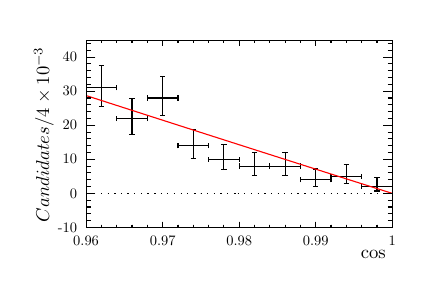
\begin{tikzpicture}
\pgfdeclareplotmark{cross} {
\pgfpathmoveto{\pgfpoint{-0.3\pgfplotmarksize}{\pgfplotmarksize}}
\pgfpathlineto{\pgfpoint{+0.3\pgfplotmarksize}{\pgfplotmarksize}}
\pgfpathlineto{\pgfpoint{+0.3\pgfplotmarksize}{0.3\pgfplotmarksize}}
\pgfpathlineto{\pgfpoint{+1\pgfplotmarksize}{0.3\pgfplotmarksize}}
\pgfpathlineto{\pgfpoint{+1\pgfplotmarksize}{-0.3\pgfplotmarksize}}
\pgfpathlineto{\pgfpoint{+0.3\pgfplotmarksize}{-0.3\pgfplotmarksize}}
\pgfpathlineto{\pgfpoint{+0.3\pgfplotmarksize}{-1.\pgfplotmarksize}}
\pgfpathlineto{\pgfpoint{-0.3\pgfplotmarksize}{-1.\pgfplotmarksize}}
\pgfpathlineto{\pgfpoint{-0.3\pgfplotmarksize}{-0.3\pgfplotmarksize}}
\pgfpathlineto{\pgfpoint{-1.\pgfplotmarksize}{-0.3\pgfplotmarksize}}
\pgfpathlineto{\pgfpoint{-1.\pgfplotmarksize}{0.3\pgfplotmarksize}}
\pgfpathlineto{\pgfpoint{-0.3\pgfplotmarksize}{0.3\pgfplotmarksize}}
\pgfpathclose
\pgfusepathqstroke
}
\pgfdeclareplotmark{cross*} {
\pgfpathmoveto{\pgfpoint{-0.3\pgfplotmarksize}{\pgfplotmarksize}}
\pgfpathlineto{\pgfpoint{+0.3\pgfplotmarksize}{\pgfplotmarksize}}
\pgfpathlineto{\pgfpoint{+0.3\pgfplotmarksize}{0.3\pgfplotmarksize}}
\pgfpathlineto{\pgfpoint{+1\pgfplotmarksize}{0.3\pgfplotmarksize}}
\pgfpathlineto{\pgfpoint{+1\pgfplotmarksize}{-0.3\pgfplotmarksize}}
\pgfpathlineto{\pgfpoint{+0.3\pgfplotmarksize}{-0.3\pgfplotmarksize}}
\pgfpathlineto{\pgfpoint{+0.3\pgfplotmarksize}{-1.\pgfplotmarksize}}
\pgfpathlineto{\pgfpoint{-0.3\pgfplotmarksize}{-1.\pgfplotmarksize}}
\pgfpathlineto{\pgfpoint{-0.3\pgfplotmarksize}{-0.3\pgfplotmarksize}}
\pgfpathlineto{\pgfpoint{-1.\pgfplotmarksize}{-0.3\pgfplotmarksize}}
\pgfpathlineto{\pgfpoint{-1.\pgfplotmarksize}{0.3\pgfplotmarksize}}
\pgfpathlineto{\pgfpoint{-0.3\pgfplotmarksize}{0.3\pgfplotmarksize}}
\pgfpathclose
\pgfusepathqfillstroke
}
\pgfdeclareplotmark{newstar} {
\pgfpathmoveto{\pgfqpoint{0pt}{\pgfplotmarksize}}
\pgfpathlineto{\pgfqpointpolar{44}{0.5\pgfplotmarksize}}
\pgfpathlineto{\pgfqpointpolar{18}{\pgfplotmarksize}}
\pgfpathlineto{\pgfqpointpolar{-20}{0.5\pgfplotmarksize}}
\pgfpathlineto{\pgfqpointpolar{-54}{\pgfplotmarksize}}
\pgfpathlineto{\pgfqpointpolar{-90}{0.5\pgfplotmarksize}}
\pgfpathlineto{\pgfqpointpolar{234}{\pgfplotmarksize}}
\pgfpathlineto{\pgfqpointpolar{198}{0.5\pgfplotmarksize}}
\pgfpathlineto{\pgfqpointpolar{162}{\pgfplotmarksize}}
\pgfpathlineto{\pgfqpointpolar{134}{0.5\pgfplotmarksize}}
\pgfpathclose
\pgfusepathqstroke
}
\pgfdeclareplotmark{newstar*} {
\pgfpathmoveto{\pgfqpoint{0pt}{\pgfplotmarksize}}
\pgfpathlineto{\pgfqpointpolar{44}{0.5\pgfplotmarksize}}
\pgfpathlineto{\pgfqpointpolar{18}{\pgfplotmarksize}}
\pgfpathlineto{\pgfqpointpolar{-20}{0.5\pgfplotmarksize}}
\pgfpathlineto{\pgfqpointpolar{-54}{\pgfplotmarksize}}
\pgfpathlineto{\pgfqpointpolar{-90}{0.5\pgfplotmarksize}}
\pgfpathlineto{\pgfqpointpolar{234}{\pgfplotmarksize}}
\pgfpathlineto{\pgfqpointpolar{198}{0.5\pgfplotmarksize}}
\pgfpathlineto{\pgfqpointpolar{162}{\pgfplotmarksize}}
\pgfpathlineto{\pgfqpointpolar{134}{0.5\pgfplotmarksize}}
\pgfpathclose
\pgfusepathqfillstroke
}
\definecolor{c}{rgb}{1,1,1};
\draw [color=c, fill=c] (0.1,3.20034) rectangle (4.9,6.21242);
\draw [color=c, fill=c] (0.772,3.68227) rectangle (4.66,6.06181);
\definecolor{c}{rgb}{0,0,0};
\draw [c] (0.772,3.68227) -- (0.772,6.06181) -- (4.66,6.06181) -- (4.66,3.68227) -- (0.772,3.68227);
\draw [c,line width=0.4] (0.772,3.68227) -- (4.66,3.68227);
\draw [anchor= east] (4.66,3.34492) node[scale=0.672711, rotate=0]{$\cos\thetaK$};
\draw [c,line width=0.4] (0.772,3.75546) -- (0.772,3.68227);
\draw [c,line width=0.4] (0.9664,3.71887) -- (0.9664,3.68227);
\draw [c,line width=0.4] (1.1608,3.71887) -- (1.1608,3.68227);
\draw [c,line width=0.4] (1.3552,3.71887) -- (1.3552,3.68227);
\draw [c,line width=0.4] (1.5496,3.71887) -- (1.5496,3.68227);
\draw [c,line width=0.4] (1.744,3.75546) -- (1.744,3.68227);
\draw [c,line width=0.4] (1.9384,3.71887) -- (1.9384,3.68227);
\draw [c,line width=0.4] (2.1328,3.71887) -- (2.1328,3.68227);
\draw [c,line width=0.4] (2.3272,3.71887) -- (2.3272,3.68227);
\draw [c,line width=0.4] (2.5216,3.71887) -- (2.5216,3.68227);
\draw [c,line width=0.4] (2.716,3.75546) -- (2.716,3.68227);
\draw [c,line width=0.4] (2.9104,3.71887) -- (2.9104,3.68227);
\draw [c,line width=0.4] (3.1048,3.71887) -- (3.1048,3.68227);
\draw [c,line width=0.4] (3.2992,3.71887) -- (3.2992,3.68227);
\draw [c,line width=0.4] (3.4936,3.71887) -- (3.4936,3.68227);
\draw [c,line width=0.4] (3.688,3.75546) -- (3.688,3.68227);
\draw [c,line width=0.4] (3.8824,3.71887) -- (3.8824,3.68227);
\draw [c,line width=0.4] (4.0768,3.71887) -- (4.0768,3.68227);
\draw [c,line width=0.4] (4.2712,3.71887) -- (4.2712,3.68227);
\draw [c,line width=0.4] (4.4656,3.71887) -- (4.4656,3.68227);
\draw [c,line width=0.4] (4.66,3.75546) -- (4.66,3.68227);
\draw [anchor=base] (0.772,3.45937) node[scale=0.52322, rotate=0]{0.96};
\draw [anchor=base] (1.744,3.45937) node[scale=0.52322, rotate=0]{0.97};
\draw [anchor=base] (2.716,3.45937) node[scale=0.52322, rotate=0]{0.98};
\draw [anchor=base] (3.688,3.45937) node[scale=0.52322, rotate=0]{0.99};
\draw [anchor=base] (4.66,3.45937) node[scale=0.52322, rotate=0]{1};
\draw [c,line width=0.4] (0.772,6.06181) -- (4.66,6.06181);
\draw [c,line width=0.4] (0.772,5.98862) -- (0.772,6.06181);
\draw [c,line width=0.4] (0.9664,6.02522) -- (0.9664,6.06181);
\draw [c,line width=0.4] (1.1608,6.02522) -- (1.1608,6.06181);
\draw [c,line width=0.4] (1.3552,6.02522) -- (1.3552,6.06181);
\draw [c,line width=0.4] (1.5496,6.02522) -- (1.5496,6.06181);
\draw [c,line width=0.4] (1.744,5.98862) -- (1.744,6.06181);
\draw [c,line width=0.4] (1.9384,6.02522) -- (1.9384,6.06181);
\draw [c,line width=0.4] (2.1328,6.02522) -- (2.1328,6.06181);
\draw [c,line width=0.4] (2.3272,6.02522) -- (2.3272,6.06181);
\draw [c,line width=0.4] (2.5216,6.02522) -- (2.5216,6.06181);
\draw [c,line width=0.4] (2.716,5.98862) -- (2.716,6.06181);
\draw [c,line width=0.4] (2.9104,6.02522) -- (2.9104,6.06181);
\draw [c,line width=0.4] (3.1048,6.02522) -- (3.1048,6.06181);
\draw [c,line width=0.4] (3.2992,6.02522) -- (3.2992,6.06181);
\draw [c,line width=0.4] (3.4936,6.02522) -- (3.4936,6.06181);
\draw [c,line width=0.4] (3.688,5.98862) -- (3.688,6.06181);
\draw [c,line width=0.4] (3.8824,6.02522) -- (3.8824,6.06181);
\draw [c,line width=0.4] (4.0768,6.02522) -- (4.0768,6.06181);
\draw [c,line width=0.4] (4.2712,6.02522) -- (4.2712,6.06181);
\draw [c,line width=0.4] (4.4656,6.02522) -- (4.4656,6.06181);
\draw [c,line width=0.4] (4.66,5.98862) -- (4.66,6.06181);
\draw [c,line width=0.4] (0.772,3.68227) -- (0.772,6.06181);
\draw [anchor= east] (0.2344,6.06181) node[scale=0.672711, rotate=90]{$\text{Candidates} / 4\times10^{-3}$};
\draw [c,line width=0.4] (0.88576,3.68227) -- (0.772,3.68227);
\draw [c,line width=0.4] (0.82888,3.7688) -- (0.772,3.7688);
\draw [c,line width=0.4] (0.82888,3.85533) -- (0.772,3.85533);
\draw [c,line width=0.4] (0.82888,3.94186) -- (0.772,3.94186);
\draw [c,line width=0.4] (0.82888,4.02838) -- (0.772,4.02838);
\draw [c,line width=0.4] (0.88576,4.11491) -- (0.772,4.11491);
\draw [c,line width=0.4] (0.82888,4.20144) -- (0.772,4.20144);
\draw [c,line width=0.4] (0.82888,4.28797) -- (0.772,4.28797);
\draw [c,line width=0.4] (0.82888,4.3745) -- (0.772,4.3745);
\draw [c,line width=0.4] (0.82888,4.46103) -- (0.772,4.46103);
\draw [c,line width=0.4] (0.88576,4.54756) -- (0.772,4.54756);
\draw [c,line width=0.4] (0.82888,4.63409) -- (0.772,4.63409);
\draw [c,line width=0.4] (0.82888,4.72061) -- (0.772,4.72061);
\draw [c,line width=0.4] (0.82888,4.80714) -- (0.772,4.80714);
\draw [c,line width=0.4] (0.82888,4.89367) -- (0.772,4.89367);
\draw [c,line width=0.4] (0.88576,4.9802) -- (0.772,4.9802);
\draw [c,line width=0.4] (0.82888,5.06673) -- (0.772,5.06673);
\draw [c,line width=0.4] (0.82888,5.15326) -- (0.772,5.15326);
\draw [c,line width=0.4] (0.82888,5.23979) -- (0.772,5.23979);
\draw [c,line width=0.4] (0.82888,5.32632) -- (0.772,5.32632);
\draw [c,line width=0.4] (0.88576,5.41285) -- (0.772,5.41285);
\draw [c,line width=0.4] (0.82888,5.49937) -- (0.772,5.49937);
\draw [c,line width=0.4] (0.82888,5.5859) -- (0.772,5.5859);
\draw [c,line width=0.4] (0.82888,5.67243) -- (0.772,5.67243);
\draw [c,line width=0.4] (0.82888,5.75896) -- (0.772,5.75896);
\draw [c,line width=0.4] (0.88576,5.84549) -- (0.772,5.84549);
\draw [c,line width=0.4] (0.88576,5.84549) -- (0.772,5.84549);
\draw [c,line width=0.4] (0.82888,5.93202) -- (0.772,5.93202);
\draw [c,line width=0.4] (0.82888,6.01855) -- (0.772,6.01855);
\draw [anchor= east] (0.724,3.68227) node[scale=0.52322, rotate=0]{-10};
\draw [anchor= east] (0.724,4.11491) node[scale=0.52322, rotate=0]{0};
\draw [anchor= east] (0.724,4.54756) node[scale=0.52322, rotate=0]{10};
\draw [anchor= east] (0.724,4.9802) node[scale=0.52322, rotate=0]{20};
\draw [anchor= east] (0.724,5.41285) node[scale=0.52322, rotate=0]{30};
\draw [anchor= east] (0.724,5.84549) node[scale=0.52322, rotate=0]{40};
\draw [c,line width=0.4] (4.66,3.68227) -- (4.66,6.06181);
\draw [c,line width=0.4] (4.54624,3.68227) -- (4.66,3.68227);
\draw [c,line width=0.4] (4.60312,3.7688) -- (4.66,3.7688);
\draw [c,line width=0.4] (4.60312,3.85533) -- (4.66,3.85533);
\draw [c,line width=0.4] (4.60312,3.94186) -- (4.66,3.94186);
\draw [c,line width=0.4] (4.60312,4.02838) -- (4.66,4.02838);
\draw [c,line width=0.4] (4.54624,4.11491) -- (4.66,4.11491);
\draw [c,line width=0.4] (4.60312,4.20144) -- (4.66,4.20144);
\draw [c,line width=0.4] (4.60312,4.28797) -- (4.66,4.28797);
\draw [c,line width=0.4] (4.60312,4.3745) -- (4.66,4.3745);
\draw [c,line width=0.4] (4.60312,4.46103) -- (4.66,4.46103);
\draw [c,line width=0.4] (4.54624,4.54756) -- (4.66,4.54756);
\draw [c,line width=0.4] (4.60312,4.63409) -- (4.66,4.63409);
\draw [c,line width=0.4] (4.60312,4.72061) -- (4.66,4.72061);
\draw [c,line width=0.4] (4.60312,4.80714) -- (4.66,4.80714);
\draw [c,line width=0.4] (4.60312,4.89367) -- (4.66,4.89367);
\draw [c,line width=0.4] (4.54624,4.9802) -- (4.66,4.9802);
\draw [c,line width=0.4] (4.60312,5.06673) -- (4.66,5.06673);
\draw [c,line width=0.4] (4.60312,5.15326) -- (4.66,5.15326);
\draw [c,line width=0.4] (4.60312,5.23979) -- (4.66,5.23979);
\draw [c,line width=0.4] (4.60312,5.32632) -- (4.66,5.32632);
\draw [c,line width=0.4] (4.54624,5.41285) -- (4.66,5.41285);
\draw [c,line width=0.4] (4.60312,5.49937) -- (4.66,5.49937);
\draw [c,line width=0.4] (4.60312,5.5859) -- (4.66,5.5859);
\draw [c,line width=0.4] (4.60312,5.67243) -- (4.66,5.67243);
\draw [c,line width=0.4] (4.60312,5.75896) -- (4.66,5.75896);
\draw [c,line width=0.4] (4.54624,5.84549) -- (4.66,5.84549);
\draw [c,line width=0.4] (4.54624,5.84549) -- (4.66,5.84549);
\draw [c,line width=0.4] (4.60312,5.93202) -- (4.66,5.93202);
\draw [c,line width=0.4] (4.60312,6.01855) -- (4.66,6.01855);
\draw [c,line width=0.4] (0.9664,5.45611) -- (0.772,5.45611);
\draw [c,line width=0.4] (0.772,5.42255) -- (0.772,5.48967);
\draw [c,line width=0.4] (0.9664,5.45611) -- (1.1608,5.45611);
\draw [c,line width=0.4] (1.1608,5.42255) -- (1.1608,5.48967);
\draw [c,line width=0.4] (0.9664,5.45611) -- (0.9664,5.74285);
\draw [c,line width=0.4] (0.932843,5.74285) -- (0.999957,5.74285);
\draw [c,line width=0.4] (0.9664,5.45611) -- (0.9664,5.21653);
\draw [c,line width=0.4] (0.932843,5.21653) -- (0.999957,5.21653);
\draw [c,line width=0.4] (1.3552,5.06673) -- (1.1608,5.06673);
\draw [c,line width=0.4] (1.1608,5.03317) -- (1.1608,5.10029);
\draw [c,line width=0.4] (1.3552,5.06673) -- (1.5496,5.06673);
\draw [c,line width=0.4] (1.5496,5.03317) -- (1.5496,5.10029);
\draw [c,line width=0.4] (1.3552,5.06673) -- (1.3552,5.31599);
\draw [c,line width=0.4] (1.32164,5.31599) -- (1.38876,5.31599);
\draw [c,line width=0.4] (1.3552,5.06673) -- (1.3552,4.86536);
\draw [c,line width=0.4] (1.32164,4.86536) -- (1.38876,4.86536);
\draw [c,line width=0.4] (1.744,5.32632) -- (1.5496,5.32632);
\draw [c,line width=0.4] (1.5496,5.29276) -- (1.5496,5.35987);
\draw [c,line width=0.4] (1.744,5.32632) -- (1.9384,5.32632);
\draw [c,line width=0.4] (1.9384,5.29276) -- (1.9384,5.35987);
\draw [c,line width=0.4] (1.744,5.32632) -- (1.744,5.60124);
\draw [c,line width=0.4] (1.71044,5.60124) -- (1.77756,5.60124);
\draw [c,line width=0.4] (1.744,5.32632) -- (1.744,5.09876);
\draw [c,line width=0.4] (1.71044,5.09876) -- (1.77756,5.09876);
\draw [c,line width=0.4] (2.1328,4.72061) -- (1.9384,4.72061);
\draw [c,line width=0.4] (1.9384,4.68706) -- (1.9384,4.75417);
\draw [c,line width=0.4] (2.1328,4.72061) -- (2.3272,4.72061);
\draw [c,line width=0.4] (2.3272,4.68706) -- (2.3272,4.75417);
\draw [c,line width=0.4] (2.1328,4.72061) -- (2.1328,4.9296);
\draw [c,line width=0.4] (2.09924,4.9296) -- (2.16636,4.9296);
\draw [c,line width=0.4] (2.1328,4.72061) -- (2.1328,4.56069);
\draw [c,line width=0.4] (2.09924,4.56069) -- (2.16636,4.56069);
\draw [c,line width=0.4] (2.5216,4.54756) -- (2.3272,4.54756);
\draw [c,line width=0.4] (2.3272,4.514) -- (2.3272,4.58111);
\draw [c,line width=0.4] (2.5216,4.54756) -- (2.716,4.54756);
\draw [c,line width=0.4] (2.716,4.514) -- (2.716,4.58111);
\draw [c,line width=0.4] (2.5216,4.54756) -- (2.5216,4.73216);
\draw [c,line width=0.4] (2.48804,4.73216) -- (2.55516,4.73216);
\draw [c,line width=0.4] (2.5216,4.54756) -- (2.5216,4.41306);
\draw [c,line width=0.4] (2.48804,4.41306) -- (2.55516,4.41306);
\draw [c,line width=0.4] (2.9104,4.46103) -- (2.716,4.46103);
\draw [c,line width=0.4] (2.716,4.42747) -- (2.716,4.49459);
\draw [c,line width=0.4] (2.9104,4.46103) -- (3.1048,4.46103);
\draw [c,line width=0.4] (3.1048,4.42747) -- (3.1048,4.49459);
\draw [c,line width=0.4] (2.9104,4.46103) -- (2.9104,4.63171);
\draw [c,line width=0.4] (2.87684,4.63171) -- (2.94396,4.63171);
\draw [c,line width=0.4] (2.9104,4.46103) -- (2.9104,4.34126);
\draw [c,line width=0.4] (2.87684,4.34126) -- (2.94396,4.34126);
\draw [c,line width=0.4] (3.2992,4.46103) -- (3.1048,4.46103);
\draw [c,line width=0.4] (3.1048,4.42747) -- (3.1048,4.49459);
\draw [c,line width=0.4] (3.2992,4.46103) -- (3.4936,4.46103);
\draw [c,line width=0.4] (3.4936,4.42747) -- (3.4936,4.49459);
\draw [c,line width=0.4] (3.2992,4.46103) -- (3.2992,4.63171);
\draw [c,line width=0.4] (3.26564,4.63171) -- (3.33276,4.63171);
\draw [c,line width=0.4] (3.2992,4.46103) -- (3.2992,4.34126);
\draw [c,line width=0.4] (3.26564,4.34126) -- (3.33276,4.34126);
\draw [c,line width=0.4] (3.688,4.28797) -- (3.4936,4.28797);
\draw [c,line width=0.4] (3.4936,4.25441) -- (3.4936,4.32153);
\draw [c,line width=0.4] (3.688,4.28797) -- (3.8824,4.28797);
\draw [c,line width=0.4] (3.8824,4.25441) -- (3.8824,4.32153);
\draw [c,line width=0.4] (3.688,4.28797) -- (3.688,4.42481);
\draw [c,line width=0.4] (3.65444,4.42481) -- (3.72156,4.42481);
\draw [c,line width=0.4] (3.688,4.28797) -- (3.688,4.20515);
\draw [c,line width=0.4] (3.65444,4.20515) -- (3.72156,4.20515);
\draw [c,line width=0.4] (4.0768,4.33123) -- (3.8824,4.33123);
\draw [c,line width=0.4] (3.8824,4.29768) -- (3.8824,4.36479);
\draw [c,line width=0.4] (4.0768,4.33123) -- (4.2712,4.33123);
\draw [c,line width=0.4] (4.2712,4.29768) -- (4.2712,4.36479);
\draw [c,line width=0.4] (4.0768,4.33123) -- (4.0768,4.47758);
\draw [c,line width=0.4] (4.04324,4.47758) -- (4.11036,4.47758);
\draw [c,line width=0.4] (4.0768,4.33123) -- (4.0768,4.2378);
\draw [c,line width=0.4] (4.04324,4.2378) -- (4.11036,4.2378);
\draw [c,line width=0.4] (4.4656,4.20144) -- (4.2712,4.20144);
\draw [c,line width=0.4] (4.2712,4.16788) -- (4.2712,4.235);
\draw [c,line width=0.4] (4.4656,4.20144) -- (4.66,4.20144);
\draw [c,line width=0.4] (4.66,4.16788) -- (4.66,4.235);
\draw [c,line width=0.4] (4.4656,4.20144) -- (4.4656,4.31557);
\draw [c,line width=0.4] (4.43204,4.31557) -- (4.49916,4.31557);
\draw [c,line width=0.4] (4.4656,4.20144) -- (4.4656,4.14555);
\draw [c,line width=0.4] (4.43204,4.14555) -- (4.49916,4.14555);
\foreach \P in {(0.9664,5.45611),(1.3552,5.06673),(1.744,5.32632),(2.1328,4.72061),(2.5216,4.54756),(2.9104,4.46103),(3.2992,4.46103),(3.688,4.28797),(4.0768,4.33123),(4.4656,4.20144)}{\draw[mark options={color=c,fill=c},mark size=0.960961pt,mark=]
 plot coordinates {\P};}
\definecolor{c}{rgb}{1,0,0};
\draw [c,line width=0.4] (0.772,5.35728) -- (0.772,5.35728);
\draw [c,line width=0.4] (0.772,5.35728) -- (1.1608,5.23202) -- (1.5496,5.1069) -- (1.9384,4.98194) -- (2.3272,4.85718) -- (2.716,4.73266) -- (3.1048,4.60841) -- (3.4936,4.48447) -- (3.8824,4.36088) -- (4.2712,4.23768) -- (4.66,4.11491) --
 (4.66,4.11491) -- (4.66,4.11491);
\definecolor{c}{rgb}{0,0,0};
\draw [c,line width=0.4] (0.772,3.68227) -- (4.66,3.68227);
\draw [c,line width=0.4] (0.772,3.75546) -- (0.772,3.68227);
\draw [c,line width=0.4] (0.9664,3.71887) -- (0.9664,3.68227);
\draw [c,line width=0.4] (1.1608,3.71887) -- (1.1608,3.68227);
\draw [c,line width=0.4] (1.3552,3.71887) -- (1.3552,3.68227);
\draw [c,line width=0.4] (1.5496,3.71887) -- (1.5496,3.68227);
\draw [c,line width=0.4] (1.744,3.75546) -- (1.744,3.68227);
\draw [c,line width=0.4] (1.9384,3.71887) -- (1.9384,3.68227);
\draw [c,line width=0.4] (2.1328,3.71887) -- (2.1328,3.68227);
\draw [c,line width=0.4] (2.3272,3.71887) -- (2.3272,3.68227);
\draw [c,line width=0.4] (2.5216,3.71887) -- (2.5216,3.68227);
\draw [c,line width=0.4] (2.716,3.75546) -- (2.716,3.68227);
\draw [c,line width=0.4] (2.9104,3.71887) -- (2.9104,3.68227);
\draw [c,line width=0.4] (3.1048,3.71887) -- (3.1048,3.68227);
\draw [c,line width=0.4] (3.2992,3.71887) -- (3.2992,3.68227);
\draw [c,line width=0.4] (3.4936,3.71887) -- (3.4936,3.68227);
\draw [c,line width=0.4] (3.688,3.75546) -- (3.688,3.68227);
\draw [c,line width=0.4] (3.8824,3.71887) -- (3.8824,3.68227);
\draw [c,line width=0.4] (4.0768,3.71887) -- (4.0768,3.68227);
\draw [c,line width=0.4] (4.2712,3.71887) -- (4.2712,3.68227);
\draw [c,line width=0.4] (4.4656,3.71887) -- (4.4656,3.68227);
\draw [c,line width=0.4] (4.66,3.75546) -- (4.66,3.68227);
\draw [c,line width=0.4] (0.772,6.06181) -- (4.66,6.06181);
\draw [c,line width=0.4] (0.772,5.98862) -- (0.772,6.06181);
\draw [c,line width=0.4] (0.9664,6.02522) -- (0.9664,6.06181);
\draw [c,line width=0.4] (1.1608,6.02522) -- (1.1608,6.06181);
\draw [c,line width=0.4] (1.3552,6.02522) -- (1.3552,6.06181);
\draw [c,line width=0.4] (1.5496,6.02522) -- (1.5496,6.06181);
\draw [c,line width=0.4] (1.744,5.98862) -- (1.744,6.06181);
\draw [c,line width=0.4] (1.9384,6.02522) -- (1.9384,6.06181);
\draw [c,line width=0.4] (2.1328,6.02522) -- (2.1328,6.06181);
\draw [c,line width=0.4] (2.3272,6.02522) -- (2.3272,6.06181);
\draw [c,line width=0.4] (2.5216,6.02522) -- (2.5216,6.06181);
\draw [c,line width=0.4] (2.716,5.98862) -- (2.716,6.06181);
\draw [c,line width=0.4] (2.9104,6.02522) -- (2.9104,6.06181);
\draw [c,line width=0.4] (3.1048,6.02522) -- (3.1048,6.06181);
\draw [c,line width=0.4] (3.2992,6.02522) -- (3.2992,6.06181);
\draw [c,line width=0.4] (3.4936,6.02522) -- (3.4936,6.06181);
\draw [c,line width=0.4] (3.688,5.98862) -- (3.688,6.06181);
\draw [c,line width=0.4] (3.8824,6.02522) -- (3.8824,6.06181);
\draw [c,line width=0.4] (4.0768,6.02522) -- (4.0768,6.06181);
\draw [c,line width=0.4] (4.2712,6.02522) -- (4.2712,6.06181);
\draw [c,line width=0.4] (4.4656,6.02522) -- (4.4656,6.06181);
\draw [c,line width=0.4] (4.66,5.98862) -- (4.66,6.06181);
\draw [c,line width=0.4] (0.772,3.68227) -- (0.772,6.06181);
\draw [c,line width=0.4] (0.88576,3.68227) -- (0.772,3.68227);
\draw [c,line width=0.4] (0.82888,3.7688) -- (0.772,3.7688);
\draw [c,line width=0.4] (0.82888,3.85533) -- (0.772,3.85533);
\draw [c,line width=0.4] (0.82888,3.94186) -- (0.772,3.94186);
\draw [c,line width=0.4] (0.82888,4.02838) -- (0.772,4.02838);
\draw [c,line width=0.4] (0.88576,4.11491) -- (0.772,4.11491);
\draw [c,line width=0.4] (0.82888,4.20144) -- (0.772,4.20144);
\draw [c,line width=0.4] (0.82888,4.28797) -- (0.772,4.28797);
\draw [c,line width=0.4] (0.82888,4.3745) -- (0.772,4.3745);
\draw [c,line width=0.4] (0.82888,4.46103) -- (0.772,4.46103);
\draw [c,line width=0.4] (0.88576,4.54756) -- (0.772,4.54756);
\draw [c,line width=0.4] (0.82888,4.63409) -- (0.772,4.63409);
\draw [c,line width=0.4] (0.82888,4.72061) -- (0.772,4.72061);
\draw [c,line width=0.4] (0.82888,4.80714) -- (0.772,4.80714);
\draw [c,line width=0.4] (0.82888,4.89367) -- (0.772,4.89367);
\draw [c,line width=0.4] (0.88576,4.9802) -- (0.772,4.9802);
\draw [c,line width=0.4] (0.82888,5.06673) -- (0.772,5.06673);
\draw [c,line width=0.4] (0.82888,5.15326) -- (0.772,5.15326);
\draw [c,line width=0.4] (0.82888,5.23979) -- (0.772,5.23979);
\draw [c,line width=0.4] (0.82888,5.32632) -- (0.772,5.32632);
\draw [c,line width=0.4] (0.88576,5.41285) -- (0.772,5.41285);
\draw [c,line width=0.4] (0.82888,5.49937) -- (0.772,5.49937);
\draw [c,line width=0.4] (0.82888,5.5859) -- (0.772,5.5859);
\draw [c,line width=0.4] (0.82888,5.67243) -- (0.772,5.67243);
\draw [c,line width=0.4] (0.82888,5.75896) -- (0.772,5.75896);
\draw [c,line width=0.4] (0.88576,5.84549) -- (0.772,5.84549);
\draw [c,line width=0.4] (0.88576,5.84549) -- (0.772,5.84549);
\draw [c,line width=0.4] (0.82888,5.93202) -- (0.772,5.93202);
\draw [c,line width=0.4] (0.82888,6.01855) -- (0.772,6.01855);
\draw [c,line width=0.4] (4.66,3.68227) -- (4.66,6.06181);
\draw [c,line width=0.4] (4.54624,3.68227) -- (4.66,3.68227);
\draw [c,line width=0.4] (4.60312,3.7688) -- (4.66,3.7688);
\draw [c,line width=0.4] (4.60312,3.85533) -- (4.66,3.85533);
\draw [c,line width=0.4] (4.60312,3.94186) -- (4.66,3.94186);
\draw [c,line width=0.4] (4.60312,4.02838) -- (4.66,4.02838);
\draw [c,line width=0.4] (4.54624,4.11491) -- (4.66,4.11491);
\draw [c,line width=0.4] (4.60312,4.20144) -- (4.66,4.20144);
\draw [c,line width=0.4] (4.60312,4.28797) -- (4.66,4.28797);
\draw [c,line width=0.4] (4.60312,4.3745) -- (4.66,4.3745);
\draw [c,line width=0.4] (4.60312,4.46103) -- (4.66,4.46103);
\draw [c,line width=0.4] (4.54624,4.54756) -- (4.66,4.54756);
\draw [c,line width=0.4] (4.60312,4.63409) -- (4.66,4.63409);
\draw [c,line width=0.4] (4.60312,4.72061) -- (4.66,4.72061);
\draw [c,line width=0.4] (4.60312,4.80714) -- (4.66,4.80714);
\draw [c,line width=0.4] (4.60312,4.89367) -- (4.66,4.89367);
\draw [c,line width=0.4] (4.54624,4.9802) -- (4.66,4.9802);
\draw [c,line width=0.4] (4.60312,5.06673) -- (4.66,5.06673);
\draw [c,line width=0.4] (4.60312,5.15326) -- (4.66,5.15326);
\draw [c,line width=0.4] (4.60312,5.23979) -- (4.66,5.23979);
\draw [c,line width=0.4] (4.60312,5.32632) -- (4.66,5.32632);
\draw [c,line width=0.4] (4.54624,5.41285) -- (4.66,5.41285);
\draw [c,line width=0.4] (4.60312,5.49937) -- (4.66,5.49937);
\draw [c,line width=0.4] (4.60312,5.5859) -- (4.66,5.5859);
\draw [c,line width=0.4] (4.60312,5.67243) -- (4.66,5.67243);
\draw [c,line width=0.4] (4.60312,5.75896) -- (4.66,5.75896);
\draw [c,line width=0.4] (4.54624,5.84549) -- (4.66,5.84549);
\draw [c,line width=0.4] (4.54624,5.84549) -- (4.66,5.84549);
\draw [c,line width=0.4] (4.60312,5.93202) -- (4.66,5.93202);
\draw [c,line width=0.4] (4.60312,6.01855) -- (4.66,6.01855);
\draw [c,dotted,line width=0.4] (0.79144,4.11491) -- (0.83032,4.11491) -- (0.8692,4.11491) -- (0.90808,4.11491) -- (0.94696,4.11491) -- (0.98584,4.11491) -- (1.02472,4.11491) -- (1.0636,4.11491) -- (1.10248,4.11491) -- (1.14136,4.11491) --
 (1.18024,4.11491) -- (1.21912,4.11491) -- (1.258,4.11491) -- (1.29688,4.11491) -- (1.33576,4.11491) -- (1.37464,4.11491) -- (1.41352,4.11491) -- (1.4524,4.11491) -- (1.49128,4.11491) -- (1.53016,4.11491) -- (1.56904,4.11491) -- (1.60792,4.11491) --
 (1.6468,4.11491) -- (1.68568,4.11491) -- (1.72456,4.11491) -- (1.76344,4.11491) -- (1.80232,4.11491) -- (1.8412,4.11491) -- (1.88008,4.11491) -- (1.91896,4.11491) -- (1.95784,4.11491) -- (1.99672,4.11491) -- (2.0356,4.11491) -- (2.07448,4.11491) --
 (2.11336,4.11491) -- (2.15224,4.11491) -- (2.19112,4.11491) -- (2.23,4.11491) -- (2.26888,4.11491) -- (2.30776,4.11491) -- (2.34664,4.11491) -- (2.38552,4.11491) -- (2.4244,4.11491) -- (2.46328,4.11491) -- (2.50216,4.11491) -- (2.54104,4.11491) --
 (2.57992,4.11491) -- (2.6188,4.11491) -- (2.65768,4.11491) -- (2.69656,4.11491);
\draw [c,dotted,line width=0.4] (2.69656,4.11491) -- (2.73544,4.11491) -- (2.77432,4.11491) -- (2.8132,4.11491) -- (2.85208,4.11491) -- (2.89096,4.11491) -- (2.92984,4.11491) -- (2.96872,4.11491) -- (3.0076,4.11491) -- (3.04648,4.11491) --
 (3.08536,4.11491) -- (3.12424,4.11491) -- (3.16312,4.11491) -- (3.202,4.11491) -- (3.24088,4.11491) -- (3.27976,4.11491) -- (3.31864,4.11491) -- (3.35752,4.11491) -- (3.3964,4.11491) -- (3.43528,4.11491) -- (3.47416,4.11491) -- (3.51304,4.11491) --
 (3.55192,4.11491) -- (3.5908,4.11491) -- (3.62968,4.11491) -- (3.66856,4.11491) -- (3.70744,4.11491) -- (3.74632,4.11491) -- (3.7852,4.11491) -- (3.82408,4.11491) -- (3.86296,4.11491) -- (3.90184,4.11491) -- (3.94072,4.11491) -- (3.9796,4.11491) --
 (4.01848,4.11491) -- (4.05736,4.11491) -- (4.09624,4.11491) -- (4.13512,4.11491) -- (4.174,4.11491) -- (4.21288,4.11491) -- (4.25176,4.11491) -- (4.29064,4.11491) -- (4.32952,4.11491) -- (4.3684,4.11491) -- (4.40728,4.11491) -- (4.44616,4.11491) --
 (4.48504,4.11491) -- (4.52392,4.11491) -- (4.5628,4.11491) -- (4.60168,4.11491);
\draw [c,dotted,line width=0.4] (4.60168,4.11491) -- (4.64056,4.11491);
\end{tikzpicture}
}
    \caption{}
    \label{angAcc_constr_fit}
  \end{subfigure}
  %% \begin{subfigure}{0.5\textwidth}
  %%   \tikzsetnextfilename{eff_helcosthetaK_neg_all_constr_zoom}
  %%   \scalebox{1.3}{\input{Figures/Chapter4/eff_helcosthetaK_neg_all_constr_zoom}}
  %%   \caption{}
  %%   \label{angAcc_constr}
  %% \end{subfigure}
  \caption{Angular $\cos\thetaK$ \pdf projection corrected with the angular efficiency function before (A) and after (B) constraining its value at $\cos\thetaK=1$, shown as the red curve. 
           The black points show the $\cos\thetaK$ distribution in the simulated sample. The $x$-axis scale does not correspond to the full $\cos\thetaK$ range but it is zoomed in to 
           clearly show the problematic region. It is clear in the right hand side of the figure that the problem is lifted by constraining the acceptance.
            }
  \label{angAcc_constr}
\end{figure}

Before laying out the formulas behind the above mentioned steps it is useful to literally see the problem caused by the parametrization, see \figref{angAcc_nom}
and the corresponding caption. Having done that the most natural thing to do before making any effort to force the value of \equref{eff_func}, hereafter efficiency function,
positive at $\cos\thetaK=1$ is to make the best choice of efficiency moments. The moments are chosen such that the value of the efficiency function is as ``less negative``
as 
possible\footnote{It is actually not trivial to find a good choice of efficiency moments. Two things are relevant when trying to describe a 
distribution with orthogonal functions like $P$ and $Y$. One is the shape of the orthogonal function itself and two the sign and size of the calculated moment.
For example the efficiency term $\moment{1}{0}{0}P_1Y_{00}$ is necessary to describe the drop of efficiency in $\cos\thetaK$ but the size of $\moment{1}{0}{0}$ 
is too large making the total efficiency function negative. Thus one could add the term $P_3Y_{00}\moment{3}{0}{0}$ where $\moment{3}{0}{0}$ is positive
(see \tabref{eff_moms_table} ) to counter the large negative value of $\moment{1}{0}{0}$ but unfortunately it is not enough. Things get more complicated
when trying to choose efficiency moments that affect the acceptance shape in all of its three dimensions at the same time.
}.

Having chosen the best possible set of efficiency moments the value of the efficiency function is constrained by solving it for
one of the efficiency moments, which can be easily done for $\moment{0}{0}{0}$. The constrain that is imposed is shown in \equref{eff_func_constr}

\begin{center}
\begin{equation}
  \epsilon(\cos\thetaK = 1, \cos\thetamu, \phihel) = 0 
  \label{eff_func_constr}
\end{equation}
\end{center}

\noindent Starting from the efficiency function of \equref{eff_func} (where the sum now runs over the indices of the first column in \tabref{eff_moms_table}):

\begin{center}
\begin{align}
  \epsilon(\Omega) =& \sum_{ijk} \; c^i_{jk} \legendre{i}{0} \spharm{j}{k} \nonumber \\
                   =& \moment{0}{0}{0} \legendre{0}{0} \spharm{0}{0} + \sum_{ijk}^{ijk\neq 000} \; \moment{i}{j}{k} \legendre{i}{0} \spharm{j}{k}
  \label{eff_func_rewriten}
\end{align}
\end{center}

\noindent given \equref{eff_func_constr} and also $P_{0}^{0}=1$,  $Y_{00} = \frac{1}{2\sqrt{\pi}}$ \equref{eff_func_rewriten} can be 
easily solved for $\moment{0}{0}{0}$ resulting in \equref{eff_constr_mom}

\begin{center}
\begin{equation}
  \moment{0}{0}{0} = -2\sqrt{\pi} \sum_{ijk}^{ijk\neq 000} \; \moment{i}{j}{k} P_i^0(1) \spharm{j}{k}
  \label{eff_constr_mom}
\end{equation}
\end{center}

\noindent \equref{eff_func_rewriten} is used along with \equref{eff_constr_mom} resulting finally in \equref{eff_func_final}. 
The last is an updated efficiency function which is guaranteed to be positive definite at $\cos\thetaK=1$. 

\begin{center}
\begin{align}
  \epsilon(\Omega) &= \left[-2\sqrt{\pi} \sum_{ijk}^{ijk\neq 000} \; \moment{i}{j}{k} \cancelto{1}{P_i^0(1)} \spharm{j}{k} \right] \cancelto{1}{\legendre{0}{0}} \cancelto{\frac{1}{2\sqrt{\pi}}}{\spharm{0}{0}} \nonumber \\ 
                   &+ \sum_{ijk}^{ijk\neq 000} \; \moment{i}{j}{k} \legendre{i}{0} \spharm{j}{k} = \nonumber \\
                   &= \left[- \sum_{ijk}^{ijk\neq 000} \; \moment{i}{j}{k} \spharm{j}{k} \right] + \sum_{ijk}^{ijk\neq 000} \; \moment{i}{j}{k} \legendre{i}{0} \spharm{j}{k} = \nonumber\\
                   &= \sum_{ijk}^{ijk\neq 000} \moment{i}{j}{k} \left[ \legendre{i}{0} - 1 \right]\spharm{j}{k}
  \label{eff_func_final}
\end{align}
\end{center}

\noindent The result of the above constrain is shown in figure \figref{angAcc_constr_fit}, where it can be seen that the acceptance projection on $\cos\thetaK=1$
is not zero anymore. In addition it has also been checked whether the acceptance is negative in 2D and 3D, since it is possible for a 2D
projection of the acceptance to take negative values as well while the 1D projections are positive. Two dimentional projection of the constrained acceptance 
can be seen in \figref{eff2D}.

Constraining the acceptance in this manner described above comes with a small penalty, meaning that the shape of the 1D acceptance
projections is distorted a bit. In order to undo this distortion and describe better the acceptance shape an additional step is implemented. 
As it was previously mentioned the acceptance function of \equref{eff_func_final} is further fitted to the simulated data where the efficiency
moments are allowed to float with Gaussian constraints of one standard deviation and properly taking into account their correlations by
means of a multivariate Gaussian constrain. The fitting \pdf is shown in \equref{mvm_constr} and it consists of the \pdf that the simulated 
data was generated with multiplied with the efficiency function \eqref{eff_func_final} times the multivariate Gaussian constrain. 
The generated parameters are fixed so that only the efficiency moments are allowed to float.     
The multivariate Gaussian function $G(\vec{\bf{c}})$, used to constrain the efficiency moments within one standard deviation is shown in \equref{mvm_constr}.

\begin{center}
\begin{align}
  \mathcal{P}= \Pgen \times\epsilon(\Omega;\vec{\bf c})&  \times G(\vec{\bf{c}}), \nonumber\\ 
  \text{with} \;\; & G(\vec{\bf{c}}) = \frac{1}{\sqrt{(2\pi)^k}|C|} \; e^{-\frac{1}{2}(  \vec{\bf{c}} - <{\bf{c}}>  )^{\text{T}} C^{-1} (\vec{\bf{c}} - <{\bf{c}}> ) }
  \label{mvm_constr}
\end{align}
\end{center}

\noindent Where $\vec{\bf c}$ represents the floating efficiency moments, whereas $<\vec{\bf c}>$ are the efficiency moments computed
with \equref{eff_constr_mom}. $C$ and $|C|$ are the covariance matrix of the efficiency moments and its determinant respectively.
Lastly $k$ is the number of efficiency moments present in \equref{eff_func_final}. 

\begin{figure}[h]
  \centering
  \begin{subfigure}{0.5\textwidth}
    \includegraphics[width=\textwidth]{Figures/Chapter4/canv_cosThK_cosThL_Sim08_3fb_hel_negKaons_all.pdf}
    \caption{}
    \label{eff2D_kl}
  \end{subfigure}%
  \hfill%
  \begin{subfigure}{0.5\textwidth}
    \includegraphics[width=\textwidth]{Figures/Chapter4/canv_cosThK_phi_Sim08_3fb_hel_negKaons_all.pdf}
    \caption{}
    \label{eff2D_kp}
  \end{subfigure}
  \begin{subfigure}{0.5\textwidth}
    \includegraphics[width=\textwidth]{Figures/Chapter4/canv_cosThL_phi_Sim08_3fb_hel_negKaons_all.pdf}
    \caption{}
    \label{eff2D_lp}
  \end{subfigure}
\caption{Two dimensional efficiency projections of the \BsJpsiKst simulation sample, after the constrain of \equref{eff_func_constr}.
         The equivalent plots for \BsbarJpsiKst are indistinguishable by eye.}
    \label{eff2D}
\end{figure}

\subsubsection{Alternative parameterization}
As it was mentioned before there is at least one more way to parameterize the angular acceptance, namely the \emph{normalization weights}.
The main difference between this approach and the method adopted in this analysis is that essentially the normalization weights use the angular functions
of \tabref{ang_distr} as a basis to project the efficiency of \equref{eff_def}, instead of the orthogonal basis $a_i^{jk}$ of \equref{eff_func}.
Looking at \equref{norm_weights_pdf} it is helpful to realize how the normalization weights, $\xi_n$, are introduced into the fitting \pdf. 
One can see that they effectively do not multiply the angular \pdf directly but modify the relative contributions between the angular functions
$f_n$, in the normalization integral of the fitting \pdf. The normalization weights are also calculated following the concept of Monte Carlo integration
similarly to the case of efficiency moments.

\begin{equation}
  \mathcal{P} \propto \frac{\sum_n f_k(\Omega)}{\sum_n \int d\Omega \; \epsilon(\Omega) \; f_k(\Omega)}, \;\;\;\;\text{where} \int d\Omega \; \epsilon(\Omega) \; f_k(\Omega) \equiv \xi_n 
  \label{norm_weights_pdf}
\end{equation}

The advantages of this method is that it is immune from any issue with negative efficiency values. After all the acceptance shape is not parametrized at all.
On the other hand the fitting time increases due to the fact that the \pdf is not expressed in an orthogonal basis any more. Also other
implementation and plotting issues arise when using normalization weights. Lastly the two methods can give identical values on the fitted parameters by mapping 
the normalization weights to efficiency moments. This can be done if one solves the normalization integral, $\int d\Omega\;\Pgen\times\epsilon(\Omega)$
of the \pdf of \tabref{ang_distr} and the efficiency function in \equref{eff_func}, then the mapping of $\moment{i}{j}{k} \rightarrow \xi_n$ follows naturally
by exploiting the orthogonality of $P$ and $Y$. More details on the normalization weights approach can be found in \cite{jeroenThesis}. 

%%%%%%%%%%%%%%%%%%%%%%%%%%%%%%%%%%%%%%%%%%%%%%%%
\subsection{Acceptance Corrections}
\label{Accceptance_Corrections}
%%%%%%%%%%%%%%%%%%%%%%%%%%%%%%%%%%%%%%%%%%%%%%%%
As it was mentioned in section \secref{Accceptance} the angular acceptance is determined with simulated \BsJpsiKst events.
Thus the acceptance determination can be trusted only if the simulation accurately describes the detector as well as the 
physical amplitudes of the \BsJpsiKst decay. Specifically real and simulated data differences\footnote{Final state momenta distributions were found to differ at a few 
percent level between real and simulated data.} in the momentum distributions
of the final state particles  may reflect a different acceptance in data compared to MC. On the other hand,
non perfect acceptance simulation could be also attributed to differences in the underlying physical parameter values generating 
the simulated data and those present on real data. For example, the presence of S-wave in the real data (and its absence on simulated data)
can cause a difference in the observed kaon momentum spectrum even though the angular acceptance may be perfectly simulated.
Both of the above mentioned effects have an impact on the decay angles distribution since the helicity angles are defined
from the momenta of the final state particles. 

In order to over-come the problem of simulation imperfections, the simulated sample is weighted using an iterative procedure. 
At each step of the weighting procedure the simulated data are corrected for the current best estimate of the physics 
parameters and the two dimensional $p_{K^{\pm}},p_{\pi^{\mp}}$ momentum distribution as well. 
The efficiency moments are re-evaluated using the weighted simulated sample and the fit to the real data is repeated. 
This changes the best estimate of the physical parameters of interest. This procedure is repeated until the parameters
of interest converge. The full procedure by steps can be summarized as:

\begin{enumerate}
\item Calculate an initial set of efficiency moments using uncorrected \BsJpsiKst simulated data.
\item Perform a fit on the \BsJpsiKst data using the initial efficiency moments, and obtain the first estimate of the physical parameters.
\item Weight each event in the simulated sample for the difference between the obtained from the previous fit angular \pdf and the angular \pdf used to 
      generate the simulated data sample with. 
      This essentially means that the underlying physics of the re-weighted simulated  sample corresponds to the physics obtained in the previous step.
\item Compare the $p_{K^{\pm}},p_{\pi^{\mp}}$ momentum distribution between the physics weighted simulated sample of the previous step with the 
      real data, and weight again each simulated event for the difference.
\item Re-estimate the efficiency moments using the physics plus momentum corrected \BsJpsiKst simulated sample and repeat the fit to \BsJpsiKst real data.
\item Go back to step 4 and repeat until change in the parameters of interest are negligible ($<0.01\sigma$).
\end{enumerate} 

\begin{table}[!h]
\centering
\footnotesize
\begin{tabular}{ c c c c c c c c c }
  \hline
  Iteration          &       1       &       2       &       3       &       4       &       5       &       6 \\  
  \hline
  $\Acp{0}$                           &  -0.0   &  -0.03  &  +0.03  &  +0.0   &  -0.0   &  -0.0    \\  
  $\Acp{\text{S}}$                    &  -0.01  &  -0.17  &  +0.09  &  +0.06  &  +0.03  &  +0.01   \\  
  $\Acp{\parallel}$                   &  +0.13  &  +0.04  &  -0.09  &  -0.04  &  -0.02  &  -0.01   \\  
  $\Acp{\perp}$                       &  -0.19  &  +0.15  &  +0.02  &  +0.01  &  +0.0   &  +0.0    \\  
  $\polFrac{0}$                       &  -1.15  &  +0.96  &  +0.19  &  +0.0   &  -0.02  &  -0.01   \\  
  $\polFrac{\parallel}$               &  -0.05  &  -0.06  &  +0.03  &  +0.04  &  +0.02  &  +0.01   \\  
  $\ampPhase{\parallel}-\ampPhase{0}$ &  -0.37  &  +0.23  &  +0.09  &  +0.03  &  +0.01  &  +0.0    \\  
  $\ampPhase{\perp}-\ampPhase{0}$     &  -0.57  &  +0.28  &  +0.16  &  +0.07  &  +0.03  &  +0.01   \\  
  $\fS{1}$                            &  +0.86  &  -0.66  &  -0.32  &  -0.12  &  -0.05  &  -0.02   \\  
  $\fS{2}$                            &  +0.84  &  -0.27  &  -0.18  &  -0.09  &  -0.05  &  -0.02   \\  
  $\fS{3}$                            &  +0.0   &  -0.02  &  -0.0   &  +0.01  &  +0.02  &  +0.01   \\  
  $\fS{4}$                            &  +0.47  &  -0.21  &  -0.14  &  -0.06  &  -0.04  &  -0.02   \\  
  $\deltaS{1}$                        &  -2.08  &  +0.9   &  +0.66  &  +0.32  &  +0.13  &  +0.04   \\  
  $\deltaS{2}$                        &  +0.13  &  -0.05  &  -0.02  &  -0.03  &  -0.01  &  -0.01   \\  
  $\deltaS{3}$                        &  -0.9   &  +0.48  &  +0.19  &  +0.08  &  +0.04  &  +0.03   \\  
  $\deltaS{4}$                        &  -2.43  &  +1.1   &  +0.53  &  +0.24  &  +0.13  &  +0.07   \\  
  \hline
\end{tabular}
\caption{Parameters of interest central values differences after each iteration. The differences are measured in units of one
         standard deviation. Larger changes are observed in the first two iterations. Subsequently the differences get progressively
         smaller, which implies that the parameters of interest converge.}
\label{pars_convergence}
\end{table}

\begin{table}[!h]
  \center
  \begin{tabular}{c c c}
    \hline
     variables & range & $\# \text{bins}$ \\
     %\multicolumn{2}{c}{range}   &  vs        \\
    \hline
    $p_{K^{\pm}}$    &  $[0,140]    \;  \text{GeV}/\text{c}^2$  & 10      \\ 
    $p_{\pi^{\pm}}$  &  $[0,60]      \;  \text{GeV}/\text{c}^2$  & 10      \\ 
    \hline
  \end{tabular}
  \caption{\small Binning scheme for each of the re weighted variables. Bins have equal width.}
  \label{angAccBinning}
\end{table}

The $p_{K^{\pm}},p_{\pi^{\mp}}$ weighting of the MC sample is done using 2D histograms, with a binning scheme that is shown in \tabref{angAccBinning}. 
At least 6 iterations are necessary to achieve convergence. Detailed evolution of the parameters of interest after each iteration are shown in
\tabref{pars_convergence}. From the same table it can be deduced that the overall effect of the acceptance corrections is small. The central
values of the parameters of interest does not change a lot. Also the acceptance is floated in the angular fit to the data in order to assign
a systematic uncertainty, see \secref{systAngAcc}. The last two facts makes, in hindsight, the acceptance correction procedure not necessary. 


%%%%%%%%%%%%%%%%%%%%%%%%%%%%%%%%%%%%%%%%%%%%%%%%
\subsection{\Kpi Invariant mass}
\label{Kpi_Invariant_mass}
%%%%%%%%%%%%%%%%%%%%%%%%%%%%%%%%%%%%%%%%%%%%%%%%

\subsubsection{Dependence on \mkpi and CSP factors}
The dependence of the \BJpsiKpi decay amplitude on \mkpi as it was introduced in \equref{ang_terms} is treated in a special way.
The $\mKpiAmp$ functions are not implemented but they are integrated over \mkpi instead the fitting real data sample is binned in four parts.
where in each part the \mkpi line-shape is assumed to be flat.
The choice of this strategy is good enough given the fact that the \mkpi region relevant for this analysis is dominated by the well
known \pwave. In addition the angular structure of the \swave is not known from first principles. Thus, developing a full model for the both
the \pwave and \swave is not the first priority in this analysis.

Despite the \mkpi integration there is still some residual dependence left. It originates from integrals
like the one in equation \equref{spIntegrals}

\begin{equation}
  \label{spIntegrals}
  \int d\mkpi \; \Phi \; \mKpiAmp^* \mKpiAmp[m]
\end{equation}

\noindent where $\mKpiAmp[n,m]$ run in the same way as in \equref{ang_terms}. $\Phi$ is a phase space 
factor\footnote{$\Phi = \left[ \lambda(m_\mu,m_\kaon,m_\pion) \lambda(m_{\Bs},m_\jpsi,m_\mu) \right] / \; 4 m_\mu^2$  and \\ 
$\lambda(m_1,m_2,m_3) = \left[ m_1^2 - 2m_1^2(m_2^2 + m_3^2) + m_2^2 + m_3^2 - 2m_2^2m_3^2 \right] / m_1^2 $  
} and it eventually manifests only in the \spwave interference terms of \tabref{eff_moms_table} as shown
in \equref{csp_def}.

\begin{equation}
  \label{csp_def}
  \frac{\int_{\mkpi^-}^{\mkpi^+} d\mkpi \; \Phi \; s^* \times p} {\int_{\mkpi^-}^{\mkpi^+} d\mkpi \; \Phi \; |s|^2 \; \int_{\mkpi^-}^{\mkpi^+} d\mkpi \; \Phi |p|^2} = \CSP \; e^{-i\ThetaSP} \ ,
\end{equation}

\noindent where $s$ and $p$ stand for the \swave and \pwave line-shapes respectively. Evaluating those complex valued integrals yield 
the so called $\CSP$ factors which are inserted in the angular functions of \tabref{ang_distr}. Particularly the real part is inserted
as a multiplicative factor in front of all \spwave interference
terms\footnote{for example $\ReAmp{0}{S} \rightarrow \CSP * \ReAmp{0}{S} $}.
Whereas the imaginary part, is absorbed by the phase difference of the same interference 
terms\footnote{ $\arg(A_0^*A_S) \rightarrow \arg(A_0^*A_S) - \ThetaSP$}. Floating the $\CSP$ factors in the fit is not preferred due
to high correlations with the decay amplitudes. Instead it would be better to extend the angular fit so that the \mkpi dependence 
is modeled directly via the $\mKpiAmp$ terms of \equref{ang_terms}. The above mentioned \swave line-shapes that are necessary
to compute the $\CSP$ factors are a Isobar combination of a \KstENT and \KstOFOZ for $p$ and a LASS parametrization of a \KstOFTZ
with a non resonant term. LASS is a common \swave parametrization in amplitude analysis, it is a combination of a relativistic Breit-Wigner
with angular momentum barrier factors. Whereas Isobar is a superposition of resonances. {\color{red}I was not able to find a public reference for these. I
 will leave it like this and make sure I can explain what I am saying in this paragraph }


\subsubsection{sWeighted \mkpi distribution}
While the \Bs and \Bd muon sWeighted distributions have very similar shape, the \mkpi spectrum exhibit different shapes. 
Indeed, the \Bs \mkpi \sPlot seems to be slightly distorted, \figref{mkpiPlot_raw}. Since there is no reason why the \Kst$~$\pwave 
should have different shape between \BsJpsiKst and \BdJpsiKst. This could be due to the presence of interference between
the $K\pi$ \swave and the \Kstarz, which may be stronger in the \Bs decays compared to the \Bd ones. In order 
to check the validity of this hypothesis, two additional studies are performed. First it was checked that the peaking
background treatment propagated to the \sWeights was not responsible for this behavior. Indeed, no significant difference 
between the \Bs \mkpi spectrum using \sWeights computed with and without simulated data injection was found. Second the \mkpi 
distribution is corrected for angular efficiency effects. This way the interference between the $K\pi$ \swave and the 
\Kstarz $ $ \pwave vanishes. This happens because for a perfect acceptance the interference terms in \tabref{ang_terms} integrated over all angles
evaluate to zero. Which is exactly what is shown in \figref{mkpiPlot_eff}. The \Bs \mkpi distribution is closer to the one of the \Bd after applying
the efficiency correction. This is a clear indication of the presence of stronger interference in the \Bs case compared to the \Bd one.

\begin{figure}[h]
  \centering
  \begin{subfigure}{0.5\textwidth}
    \tikzsetnextfilename{eff_corrected_raw_mdau2}
    \scalebox{0.65}{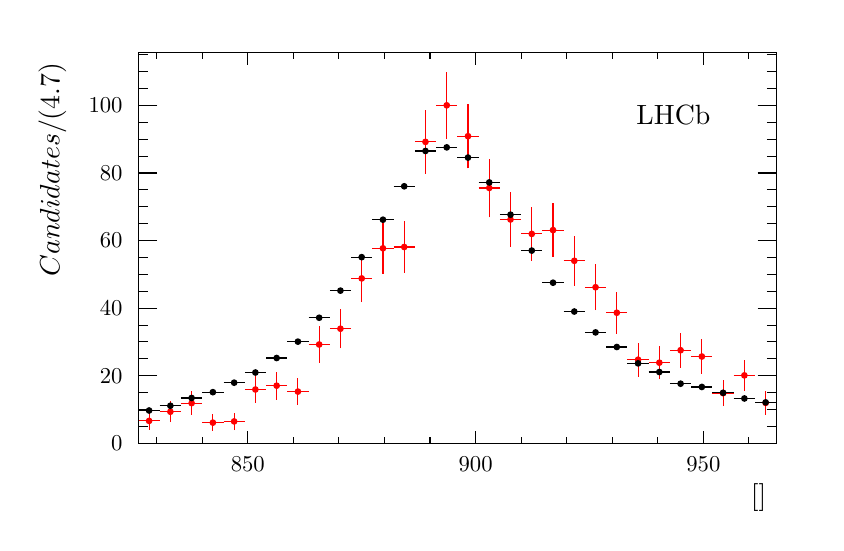
\begin{tikzpicture}
\pgfdeclareplotmark{cross} {
\pgfpathmoveto{\pgfpoint{-0.3\pgfplotmarksize}{\pgfplotmarksize}}
\pgfpathlineto{\pgfpoint{+0.3\pgfplotmarksize}{\pgfplotmarksize}}
\pgfpathlineto{\pgfpoint{+0.3\pgfplotmarksize}{0.3\pgfplotmarksize}}
\pgfpathlineto{\pgfpoint{+1\pgfplotmarksize}{0.3\pgfplotmarksize}}
\pgfpathlineto{\pgfpoint{+1\pgfplotmarksize}{-0.3\pgfplotmarksize}}
\pgfpathlineto{\pgfpoint{+0.3\pgfplotmarksize}{-0.3\pgfplotmarksize}}
\pgfpathlineto{\pgfpoint{+0.3\pgfplotmarksize}{-1.\pgfplotmarksize}}
\pgfpathlineto{\pgfpoint{-0.3\pgfplotmarksize}{-1.\pgfplotmarksize}}
\pgfpathlineto{\pgfpoint{-0.3\pgfplotmarksize}{-0.3\pgfplotmarksize}}
\pgfpathlineto{\pgfpoint{-1.\pgfplotmarksize}{-0.3\pgfplotmarksize}}
\pgfpathlineto{\pgfpoint{-1.\pgfplotmarksize}{0.3\pgfplotmarksize}}
\pgfpathlineto{\pgfpoint{-0.3\pgfplotmarksize}{0.3\pgfplotmarksize}}
\pgfpathclose
\pgfusepathqstroke
}
\pgfdeclareplotmark{cross*} {
\pgfpathmoveto{\pgfpoint{-0.3\pgfplotmarksize}{\pgfplotmarksize}}
\pgfpathlineto{\pgfpoint{+0.3\pgfplotmarksize}{\pgfplotmarksize}}
\pgfpathlineto{\pgfpoint{+0.3\pgfplotmarksize}{0.3\pgfplotmarksize}}
\pgfpathlineto{\pgfpoint{+1\pgfplotmarksize}{0.3\pgfplotmarksize}}
\pgfpathlineto{\pgfpoint{+1\pgfplotmarksize}{-0.3\pgfplotmarksize}}
\pgfpathlineto{\pgfpoint{+0.3\pgfplotmarksize}{-0.3\pgfplotmarksize}}
\pgfpathlineto{\pgfpoint{+0.3\pgfplotmarksize}{-1.\pgfplotmarksize}}
\pgfpathlineto{\pgfpoint{-0.3\pgfplotmarksize}{-1.\pgfplotmarksize}}
\pgfpathlineto{\pgfpoint{-0.3\pgfplotmarksize}{-0.3\pgfplotmarksize}}
\pgfpathlineto{\pgfpoint{-1.\pgfplotmarksize}{-0.3\pgfplotmarksize}}
\pgfpathlineto{\pgfpoint{-1.\pgfplotmarksize}{0.3\pgfplotmarksize}}
\pgfpathlineto{\pgfpoint{-0.3\pgfplotmarksize}{0.3\pgfplotmarksize}}
\pgfpathclose
\pgfusepathqfillstroke
}
\pgfdeclareplotmark{newstar} {
\pgfpathmoveto{\pgfqpoint{0pt}{\pgfplotmarksize}}
\pgfpathlineto{\pgfqpointpolar{44}{0.5\pgfplotmarksize}}
\pgfpathlineto{\pgfqpointpolar{18}{\pgfplotmarksize}}
\pgfpathlineto{\pgfqpointpolar{-20}{0.5\pgfplotmarksize}}
\pgfpathlineto{\pgfqpointpolar{-54}{\pgfplotmarksize}}
\pgfpathlineto{\pgfqpointpolar{-90}{0.5\pgfplotmarksize}}
\pgfpathlineto{\pgfqpointpolar{234}{\pgfplotmarksize}}
\pgfpathlineto{\pgfqpointpolar{198}{0.5\pgfplotmarksize}}
\pgfpathlineto{\pgfqpointpolar{162}{\pgfplotmarksize}}
\pgfpathlineto{\pgfqpointpolar{134}{0.5\pgfplotmarksize}}
\pgfpathclose
\pgfusepathqstroke
}
\pgfdeclareplotmark{newstar*} {
\pgfpathmoveto{\pgfqpoint{0pt}{\pgfplotmarksize}}
\pgfpathlineto{\pgfqpointpolar{44}{0.5\pgfplotmarksize}}
\pgfpathlineto{\pgfqpointpolar{18}{\pgfplotmarksize}}
\pgfpathlineto{\pgfqpointpolar{-20}{0.5\pgfplotmarksize}}
\pgfpathlineto{\pgfqpointpolar{-54}{\pgfplotmarksize}}
\pgfpathlineto{\pgfqpointpolar{-90}{0.5\pgfplotmarksize}}
\pgfpathlineto{\pgfqpointpolar{234}{\pgfplotmarksize}}
\pgfpathlineto{\pgfqpointpolar{198}{0.5\pgfplotmarksize}}
\pgfpathlineto{\pgfqpointpolar{162}{\pgfplotmarksize}}
\pgfpathlineto{\pgfqpointpolar{134}{0.5\pgfplotmarksize}}
\pgfpathclose
\pgfusepathqfillstroke
}
\definecolor{c}{rgb}{1,1,1};
\draw [color=c, fill=c] (0,0) rectangle (10,6.27517);
\draw [color=c, fill=c] (1.4,1.00403) rectangle (9.5,5.96141);
\definecolor{c}{rgb}{0,0,0};
\draw [c] (1.4,1.00403) -- (1.4,5.96141) -- (9.5,5.96141) -- (9.5,1.00403) -- (1.4,1.00403);
\definecolor{c}{rgb}{1,1,1};
\draw [color=c, fill=c] (1.4,1.00403) rectangle (9.5,5.96141);
\definecolor{c}{rgb}{0,0,0};
\draw [c] (1.4,1.00403) -- (1.4,5.96141) -- (9.5,5.96141) -- (9.5,1.00403) -- (1.4,1.00403);
\definecolor{c}{rgb}{1,0,0};
\draw [c,line width=0.4] (1.535,1.17784) -- (1.535,1.28827);
\draw [c,line width=0.4] (1.535,1.28827) -- (1.535,1.39869);
\draw [c,line width=0.4] (1.4,1.28827) -- (1.535,1.28827);
\draw [c,line width=0.4] (1.535,1.28827) -- (1.67,1.28827);
\foreach \P in {(1.535,1.28827)}{\draw[mark options={color=c,fill=c},mark size=2.402402pt,mark=*,mark size=1pt] plot coordinates {\P};}
\draw [c,line width=0.4] (1.805,1.27348) -- (1.805,1.40456);
\draw [c,line width=0.4] (1.805,1.40456) -- (1.805,1.53565);
\draw [c,line width=0.4] (1.67,1.40456) -- (1.805,1.40456);
\draw [c,line width=0.4] (1.805,1.40456) -- (1.94,1.40456);
\foreach \P in {(1.805,1.40456)}{\draw[mark options={color=c,fill=c},mark size=2.402402pt,mark=*,mark size=1pt] plot coordinates {\P};}
\draw [c,line width=0.4] (2.075,1.36594) -- (2.075,1.51382);
\draw [c,line width=0.4] (2.075,1.51382) -- (2.075,1.6617);
\draw [c,line width=0.4] (1.94,1.51382) -- (2.075,1.51382);
\draw [c,line width=0.4] (2.075,1.51382) -- (2.21,1.51382);
\foreach \P in {(2.075,1.51382)}{\draw[mark options={color=c,fill=c},mark size=2.402402pt,mark=*,mark size=1pt] plot coordinates {\P};}
\draw [c,line width=0.4] (2.345,1.16002) -- (2.345,1.26604);
\draw [c,line width=0.4] (2.345,1.26604) -- (2.345,1.37205);
\draw [c,line width=0.4] (2.21,1.26604) -- (2.345,1.26604);
\draw [c,line width=0.4] (2.345,1.26604) -- (2.48,1.26604);
\foreach \P in {(2.345,1.26604)}{\draw[mark options={color=c,fill=c},mark size=2.402402pt,mark=*,mark size=1pt] plot coordinates {\P};}
\draw [c,line width=0.4] (2.615,1.17259) -- (2.615,1.28174);
\draw [c,line width=0.4] (2.615,1.28174) -- (2.615,1.39089);
\draw [c,line width=0.4] (2.48,1.28174) -- (2.615,1.28174);
\draw [c,line width=0.4] (2.615,1.28174) -- (2.75,1.28174);
\foreach \P in {(2.615,1.28174)}{\draw[mark options={color=c,fill=c},mark size=2.402402pt,mark=*,mark size=1pt] plot coordinates {\P};}
\draw [c,line width=0.4] (2.885,1.51579) -- (2.885,1.68695);
\draw [c,line width=0.4] (2.885,1.68695) -- (2.885,1.85811);
\draw [c,line width=0.4] (2.75,1.68695) -- (2.885,1.68695);
\draw [c,line width=0.4] (2.885,1.68695) -- (3.02,1.68695);
\foreach \P in {(2.885,1.68695)}{\draw[mark options={color=c,fill=c},mark size=2.402402pt,mark=*,mark size=1pt] plot coordinates {\P};}
\draw [c,line width=0.4] (3.155,1.55856) -- (3.155,1.73572);
\draw [c,line width=0.4] (3.155,1.73572) -- (3.155,1.91289);
\draw [c,line width=0.4] (3.02,1.73572) -- (3.155,1.73572);
\draw [c,line width=0.4] (3.155,1.73572) -- (3.29,1.73572);
\foreach \P in {(3.155,1.73572)}{\draw[mark options={color=c,fill=c},mark size=2.402402pt,mark=*,mark size=1pt] plot coordinates {\P};}
\draw [c,line width=0.4] (3.425,1.49251) -- (3.425,1.6603);
\draw [c,line width=0.4] (3.425,1.6603) -- (3.425,1.82808);
\draw [c,line width=0.4] (3.29,1.6603) -- (3.425,1.6603);
\draw [c,line width=0.4] (3.425,1.6603) -- (3.56,1.6603);
\foreach \P in {(3.425,1.6603)}{\draw[mark options={color=c,fill=c},mark size=2.402402pt,mark=*,mark size=1pt] plot coordinates {\P};}
\draw [c,line width=0.4] (3.695,2.02663) -- (3.695,2.25862);
\draw [c,line width=0.4] (3.695,2.25862) -- (3.695,2.49061);
\draw [c,line width=0.4] (3.56,2.25862) -- (3.695,2.25862);
\draw [c,line width=0.4] (3.695,2.25862) -- (3.83,2.25862);
\foreach \P in {(3.695,2.25862)}{\draw[mark options={color=c,fill=c},mark size=2.402402pt,mark=*,mark size=1pt] plot coordinates {\P};}
\draw [c,line width=0.4] (3.965,2.209) -- (3.965,2.45881);
\draw [c,line width=0.4] (3.965,2.45881) -- (3.965,2.70862);
\draw [c,line width=0.4] (3.83,2.45881) -- (3.965,2.45881);
\draw [c,line width=0.4] (3.965,2.45881) -- (4.1,2.45881);
\foreach \P in {(3.965,2.45881)}{\draw[mark options={color=c,fill=c},mark size=2.402402pt,mark=*,mark size=1pt] plot coordinates {\P};}
\draw [c,line width=0.4] (4.235,2.79809) -- (4.235,3.09778);
\draw [c,line width=0.4] (4.235,3.09778) -- (4.235,3.39748);
\draw [c,line width=0.4] (4.1,3.09778) -- (4.235,3.09778);
\draw [c,line width=0.4] (4.235,3.09778) -- (4.37,3.09778);
\foreach \P in {(4.235,3.09778)}{\draw[mark options={color=c,fill=c},mark size=2.402402pt,mark=*,mark size=1pt] plot coordinates {\P};}
\draw [c,line width=0.4] (4.505,3.1545) -- (4.505,3.48044);
\draw [c,line width=0.4] (4.505,3.48044) -- (4.505,3.80637);
\draw [c,line width=0.4] (4.37,3.48044) -- (4.505,3.48044);
\draw [c,line width=0.4] (4.505,3.48044) -- (4.64,3.48044);
\foreach \P in {(4.505,3.48044)}{\draw[mark options={color=c,fill=c},mark size=2.402402pt,mark=*,mark size=1pt] plot coordinates {\P};}
\draw [c,line width=0.4] (4.775,3.16967) -- (4.775,3.49667);
\draw [c,line width=0.4] (4.775,3.49667) -- (4.775,3.82366);
\draw [c,line width=0.4] (4.64,3.49667) -- (4.775,3.49667);
\draw [c,line width=0.4] (4.775,3.49667) -- (4.91,3.49667);
\foreach \P in {(4.775,3.49667)}{\draw[mark options={color=c,fill=c},mark size=2.402402pt,mark=*,mark size=1pt] plot coordinates {\P};}
\draw [c,line width=0.4] (5.045,4.42665) -- (5.045,4.83187);
\draw [c,line width=0.4] (5.045,4.83187) -- (5.045,5.23709);
\draw [c,line width=0.4] (4.91,4.83187) -- (5.045,4.83187);
\draw [c,line width=0.4] (5.045,4.83187) -- (5.18,4.83187);
\foreach \P in {(5.045,4.83187)}{\draw[mark options={color=c,fill=c},mark size=2.402402pt,mark=*,mark size=1pt] plot coordinates {\P};}
\draw [c,line width=0.4] (5.315,4.86715) -- (5.315,5.29625);
\draw [c,line width=0.4] (5.315,5.29625) -- (5.315,5.72534);
\draw [c,line width=0.4] (5.18,5.29625) -- (5.315,5.29625);
\draw [c,line width=0.4] (5.315,5.29625) -- (5.45,5.29625);
\foreach \P in {(5.315,5.29625)}{\draw[mark options={color=c,fill=c},mark size=2.402402pt,mark=*,mark size=1pt] plot coordinates {\P};}
\draw [c,line width=0.4] (5.585,4.4952) -- (5.585,4.90423);
\draw [c,line width=0.4] (5.585,4.90423) -- (5.585,5.31327);
\draw [c,line width=0.4] (5.45,4.90423) -- (5.585,4.90423);
\draw [c,line width=0.4] (5.585,4.90423) -- (5.72,4.90423);
\foreach \P in {(5.585,4.90423)}{\draw[mark options={color=c,fill=c},mark size=2.402402pt,mark=*,mark size=1pt] plot coordinates {\P};}
\draw [c,line width=0.4] (5.855,3.87371) -- (5.855,4.24667);
\draw [c,line width=0.4] (5.855,4.24667) -- (5.855,4.61964);
\draw [c,line width=0.4] (5.72,4.24667) -- (5.855,4.24667);
\draw [c,line width=0.4] (5.855,4.24667) -- (5.99,4.24667);
\foreach \P in {(5.855,4.24667)}{\draw[mark options={color=c,fill=c},mark size=2.402402pt,mark=*,mark size=1pt] plot coordinates {\P};}
\draw [c,line width=0.4] (6.125,3.49716) -- (6.125,3.84635);
\draw [c,line width=0.4] (6.125,3.84635) -- (6.125,4.19553);
\draw [c,line width=0.4] (5.99,3.84635) -- (6.125,3.84635);
\draw [c,line width=0.4] (6.125,3.84635) -- (6.26,3.84635);
\foreach \P in {(6.125,3.84635)}{\draw[mark options={color=c,fill=c},mark size=2.402402pt,mark=*,mark size=1pt] plot coordinates {\P};}
\draw [c,line width=0.4] (6.395,3.32518) -- (6.395,3.66291);
\draw [c,line width=0.4] (6.395,3.66291) -- (6.395,4.00064);
\draw [c,line width=0.4] (6.26,3.66291) -- (6.395,3.66291);
\draw [c,line width=0.4] (6.395,3.66291) -- (6.53,3.66291);
\foreach \P in {(6.395,3.66291)}{\draw[mark options={color=c,fill=c},mark size=2.402402pt,mark=*,mark size=1pt] plot coordinates {\P};}
\draw [c,line width=0.4] (6.665,3.37055) -- (6.665,3.71134);
\draw [c,line width=0.4] (6.665,3.71134) -- (6.665,4.05213);
\draw [c,line width=0.4] (6.53,3.71134) -- (6.665,3.71134);
\draw [c,line width=0.4] (6.665,3.71134) -- (6.8,3.71134);
\foreach \P in {(6.665,3.71134)}{\draw[mark options={color=c,fill=c},mark size=2.402402pt,mark=*,mark size=1pt] plot coordinates {\P};}
\draw [c,line width=0.4] (6.935,3.00614) -- (6.935,3.32143);
\draw [c,line width=0.4] (6.935,3.32143) -- (6.935,3.63673);
\draw [c,line width=0.4] (6.8,3.32143) -- (6.935,3.32143);
\draw [c,line width=0.4] (6.935,3.32143) -- (7.07,3.32143);
\foreach \P in {(6.935,3.32143)}{\draw[mark options={color=c,fill=c},mark size=2.402402pt,mark=*,mark size=1pt] plot coordinates {\P};}
\draw [c,line width=0.4] (7.205,2.69423) -- (7.205,2.9858);
\draw [c,line width=0.4] (7.205,2.9858) -- (7.205,3.27737);
\draw [c,line width=0.4] (7.07,2.9858) -- (7.205,2.9858);
\draw [c,line width=0.4] (7.205,2.9858) -- (7.34,2.9858);
\foreach \P in {(7.205,2.9858)}{\draw[mark options={color=c,fill=c},mark size=2.402402pt,mark=*,mark size=1pt] plot coordinates {\P};}
\draw [c,line width=0.4] (7.475,2.39511) -- (7.475,2.66178);
\draw [c,line width=0.4] (7.475,2.66178) -- (7.475,2.92845);
\draw [c,line width=0.4] (7.34,2.66178) -- (7.475,2.66178);
\draw [c,line width=0.4] (7.475,2.66178) -- (7.61,2.66178);
\foreach \P in {(7.475,2.66178)}{\draw[mark options={color=c,fill=c},mark size=2.402402pt,mark=*,mark size=1pt] plot coordinates {\P};}
\draw [c,line width=0.4] (7.745,1.85202) -- (7.745,2.0654);
\draw [c,line width=0.4] (7.745,2.0654) -- (7.745,2.27878);
\draw [c,line width=0.4] (7.61,2.0654) -- (7.745,2.0654);
\draw [c,line width=0.4] (7.745,2.0654) -- (7.88,2.0654);
\foreach \P in {(7.745,2.0654)}{\draw[mark options={color=c,fill=c},mark size=2.402402pt,mark=*,mark size=1pt] plot coordinates {\P};}
\draw [c,line width=0.4] (8.015,1.81816) -- (8.015,2.02772);
\draw [c,line width=0.4] (8.015,2.02772) -- (8.015,2.23728);
\draw [c,line width=0.4] (7.88,2.02772) -- (8.015,2.02772);
\draw [c,line width=0.4] (8.015,2.02772) -- (8.15,2.02772);
\foreach \P in {(8.015,2.02772)}{\draw[mark options={color=c,fill=c},mark size=2.402402pt,mark=*,mark size=1pt] plot coordinates {\P};}
\draw [c,line width=0.4] (8.285,1.96043) -- (8.285,2.18556);
\draw [c,line width=0.4] (8.285,2.18556) -- (8.285,2.4107);
\draw [c,line width=0.4] (8.15,2.18556) -- (8.285,2.18556);
\draw [c,line width=0.4] (8.285,2.18556) -- (8.42,2.18556);
\foreach \P in {(8.285,2.18556)}{\draw[mark options={color=c,fill=c},mark size=2.402402pt,mark=*,mark size=1pt] plot coordinates {\P};}
\draw [c,line width=0.4] (8.555,1.88822) -- (8.555,2.1056);
\draw [c,line width=0.4] (8.555,2.1056) -- (8.555,2.32299);
\draw [c,line width=0.4] (8.42,2.1056) -- (8.555,2.1056);
\draw [c,line width=0.4] (8.555,2.1056) -- (8.69,2.1056);
\foreach \P in {(8.555,2.1056)}{\draw[mark options={color=c,fill=c},mark size=2.402402pt,mark=*,mark size=1pt] plot coordinates {\P};}
\draw [c,line width=0.4] (8.825,1.47523) -- (8.825,1.64046);
\draw [c,line width=0.4] (8.825,1.64046) -- (8.825,1.80569);
\draw [c,line width=0.4] (8.69,1.64046) -- (8.825,1.64046);
\draw [c,line width=0.4] (8.825,1.64046) -- (8.96,1.64046);
\foreach \P in {(8.825,1.64046)}{\draw[mark options={color=c,fill=c},mark size=2.402402pt,mark=*,mark size=1pt] plot coordinates {\P};}
\draw [c,line width=0.4] (9.095,1.67404) -- (9.095,1.86638);
\draw [c,line width=0.4] (9.095,1.86638) -- (9.095,2.05871);
\draw [c,line width=0.4] (8.96,1.86638) -- (9.095,1.86638);
\draw [c,line width=0.4] (9.095,1.86638) -- (9.23,1.86638);
\foreach \P in {(9.095,1.86638)}{\draw[mark options={color=c,fill=c},mark size=2.402402pt,mark=*,mark size=1pt] plot coordinates {\P};}
\draw [c,line width=0.4] (9.365,1.36845) -- (9.365,1.51676);
\draw [c,line width=0.4] (9.365,1.51676) -- (9.365,1.66507);
\draw [c,line width=0.4] (9.23,1.51676) -- (9.365,1.51676);
\draw [c,line width=0.4] (9.365,1.51676) -- (9.5,1.51676);
\foreach \P in {(9.365,1.51676)}{\draw[mark options={color=c,fill=c},mark size=2.402402pt,mark=*,mark size=1pt] plot coordinates {\P};}
\definecolor{c}{rgb}{0,0,0};
\draw [c,line width=0.4] (1.4,1.00403) -- (9.5,1.00403);
\draw [anchor= east] (9.5,0.317272) node[scale=1.00614, rotate=0]{$\mkpi [\mevcc]$};
\draw [c,line width=0.4] (2.78857,1.15651) -- (2.78857,1.00403);
\draw [c,line width=0.4] (3.36714,1.08027) -- (3.36714,1.00403);
\draw [c,line width=0.4] (3.94571,1.08027) -- (3.94571,1.00403);
\draw [c,line width=0.4] (4.52429,1.08027) -- (4.52429,1.00403);
\draw [c,line width=0.4] (5.10286,1.08027) -- (5.10286,1.00403);
\draw [c,line width=0.4] (5.68143,1.15651) -- (5.68143,1.00403);
\draw [c,line width=0.4] (6.26,1.08027) -- (6.26,1.00403);
\draw [c,line width=0.4] (6.83857,1.08027) -- (6.83857,1.00403);
\draw [c,line width=0.4] (7.41714,1.08027) -- (7.41714,1.00403);
\draw [c,line width=0.4] (7.99571,1.08027) -- (7.99571,1.00403);
\draw [c,line width=0.4] (8.57429,1.15651) -- (8.57429,1.00403);
\draw [c,line width=0.4] (2.78857,1.15651) -- (2.78857,1.00403);
\draw [c,line width=0.4] (2.21,1.08027) -- (2.21,1.00403);
\draw [c,line width=0.4] (1.63143,1.08027) -- (1.63143,1.00403);
\draw [c,line width=0.4] (8.57429,1.15651) -- (8.57429,1.00403);
\draw [c,line width=0.4] (9.15286,1.08027) -- (9.15286,1.00403);
\draw [anchor=base] (2.78857,0.640067) node[scale=0.819821, rotate=0]{850};
\draw [anchor=base] (5.68143,0.640067) node[scale=0.819821, rotate=0]{900};
\draw [anchor=base] (8.57429,0.640067) node[scale=0.819821, rotate=0]{950};
\draw [c,line width=0.4] (1.4,5.96141) -- (9.5,5.96141);
\draw [c,line width=0.4] (2.78857,5.80892) -- (2.78857,5.96141);
\draw [c,line width=0.4] (3.36714,5.88517) -- (3.36714,5.96141);
\draw [c,line width=0.4] (3.94571,5.88517) -- (3.94571,5.96141);
\draw [c,line width=0.4] (4.52429,5.88517) -- (4.52429,5.96141);
\draw [c,line width=0.4] (5.10286,5.88517) -- (5.10286,5.96141);
\draw [c,line width=0.4] (5.68143,5.80892) -- (5.68143,5.96141);
\draw [c,line width=0.4] (6.26,5.88517) -- (6.26,5.96141);
\draw [c,line width=0.4] (6.83857,5.88517) -- (6.83857,5.96141);
\draw [c,line width=0.4] (7.41714,5.88517) -- (7.41714,5.96141);
\draw [c,line width=0.4] (7.99571,5.88517) -- (7.99571,5.96141);
\draw [c,line width=0.4] (8.57429,5.80892) -- (8.57429,5.96141);
\draw [c,line width=0.4] (2.78857,5.80892) -- (2.78857,5.96141);
\draw [c,line width=0.4] (2.21,5.88517) -- (2.21,5.96141);
\draw [c,line width=0.4] (1.63143,5.88517) -- (1.63143,5.96141);
\draw [c,line width=0.4] (8.57429,5.80892) -- (8.57429,5.96141);
\draw [c,line width=0.4] (9.15286,5.88517) -- (9.15286,5.96141);
\draw [c,line width=0.4] (1.4,1.00403) -- (1.4,5.96141);
\draw [anchor= east] (0.3056,5.96141) node[scale=1.00614, rotate=90]{$\text{Candidates} / (4.7 \mevcc)$};
\draw [c,line width=0.4] (1.637,1.00403) -- (1.4,1.00403);
\draw [c,line width=0.4] (1.5185,1.21851) -- (1.4,1.21851);
\draw [c,line width=0.4] (1.5185,1.433) -- (1.4,1.433);
\draw [c,line width=0.4] (1.5185,1.64749) -- (1.4,1.64749);
\draw [c,line width=0.4] (1.637,1.86198) -- (1.4,1.86198);
\draw [c,line width=0.4] (1.5185,2.07647) -- (1.4,2.07647);
\draw [c,line width=0.4] (1.5185,2.29095) -- (1.4,2.29095);
\draw [c,line width=0.4] (1.5185,2.50544) -- (1.4,2.50544);
\draw [c,line width=0.4] (1.637,2.71993) -- (1.4,2.71993);
\draw [c,line width=0.4] (1.5185,2.93442) -- (1.4,2.93442);
\draw [c,line width=0.4] (1.5185,3.1489) -- (1.4,3.1489);
\draw [c,line width=0.4] (1.5185,3.36339) -- (1.4,3.36339);
\draw [c,line width=0.4] (1.637,3.57788) -- (1.4,3.57788);
\draw [c,line width=0.4] (1.5185,3.79237) -- (1.4,3.79237);
\draw [c,line width=0.4] (1.5185,4.00686) -- (1.4,4.00686);
\draw [c,line width=0.4] (1.5185,4.22134) -- (1.4,4.22134);
\draw [c,line width=0.4] (1.637,4.43583) -- (1.4,4.43583);
\draw [c,line width=0.4] (1.5185,4.65032) -- (1.4,4.65032);
\draw [c,line width=0.4] (1.5185,4.86481) -- (1.4,4.86481);
\draw [c,line width=0.4] (1.5185,5.07929) -- (1.4,5.07929);
\draw [c,line width=0.4] (1.637,5.29378) -- (1.4,5.29378);
\draw [c,line width=0.4] (1.637,5.29378) -- (1.4,5.29378);
\draw [c,line width=0.4] (1.5185,5.50827) -- (1.4,5.50827);
\draw [c,line width=0.4] (1.5185,5.72276) -- (1.4,5.72276);
\draw [c,line width=0.4] (1.5185,5.93724) -- (1.4,5.93724);
\draw [anchor= east] (1.3,1.00403) node[scale=0.819821, rotate=0]{0};
\draw [anchor= east] (1.3,1.86198) node[scale=0.819821, rotate=0]{20};
\draw [anchor= east] (1.3,2.71993) node[scale=0.819821, rotate=0]{40};
\draw [anchor= east] (1.3,3.57788) node[scale=0.819821, rotate=0]{60};
\draw [anchor= east] (1.3,4.43583) node[scale=0.819821, rotate=0]{80};
\draw [anchor= east] (1.3,5.29378) node[scale=0.819821, rotate=0]{100};
\draw [c,line width=0.4] (9.5,1.00403) -- (9.5,5.96141);
\draw [c,line width=0.4] (9.263,1.00403) -- (9.5,1.00403);
\draw [c,line width=0.4] (9.3815,1.21851) -- (9.5,1.21851);
\draw [c,line width=0.4] (9.3815,1.433) -- (9.5,1.433);
\draw [c,line width=0.4] (9.3815,1.64749) -- (9.5,1.64749);
\draw [c,line width=0.4] (9.263,1.86198) -- (9.5,1.86198);
\draw [c,line width=0.4] (9.3815,2.07647) -- (9.5,2.07647);
\draw [c,line width=0.4] (9.3815,2.29095) -- (9.5,2.29095);
\draw [c,line width=0.4] (9.3815,2.50544) -- (9.5,2.50544);
\draw [c,line width=0.4] (9.263,2.71993) -- (9.5,2.71993);
\draw [c,line width=0.4] (9.3815,2.93442) -- (9.5,2.93442);
\draw [c,line width=0.4] (9.3815,3.1489) -- (9.5,3.1489);
\draw [c,line width=0.4] (9.3815,3.36339) -- (9.5,3.36339);
\draw [c,line width=0.4] (9.263,3.57788) -- (9.5,3.57788);
\draw [c,line width=0.4] (9.3815,3.79237) -- (9.5,3.79237);
\draw [c,line width=0.4] (9.3815,4.00686) -- (9.5,4.00686);
\draw [c,line width=0.4] (9.3815,4.22134) -- (9.5,4.22134);
\draw [c,line width=0.4] (9.263,4.43583) -- (9.5,4.43583);
\draw [c,line width=0.4] (9.3815,4.65032) -- (9.5,4.65032);
\draw [c,line width=0.4] (9.3815,4.86481) -- (9.5,4.86481);
\draw [c,line width=0.4] (9.3815,5.07929) -- (9.5,5.07929);
\draw [c,line width=0.4] (9.263,5.29378) -- (9.5,5.29378);
\draw [c,line width=0.4] (9.263,5.29378) -- (9.5,5.29378);
\draw [c,line width=0.4] (9.3815,5.50827) -- (9.5,5.50827);
\draw [c,line width=0.4] (9.3815,5.72276) -- (9.5,5.72276);
\draw [c,line width=0.4] (9.3815,5.93724) -- (9.5,5.93724);
\draw [c,line width=0.4] (1.535,1.41014) -- (1.535,1.42026);
\draw [c,line width=0.4] (1.535,1.42026) -- (1.535,1.43038);
\draw [c,line width=0.4] (1.4,1.42026) -- (1.535,1.42026);
\draw [c,line width=0.4] (1.535,1.42026) -- (1.67,1.42026);
\foreach \P in {(1.535,1.42026)}{\draw[mark options={color=c,fill=c},mark size=2.402402pt,mark=*,mark size=1pt] plot coordinates {\P};}
\draw [c,line width=0.4] (1.805,1.46974) -- (1.805,1.48057);
\draw [c,line width=0.4] (1.805,1.48057) -- (1.805,1.4914);
\draw [c,line width=0.4] (1.67,1.48057) -- (1.805,1.48057);
\draw [c,line width=0.4] (1.805,1.48057) -- (1.94,1.48057);
\foreach \P in {(1.805,1.48057)}{\draw[mark options={color=c,fill=c},mark size=2.402402pt,mark=*,mark size=1pt] plot coordinates {\P};}
\draw [c,line width=0.4] (2.075,1.56752) -- (2.075,1.57942);
\draw [c,line width=0.4] (2.075,1.57942) -- (2.075,1.59133);
\draw [c,line width=0.4] (1.94,1.57942) -- (2.075,1.57942);
\draw [c,line width=0.4] (2.075,1.57942) -- (2.21,1.57942);
\foreach \P in {(2.075,1.57942)}{\draw[mark options={color=c,fill=c},mark size=2.402402pt,mark=*,mark size=1pt] plot coordinates {\P};}
\draw [c,line width=0.4] (2.345,1.64049) -- (2.345,1.65313);
\draw [c,line width=0.4] (2.345,1.65313) -- (2.345,1.66577);
\draw [c,line width=0.4] (2.21,1.65313) -- (2.345,1.65313);
\draw [c,line width=0.4] (2.345,1.65313) -- (2.48,1.65313);
\foreach \P in {(2.345,1.65313)}{\draw[mark options={color=c,fill=c},mark size=2.402402pt,mark=*,mark size=1pt] plot coordinates {\P};}
\draw [c,line width=0.4] (2.615,1.75977) -- (2.615,1.77354);
\draw [c,line width=0.4] (2.615,1.77354) -- (2.615,1.7873);
\draw [c,line width=0.4] (2.48,1.77354) -- (2.615,1.77354);
\draw [c,line width=0.4] (2.615,1.77354) -- (2.75,1.77354);
\foreach \P in {(2.615,1.77354)}{\draw[mark options={color=c,fill=c},mark size=2.402402pt,mark=*,mark size=1pt] plot coordinates {\P};}
\draw [c,line width=0.4] (2.885,1.88793) -- (2.885,1.9028);
\draw [c,line width=0.4] (2.885,1.9028) -- (2.885,1.91768);
\draw [c,line width=0.4] (2.75,1.9028) -- (2.885,1.9028);
\draw [c,line width=0.4] (2.885,1.9028) -- (3.02,1.9028);
\foreach \P in {(2.885,1.9028)}{\draw[mark options={color=c,fill=c},mark size=2.402402pt,mark=*,mark size=1pt] plot coordinates {\P};}
\draw [c,line width=0.4] (3.155,2.07054) -- (3.155,2.08687);
\draw [c,line width=0.4] (3.155,2.08687) -- (3.155,2.1032);
\draw [c,line width=0.4] (3.02,2.08687) -- (3.155,2.08687);
\draw [c,line width=0.4] (3.155,2.08687) -- (3.29,2.08687);
\foreach \P in {(3.155,2.08687)}{\draw[mark options={color=c,fill=c},mark size=2.402402pt,mark=*,mark size=1pt] plot coordinates {\P};}
\draw [c,line width=0.4] (3.425,2.2771) -- (3.425,2.29493);
\draw [c,line width=0.4] (3.425,2.29493) -- (3.425,2.31276);
\draw [c,line width=0.4] (3.29,2.29493) -- (3.425,2.29493);
\draw [c,line width=0.4] (3.425,2.29493) -- (3.56,2.29493);
\foreach \P in {(3.425,2.29493)}{\draw[mark options={color=c,fill=c},mark size=2.402402pt,mark=*,mark size=1pt] plot coordinates {\P};}
\draw [c,line width=0.4] (3.695,2.57837) -- (3.695,2.59818);
\draw [c,line width=0.4] (3.695,2.59818) -- (3.695,2.618);
\draw [c,line width=0.4] (3.56,2.59818) -- (3.695,2.59818);
\draw [c,line width=0.4] (3.695,2.59818) -- (3.83,2.59818);
\foreach \P in {(3.695,2.59818)}{\draw[mark options={color=c,fill=c},mark size=2.402402pt,mark=*,mark size=1pt] plot coordinates {\P};}
\draw [c,line width=0.4] (3.965,2.92076) -- (3.965,2.94261);
\draw [c,line width=0.4] (3.965,2.94261) -- (3.965,2.96446);
\draw [c,line width=0.4] (3.83,2.94261) -- (3.965,2.94261);
\draw [c,line width=0.4] (3.965,2.94261) -- (4.1,2.94261);
\foreach \P in {(3.965,2.94261)}{\draw[mark options={color=c,fill=c},mark size=2.402402pt,mark=*,mark size=1pt] plot coordinates {\P};}
\draw [c,line width=0.4] (4.235,3.34382) -- (4.235,3.36795);
\draw [c,line width=0.4] (4.235,3.36795) -- (4.235,3.39208);
\draw [c,line width=0.4] (4.1,3.36795) -- (4.235,3.36795);
\draw [c,line width=0.4] (4.235,3.36795) -- (4.37,3.36795);
\foreach \P in {(4.235,3.36795)}{\draw[mark options={color=c,fill=c},mark size=2.402402pt,mark=*,mark size=1pt] plot coordinates {\P};}
\draw [c,line width=0.4] (4.505,3.81695) -- (4.505,3.84339);
\draw [c,line width=0.4] (4.505,3.84339) -- (4.505,3.86984);
\draw [c,line width=0.4] (4.37,3.84339) -- (4.505,3.84339);
\draw [c,line width=0.4] (4.505,3.84339) -- (4.64,3.84339);
\foreach \P in {(4.505,3.84339)}{\draw[mark options={color=c,fill=c},mark size=2.402402pt,mark=*,mark size=1pt] plot coordinates {\P};}
\draw [c,line width=0.4] (4.775,4.23942) -- (4.775,4.26777);
\draw [c,line width=0.4] (4.775,4.26777) -- (4.775,4.29612);
\draw [c,line width=0.4] (4.64,4.26777) -- (4.775,4.26777);
\draw [c,line width=0.4] (4.775,4.26777) -- (4.91,4.26777);
\foreach \P in {(4.775,4.26777)}{\draw[mark options={color=c,fill=c},mark size=2.402402pt,mark=*,mark size=1pt] plot coordinates {\P};}
\draw [c,line width=0.4] (5.045,4.68612) -- (5.045,4.71636);
\draw [c,line width=0.4] (5.045,4.71636) -- (5.045,4.7466);
\draw [c,line width=0.4] (4.91,4.71636) -- (5.045,4.71636);
\draw [c,line width=0.4] (5.045,4.71636) -- (5.18,4.71636);
\foreach \P in {(5.045,4.71636)}{\draw[mark options={color=c,fill=c},mark size=2.402402pt,mark=*,mark size=1pt] plot coordinates {\P};}
\draw [c,line width=0.4] (5.315,4.73167) -- (5.315,4.76209);
\draw [c,line width=0.4] (5.315,4.76209) -- (5.315,4.79251);
\draw [c,line width=0.4] (5.18,4.76209) -- (5.315,4.76209);
\draw [c,line width=0.4] (5.315,4.76209) -- (5.45,4.76209);
\foreach \P in {(5.315,4.76209)}{\draw[mark options={color=c,fill=c},mark size=2.402402pt,mark=*,mark size=1pt] plot coordinates {\P};}
\draw [c,line width=0.4] (5.585,4.60254) -- (5.585,4.63244);
\draw [c,line width=0.4] (5.585,4.63244) -- (5.585,4.66233);
\draw [c,line width=0.4] (5.45,4.63244) -- (5.585,4.63244);
\draw [c,line width=0.4] (5.585,4.63244) -- (5.72,4.63244);
\foreach \P in {(5.585,4.63244)}{\draw[mark options={color=c,fill=c},mark size=2.402402pt,mark=*,mark size=1pt] plot coordinates {\P};}
\draw [c,line width=0.4] (5.855,4.28818) -- (5.855,4.31675);
\draw [c,line width=0.4] (5.855,4.31675) -- (5.855,4.34531);
\draw [c,line width=0.4] (5.72,4.31675) -- (5.855,4.31675);
\draw [c,line width=0.4] (5.855,4.31675) -- (5.99,4.31675);
\foreach \P in {(5.855,4.31675)}{\draw[mark options={color=c,fill=c},mark size=2.402402pt,mark=*,mark size=1pt] plot coordinates {\P};}
\draw [c,line width=0.4] (6.125,3.88034) -- (6.125,3.90708);
\draw [c,line width=0.4] (6.125,3.90708) -- (6.125,3.93382);
\draw [c,line width=0.4] (5.99,3.90708) -- (6.125,3.90708);
\draw [c,line width=0.4] (6.125,3.90708) -- (6.26,3.90708);
\foreach \P in {(6.125,3.90708)}{\draw[mark options={color=c,fill=c},mark size=2.402402pt,mark=*,mark size=1pt] plot coordinates {\P};}
\draw [c,line width=0.4] (6.395,3.42666) -- (6.395,3.45121);
\draw [c,line width=0.4] (6.395,3.45121) -- (6.395,3.47576);
\draw [c,line width=0.4] (6.26,3.45121) -- (6.395,3.45121);
\draw [c,line width=0.4] (6.395,3.45121) -- (6.53,3.45121);
\foreach \P in {(6.395,3.45121)}{\draw[mark options={color=c,fill=c},mark size=2.402402pt,mark=*,mark size=1pt] plot coordinates {\P};}
\draw [c,line width=0.4] (6.665,3.02074) -- (6.665,3.04315);
\draw [c,line width=0.4] (6.665,3.04315) -- (6.665,3.06556);
\draw [c,line width=0.4] (6.53,3.04315) -- (6.665,3.04315);
\draw [c,line width=0.4] (6.665,3.04315) -- (6.8,3.04315);
\foreach \P in {(6.665,3.04315)}{\draw[mark options={color=c,fill=c},mark size=2.402402pt,mark=*,mark size=1pt] plot coordinates {\P};}
\draw [c,line width=0.4] (6.935,2.65694) -- (6.935,2.67724);
\draw [c,line width=0.4] (6.935,2.67724) -- (6.935,2.69754);
\draw [c,line width=0.4] (6.8,2.67724) -- (6.935,2.67724);
\draw [c,line width=0.4] (6.935,2.67724) -- (7.07,2.67724);
\foreach \P in {(6.935,2.67724)}{\draw[mark options={color=c,fill=c},mark size=2.402402pt,mark=*,mark size=1pt] plot coordinates {\P};}
\draw [c,line width=0.4] (7.205,2.39361) -- (7.205,2.41223);
\draw [c,line width=0.4] (7.205,2.41223) -- (7.205,2.43086);
\draw [c,line width=0.4] (7.07,2.41223) -- (7.205,2.41223);
\draw [c,line width=0.4] (7.205,2.41223) -- (7.34,2.41223);
\foreach \P in {(7.205,2.41223)}{\draw[mark options={color=c,fill=c},mark size=2.402402pt,mark=*,mark size=1pt] plot coordinates {\P};}
\draw [c,line width=0.4] (7.475,2.20922) -- (7.475,2.22657);
\draw [c,line width=0.4] (7.475,2.22657) -- (7.475,2.24392);
\draw [c,line width=0.4] (7.34,2.22657) -- (7.475,2.22657);
\draw [c,line width=0.4] (7.475,2.22657) -- (7.61,2.22657);
\foreach \P in {(7.475,2.22657)}{\draw[mark options={color=c,fill=c},mark size=2.402402pt,mark=*,mark size=1pt] plot coordinates {\P};}
\draw [c,line width=0.4] (7.745,2.00304) -- (7.745,2.01885);
\draw [c,line width=0.4] (7.745,2.01885) -- (7.745,2.03466);
\draw [c,line width=0.4] (7.61,2.01885) -- (7.745,2.01885);
\draw [c,line width=0.4] (7.745,2.01885) -- (7.88,2.01885);
\foreach \P in {(7.745,2.01885)}{\draw[mark options={color=c,fill=c},mark size=2.402402pt,mark=*,mark size=1pt] plot coordinates {\P};}
\draw [c,line width=0.4] (8.015,1.89412) -- (8.015,1.90905);
\draw [c,line width=0.4] (8.015,1.90905) -- (8.015,1.92398);
\draw [c,line width=0.4] (7.88,1.90905) -- (8.015,1.90905);
\draw [c,line width=0.4] (8.015,1.90905) -- (8.15,1.90905);
\foreach \P in {(8.015,1.90905)}{\draw[mark options={color=c,fill=c},mark size=2.402402pt,mark=*,mark size=1pt] plot coordinates {\P};}
\draw [c,line width=0.4] (8.285,1.74702) -- (8.285,1.76067);
\draw [c,line width=0.4] (8.285,1.76067) -- (8.285,1.77432);
\draw [c,line width=0.4] (8.15,1.76067) -- (8.285,1.76067);
\draw [c,line width=0.4] (8.285,1.76067) -- (8.42,1.76067);
\foreach \P in {(8.285,1.76067)}{\draw[mark options={color=c,fill=c},mark size=2.402402pt,mark=*,mark size=1pt] plot coordinates {\P};}
\draw [c,line width=0.4] (8.555,1.70609) -- (8.555,1.71936);
\draw [c,line width=0.4] (8.555,1.71936) -- (8.555,1.73263);
\draw [c,line width=0.4] (8.42,1.71936) -- (8.555,1.71936);
\draw [c,line width=0.4] (8.555,1.71936) -- (8.69,1.71936);
\foreach \P in {(8.555,1.71936)}{\draw[mark options={color=c,fill=c},mark size=2.402402pt,mark=*,mark size=1pt] plot coordinates {\P};}
\draw [c,line width=0.4] (8.825,1.63255) -- (8.825,1.64512);
\draw [c,line width=0.4] (8.825,1.64512) -- (8.825,1.65768);
\draw [c,line width=0.4] (8.69,1.64512) -- (8.825,1.64512);
\draw [c,line width=0.4] (8.825,1.64512) -- (8.96,1.64512);
\foreach \P in {(8.825,1.64512)}{\draw[mark options={color=c,fill=c},mark size=2.402402pt,mark=*,mark size=1pt] plot coordinates {\P};}
\draw [c,line width=0.4] (9.095,1.56134) -- (9.095,1.57318);
\draw [c,line width=0.4] (9.095,1.57318) -- (9.095,1.58502);
\draw [c,line width=0.4] (8.96,1.57318) -- (9.095,1.57318);
\draw [c,line width=0.4] (9.095,1.57318) -- (9.23,1.57318);
\foreach \P in {(9.095,1.57318)}{\draw[mark options={color=c,fill=c},mark size=2.402402pt,mark=*,mark size=1pt] plot coordinates {\P};}
\draw [c,line width=0.4] (9.365,1.51213) -- (9.365,1.52344);
\draw [c,line width=0.4] (9.365,1.52344) -- (9.365,1.53475);
\draw [c,line width=0.4] (9.23,1.52344) -- (9.365,1.52344);
\draw [c,line width=0.4] (9.365,1.52344) -- (9.5,1.52344);
\foreach \P in {(9.365,1.52344)}{\draw[mark options={color=c,fill=c},mark size=2.402402pt,mark=*,mark size=1pt] plot coordinates {\P};}
\draw [anchor= west] (7.6,5.17701) node[scale=1.00614, rotate=0]{LHCb};
\end{tikzpicture}
}
    \caption{}
    \label{mkpiPlot_raw}
  \end{subfigure}%
  \hfill%
  \begin{subfigure}{0.5\textwidth}
    \tikzsetnextfilename{eff_corrected_eff_mdau2}
    \scalebox{0.65}{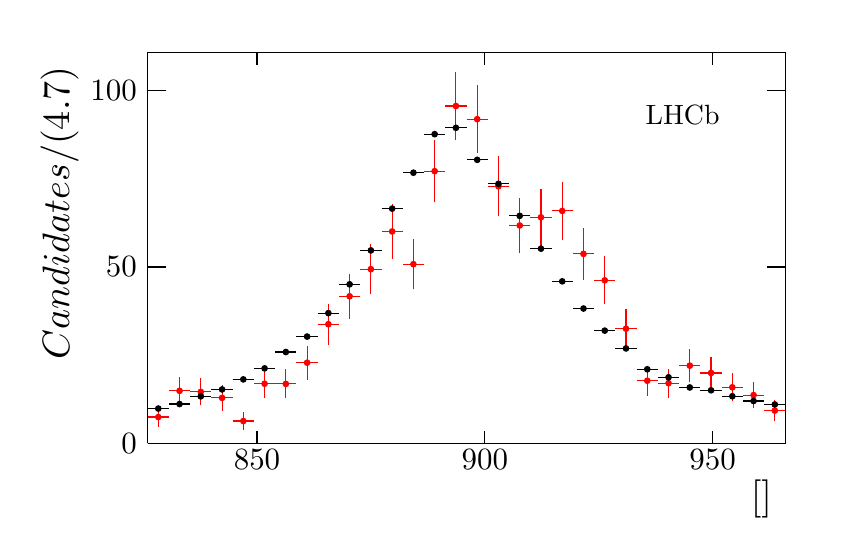
\begin{tikzpicture}
\pgfdeclareplotmark{cross} {
\pgfpathmoveto{\pgfpoint{-0.3\pgfplotmarksize}{\pgfplotmarksize}}
\pgfpathlineto{\pgfpoint{+0.3\pgfplotmarksize}{\pgfplotmarksize}}
\pgfpathlineto{\pgfpoint{+0.3\pgfplotmarksize}{0.3\pgfplotmarksize}}
\pgfpathlineto{\pgfpoint{+1\pgfplotmarksize}{0.3\pgfplotmarksize}}
\pgfpathlineto{\pgfpoint{+1\pgfplotmarksize}{-0.3\pgfplotmarksize}}
\pgfpathlineto{\pgfpoint{+0.3\pgfplotmarksize}{-0.3\pgfplotmarksize}}
\pgfpathlineto{\pgfpoint{+0.3\pgfplotmarksize}{-1.\pgfplotmarksize}}
\pgfpathlineto{\pgfpoint{-0.3\pgfplotmarksize}{-1.\pgfplotmarksize}}
\pgfpathlineto{\pgfpoint{-0.3\pgfplotmarksize}{-0.3\pgfplotmarksize}}
\pgfpathlineto{\pgfpoint{-1.\pgfplotmarksize}{-0.3\pgfplotmarksize}}
\pgfpathlineto{\pgfpoint{-1.\pgfplotmarksize}{0.3\pgfplotmarksize}}
\pgfpathlineto{\pgfpoint{-0.3\pgfplotmarksize}{0.3\pgfplotmarksize}}
\pgfpathclose
\pgfusepathqstroke
}
\pgfdeclareplotmark{cross*} {
\pgfpathmoveto{\pgfpoint{-0.3\pgfplotmarksize}{\pgfplotmarksize}}
\pgfpathlineto{\pgfpoint{+0.3\pgfplotmarksize}{\pgfplotmarksize}}
\pgfpathlineto{\pgfpoint{+0.3\pgfplotmarksize}{0.3\pgfplotmarksize}}
\pgfpathlineto{\pgfpoint{+1\pgfplotmarksize}{0.3\pgfplotmarksize}}
\pgfpathlineto{\pgfpoint{+1\pgfplotmarksize}{-0.3\pgfplotmarksize}}
\pgfpathlineto{\pgfpoint{+0.3\pgfplotmarksize}{-0.3\pgfplotmarksize}}
\pgfpathlineto{\pgfpoint{+0.3\pgfplotmarksize}{-1.\pgfplotmarksize}}
\pgfpathlineto{\pgfpoint{-0.3\pgfplotmarksize}{-1.\pgfplotmarksize}}
\pgfpathlineto{\pgfpoint{-0.3\pgfplotmarksize}{-0.3\pgfplotmarksize}}
\pgfpathlineto{\pgfpoint{-1.\pgfplotmarksize}{-0.3\pgfplotmarksize}}
\pgfpathlineto{\pgfpoint{-1.\pgfplotmarksize}{0.3\pgfplotmarksize}}
\pgfpathlineto{\pgfpoint{-0.3\pgfplotmarksize}{0.3\pgfplotmarksize}}
\pgfpathclose
\pgfusepathqfillstroke
}
\pgfdeclareplotmark{newstar} {
\pgfpathmoveto{\pgfqpoint{0pt}{\pgfplotmarksize}}
\pgfpathlineto{\pgfqpointpolar{44}{0.5\pgfplotmarksize}}
\pgfpathlineto{\pgfqpointpolar{18}{\pgfplotmarksize}}
\pgfpathlineto{\pgfqpointpolar{-20}{0.5\pgfplotmarksize}}
\pgfpathlineto{\pgfqpointpolar{-54}{\pgfplotmarksize}}
\pgfpathlineto{\pgfqpointpolar{-90}{0.5\pgfplotmarksize}}
\pgfpathlineto{\pgfqpointpolar{234}{\pgfplotmarksize}}
\pgfpathlineto{\pgfqpointpolar{198}{0.5\pgfplotmarksize}}
\pgfpathlineto{\pgfqpointpolar{162}{\pgfplotmarksize}}
\pgfpathlineto{\pgfqpointpolar{134}{0.5\pgfplotmarksize}}
\pgfpathclose
\pgfusepathqstroke
}
\pgfdeclareplotmark{newstar*} {
\pgfpathmoveto{\pgfqpoint{0pt}{\pgfplotmarksize}}
\pgfpathlineto{\pgfqpointpolar{44}{0.5\pgfplotmarksize}}
\pgfpathlineto{\pgfqpointpolar{18}{\pgfplotmarksize}}
\pgfpathlineto{\pgfqpointpolar{-20}{0.5\pgfplotmarksize}}
\pgfpathlineto{\pgfqpointpolar{-54}{\pgfplotmarksize}}
\pgfpathlineto{\pgfqpointpolar{-90}{0.5\pgfplotmarksize}}
\pgfpathlineto{\pgfqpointpolar{234}{\pgfplotmarksize}}
\pgfpathlineto{\pgfqpointpolar{198}{0.5\pgfplotmarksize}}
\pgfpathlineto{\pgfqpointpolar{162}{\pgfplotmarksize}}
\pgfpathlineto{\pgfqpointpolar{134}{0.5\pgfplotmarksize}}
\pgfpathclose
\pgfusepathqfillstroke
}
\definecolor{c}{rgb}{1,1,1};
\draw [color=c, fill=c] (0,0) rectangle (10,6.27517);
\draw [color=c, fill=c] (1.4,1.00403) rectangle (9.5,5.96141);
\definecolor{c}{rgb}{0,0,0};
\draw [c] (1.4,1.00403) -- (1.4,5.96141) -- (9.5,5.96141) -- (9.5,1.00403) -- (1.4,1.00403);
\definecolor{c}{rgb}{1,1,1};
\draw [color=c, fill=c] (1.4,1.00403) rectangle (9.5,5.96141);
\definecolor{c}{rgb}{0,0,0};
\draw [c] (1.4,1.00403) -- (1.4,5.96141) -- (9.5,5.96141) -- (9.5,1.00403) -- (1.4,1.00403);
\definecolor{c}{rgb}{1,0,0};
\draw [c,line width=0.4] (1.535,1.21521) -- (1.535,1.33737);
\draw [c,line width=0.4] (1.535,1.33737) -- (1.535,1.45953);
\draw [c,line width=0.4] (1.4,1.33737) -- (1.535,1.33737);
\draw [c,line width=0.4] (1.535,1.33737) -- (1.67,1.33737);
\foreach \P in {(1.535,1.33737)}{\draw[mark options={color=c,fill=c},mark size=2.402402pt,mark=*,mark size=1pt] plot coordinates {\P};}
\draw [c,line width=0.4] (1.805,1.49722) -- (1.805,1.66987);
\draw [c,line width=0.4] (1.805,1.66987) -- (1.805,1.84252);
\draw [c,line width=0.4] (1.67,1.66987) -- (1.805,1.66987);
\draw [c,line width=0.4] (1.805,1.66987) -- (1.94,1.66987);
\foreach \P in {(1.805,1.66987)}{\draw[mark options={color=c,fill=c},mark size=2.402402pt,mark=*,mark size=1pt] plot coordinates {\P};}
\draw [c,line width=0.4] (2.075,1.48566) -- (2.075,1.65658);
\draw [c,line width=0.4] (2.075,1.65658) -- (2.075,1.82749);
\draw [c,line width=0.4] (1.94,1.65658) -- (2.075,1.65658);
\draw [c,line width=0.4] (2.075,1.65658) -- (2.21,1.65658);
\foreach \P in {(2.075,1.65658)}{\draw[mark options={color=c,fill=c},mark size=2.402402pt,mark=*,mark size=1pt] plot coordinates {\P};}
\draw [c,line width=0.4] (2.345,1.41972) -- (2.345,1.58035);
\draw [c,line width=0.4] (2.345,1.58035) -- (2.345,1.74097);
\draw [c,line width=0.4] (2.21,1.58035) -- (2.345,1.58035);
\draw [c,line width=0.4] (2.345,1.58035) -- (2.48,1.58035);
\foreach \P in {(2.345,1.58035)}{\draw[mark options={color=c,fill=c},mark size=2.402402pt,mark=*,mark size=1pt] plot coordinates {\P};}
\draw [c,line width=0.4] (2.615,1.17396) -- (2.615,1.2864);
\draw [c,line width=0.4] (2.615,1.2864) -- (2.615,1.39883);
\draw [c,line width=0.4] (2.48,1.2864) -- (2.615,1.2864);
\draw [c,line width=0.4] (2.615,1.2864) -- (2.75,1.2864);
\foreach \P in {(2.615,1.2864)}{\draw[mark options={color=c,fill=c},mark size=2.402402pt,mark=*,mark size=1pt] plot coordinates {\P};}
\draw [c,line width=0.4] (2.885,1.57625) -- (2.885,1.76025);
\draw [c,line width=0.4] (2.885,1.76025) -- (2.885,1.94424);
\draw [c,line width=0.4] (2.75,1.76025) -- (2.885,1.76025);
\draw [c,line width=0.4] (2.885,1.76025) -- (3.02,1.76025);
\foreach \P in {(2.885,1.76025)}{\draw[mark options={color=c,fill=c},mark size=2.402402pt,mark=*,mark size=1pt] plot coordinates {\P};}
\draw [c,line width=0.4] (3.155,1.57448) -- (3.155,1.75823);
\draw [c,line width=0.4] (3.155,1.75823) -- (3.155,1.94198);
\draw [c,line width=0.4] (3.02,1.75823) -- (3.155,1.75823);
\draw [c,line width=0.4] (3.155,1.75823) -- (3.29,1.75823);
\foreach \P in {(3.155,1.75823)}{\draw[mark options={color=c,fill=c},mark size=2.402402pt,mark=*,mark size=1pt] plot coordinates {\P};}
\draw [c,line width=0.4] (3.425,1.81321) -- (3.425,2.02724);
\draw [c,line width=0.4] (3.425,2.02724) -- (3.425,2.24126);
\draw [c,line width=0.4] (3.29,2.02724) -- (3.425,2.02724);
\draw [c,line width=0.4] (3.425,2.02724) -- (3.56,2.02724);
\foreach \P in {(3.425,2.02724)}{\draw[mark options={color=c,fill=c},mark size=2.402402pt,mark=*,mark size=1pt] plot coordinates {\P};}
\draw [c,line width=0.4] (3.695,2.25571) -- (3.695,2.51587);
\draw [c,line width=0.4] (3.695,2.51587) -- (3.695,2.77603);
\draw [c,line width=0.4] (3.56,2.51587) -- (3.695,2.51587);
\draw [c,line width=0.4] (3.695,2.51587) -- (3.83,2.51587);
\foreach \P in {(3.695,2.51587)}{\draw[mark options={color=c,fill=c},mark size=2.402402pt,mark=*,mark size=1pt] plot coordinates {\P};}
\draw [c,line width=0.4] (3.965,2.58184) -- (3.965,2.87094);
\draw [c,line width=0.4] (3.965,2.87094) -- (3.965,3.16004);
\draw [c,line width=0.4] (3.83,2.87094) -- (3.965,2.87094);
\draw [c,line width=0.4] (3.965,2.87094) -- (4.1,2.87094);
\foreach \P in {(3.965,2.87094)}{\draw[mark options={color=c,fill=c},mark size=2.402402pt,mark=*,mark size=1pt] plot coordinates {\P};}
\draw [c,line width=0.4] (4.235,2.90073) -- (4.235,3.21536);
\draw [c,line width=0.4] (4.235,3.21536) -- (4.235,3.53);
\draw [c,line width=0.4] (4.1,3.21536) -- (4.235,3.21536);
\draw [c,line width=0.4] (4.235,3.21536) -- (4.37,3.21536);
\foreach \P in {(4.235,3.21536)}{\draw[mark options={color=c,fill=c},mark size=2.402402pt,mark=*,mark size=1pt] plot coordinates {\P};}
\draw [c,line width=0.4] (4.505,3.34704) -- (4.505,3.69406);
\draw [c,line width=0.4] (4.505,3.69406) -- (4.505,4.04109);
\draw [c,line width=0.4] (4.37,3.69406) -- (4.505,3.69406);
\draw [c,line width=0.4] (4.505,3.69406) -- (4.64,3.69406);
\foreach \P in {(4.505,3.69406)}{\draw[mark options={color=c,fill=c},mark size=2.402402pt,mark=*,mark size=1pt] plot coordinates {\P};}
\draw [c,line width=0.4] (4.775,2.95942) -- (4.775,3.27852);
\draw [c,line width=0.4] (4.775,3.27852) -- (4.775,3.59762);
\draw [c,line width=0.4] (4.64,3.27852) -- (4.775,3.27852);
\draw [c,line width=0.4] (4.775,3.27852) -- (4.91,3.27852);
\foreach \P in {(4.775,3.27852)}{\draw[mark options={color=c,fill=c},mark size=2.402402pt,mark=*,mark size=1pt] plot coordinates {\P};}
\draw [c,line width=0.4] (5.045,4.06677) -- (5.045,4.46011);
\draw [c,line width=0.4] (5.045,4.46011) -- (5.045,4.85346);
\draw [c,line width=0.4] (4.91,4.46011) -- (5.045,4.46011);
\draw [c,line width=0.4] (5.045,4.46011) -- (5.18,4.46011);
\foreach \P in {(5.045,4.46011)}{\draw[mark options={color=c,fill=c},mark size=2.402402pt,mark=*,mark size=1pt] plot coordinates {\P};}
\draw [c,line width=0.4] (5.315,4.84954) -- (5.315,5.28744);
\draw [c,line width=0.4] (5.315,5.28744) -- (5.315,5.72534);
\draw [c,line width=0.4] (5.18,5.28744) -- (5.315,5.28744);
\draw [c,line width=0.4] (5.315,5.28744) -- (5.45,5.28744);
\foreach \P in {(5.315,5.28744)}{\draw[mark options={color=c,fill=c},mark size=2.402402pt,mark=*,mark size=1pt] plot coordinates {\P};}
\draw [c,line width=0.4] (5.585,4.6908) -- (5.585,5.12006);
\draw [c,line width=0.4] (5.585,5.12006) -- (5.585,5.54932);
\draw [c,line width=0.4] (5.45,5.12006) -- (5.585,5.12006);
\draw [c,line width=0.4] (5.585,5.12006) -- (5.72,5.12006);
\foreach \P in {(5.585,5.12006)}{\draw[mark options={color=c,fill=c},mark size=2.402402pt,mark=*,mark size=1pt] plot coordinates {\P};}
\draw [c,line width=0.4] (5.855,3.88595) -- (5.855,4.26822);
\draw [c,line width=0.4] (5.855,4.26822) -- (5.855,4.65049);
\draw [c,line width=0.4] (5.72,4.26822) -- (5.855,4.26822);
\draw [c,line width=0.4] (5.855,4.26822) -- (5.99,4.26822);
\foreach \P in {(5.855,4.26822)}{\draw[mark options={color=c,fill=c},mark size=2.402402pt,mark=*,mark size=1pt] plot coordinates {\P};}
\draw [c,line width=0.4] (6.125,3.41805) -- (6.125,3.76993);
\draw [c,line width=0.4] (6.125,3.76993) -- (6.125,4.12182);
\draw [c,line width=0.4] (5.99,3.76993) -- (6.125,3.76993);
\draw [c,line width=0.4] (6.125,3.76993) -- (6.26,3.76993);
\foreach \P in {(6.125,3.76993)}{\draw[mark options={color=c,fill=c},mark size=2.402402pt,mark=*,mark size=1pt] plot coordinates {\P};}
\draw [c,line width=0.4] (6.395,3.51549) -- (6.395,3.87393);
\draw [c,line width=0.4] (6.395,3.87393) -- (6.395,4.23237);
\draw [c,line width=0.4] (6.26,3.87393) -- (6.395,3.87393);
\draw [c,line width=0.4] (6.395,3.87393) -- (6.53,3.87393);
\foreach \P in {(6.395,3.87393)}{\draw[mark options={color=c,fill=c},mark size=2.402402pt,mark=*,mark size=1pt] plot coordinates {\P};}
\draw [c,line width=0.4] (6.665,3.5914) -- (6.665,3.95486);
\draw [c,line width=0.4] (6.665,3.95486) -- (6.665,4.31832);
\draw [c,line width=0.4] (6.53,3.95486) -- (6.665,3.95486);
\draw [c,line width=0.4] (6.665,3.95486) -- (6.8,3.95486);
\foreach \P in {(6.665,3.95486)}{\draw[mark options={color=c,fill=c},mark size=2.402402pt,mark=*,mark size=1pt] plot coordinates {\P};}
\draw [c,line width=0.4] (6.935,3.08114) -- (6.935,3.40928);
\draw [c,line width=0.4] (6.935,3.40928) -- (6.935,3.73743);
\draw [c,line width=0.4] (6.8,3.40928) -- (6.935,3.40928);
\draw [c,line width=0.4] (6.935,3.40928) -- (7.07,3.40928);
\foreach \P in {(6.935,3.40928)}{\draw[mark options={color=c,fill=c},mark size=2.402402pt,mark=*,mark size=1pt] plot coordinates {\P};}
\draw [c,line width=0.4] (7.205,2.76932) -- (7.205,3.07371);
\draw [c,line width=0.4] (7.205,3.07371) -- (7.205,3.3781);
\draw [c,line width=0.4] (7.07,3.07371) -- (7.205,3.07371);
\draw [c,line width=0.4] (7.205,3.07371) -- (7.34,3.07371);
\foreach \P in {(7.205,3.07371)}{\draw[mark options={color=c,fill=c},mark size=2.402402pt,mark=*,mark size=1pt] plot coordinates {\P};}
\draw [c,line width=0.4] (7.475,2.2037) -- (7.475,2.45891);
\draw [c,line width=0.4] (7.475,2.45891) -- (7.475,2.71412);
\draw [c,line width=0.4] (7.34,2.45891) -- (7.475,2.45891);
\draw [c,line width=0.4] (7.475,2.45891) -- (7.61,2.45891);
\foreach \P in {(7.475,2.45891)}{\draw[mark options={color=c,fill=c},mark size=2.402402pt,mark=*,mark size=1pt] plot coordinates {\P};}
\draw [c,line width=0.4] (7.745,1.60969) -- (7.745,1.79825);
\draw [c,line width=0.4] (7.745,1.79825) -- (7.745,1.98681);
\draw [c,line width=0.4] (7.61,1.79825) -- (7.745,1.79825);
\draw [c,line width=0.4] (7.745,1.79825) -- (7.88,1.79825);
\foreach \P in {(7.745,1.79825)}{\draw[mark options={color=c,fill=c},mark size=2.402402pt,mark=*,mark size=1pt] plot coordinates {\P};}
\draw [c,line width=0.4] (8.015,1.58243) -- (8.015,1.76728);
\draw [c,line width=0.4] (8.015,1.76728) -- (8.015,1.95213);
\draw [c,line width=0.4] (7.88,1.76728) -- (8.015,1.76728);
\draw [c,line width=0.4] (8.015,1.76728) -- (8.15,1.76728);
\foreach \P in {(8.015,1.76728)}{\draw[mark options={color=c,fill=c},mark size=2.402402pt,mark=*,mark size=1pt] plot coordinates {\P};}
\draw [c,line width=0.4] (8.285,1.7799) -- (8.285,1.99);
\draw [c,line width=0.4] (8.285,1.99) -- (8.285,2.20009);
\draw [c,line width=0.4] (8.15,1.99) -- (8.285,1.99);
\draw [c,line width=0.4] (8.285,1.99) -- (8.42,1.99);
\foreach \P in {(8.285,1.99)}{\draw[mark options={color=c,fill=c},mark size=2.402402pt,mark=*,mark size=1pt] plot coordinates {\P};}
\draw [c,line width=0.4] (8.555,1.69713) -- (8.555,1.89708);
\draw [c,line width=0.4] (8.555,1.89708) -- (8.555,2.09703);
\draw [c,line width=0.4] (8.42,1.89708) -- (8.555,1.89708);
\draw [c,line width=0.4] (8.555,1.89708) -- (8.69,1.89708);
\foreach \P in {(8.555,1.89708)}{\draw[mark options={color=c,fill=c},mark size=2.402402pt,mark=*,mark size=1pt] plot coordinates {\P};}
\draw [c,line width=0.4] (8.825,1.53677) -- (8.825,1.7152);
\draw [c,line width=0.4] (8.825,1.7152) -- (8.825,1.89363);
\draw [c,line width=0.4] (8.69,1.7152) -- (8.825,1.7152);
\draw [c,line width=0.4] (8.825,1.7152) -- (8.96,1.7152);
\foreach \P in {(8.825,1.7152)}{\draw[mark options={color=c,fill=c},mark size=2.402402pt,mark=*,mark size=1pt] plot coordinates {\P};}
\draw [c,line width=0.4] (9.095,1.45023) -- (9.095,1.61571);
\draw [c,line width=0.4] (9.095,1.61571) -- (9.095,1.78118);
\draw [c,line width=0.4] (8.96,1.61571) -- (9.095,1.61571);
\draw [c,line width=0.4] (9.095,1.61571) -- (9.23,1.61571);
\foreach \P in {(9.095,1.61571)}{\draw[mark options={color=c,fill=c},mark size=2.402402pt,mark=*,mark size=1pt] plot coordinates {\P};}
\draw [c,line width=0.4] (9.365,1.28266) -- (9.365,1.41895);
\draw [c,line width=0.4] (9.365,1.41895) -- (9.365,1.55524);
\draw [c,line width=0.4] (9.23,1.41895) -- (9.365,1.41895);
\draw [c,line width=0.4] (9.365,1.41895) -- (9.5,1.41895);
\foreach \P in {(9.365,1.41895)}{\draw[mark options={color=c,fill=c},mark size=2.402402pt,mark=*,mark size=1pt] plot coordinates {\P};}
\definecolor{c}{rgb}{0,0,0};
\draw [c,line width=0.4] (1.4,1.00403) -- (9.5,1.00403);
\draw [anchor= east] (9.5,0.301208) node[scale=1.37879, rotate=0]{$\mkpi [\mevcc]$};
\draw [c,line width=0.4] (2.78857,1.15651) -- (2.78857,1.00403);
\draw [c,line width=0.4] (5.68143,1.15651) -- (5.68143,1.00403);
\draw [c,line width=0.4] (8.57429,1.15651) -- (8.57429,1.00403);
\draw [c,line width=0.4] (2.78857,1.15651) -- (2.78857,1.00403);
\draw [c,line width=0.4] (8.57429,1.15651) -- (8.57429,1.00403);
\draw [anchor=base] (2.78857,0.665168) node[scale=1.11794, rotate=0]{850};
\draw [anchor=base] (5.68143,0.665168) node[scale=1.11794, rotate=0]{900};
\draw [anchor=base] (8.57429,0.665168) node[scale=1.11794, rotate=0]{950};
\draw [c,line width=0.4] (1.4,5.96141) -- (9.5,5.96141);
\draw [c,line width=0.4] (2.78857,5.80892) -- (2.78857,5.96141);
\draw [c,line width=0.4] (5.68143,5.80892) -- (5.68143,5.96141);
\draw [c,line width=0.4] (8.57429,5.80892) -- (8.57429,5.96141);
\draw [c,line width=0.4] (2.78857,5.80892) -- (2.78857,5.96141);
\draw [c,line width=0.4] (8.57429,5.80892) -- (8.57429,5.96141);
\draw [c,line width=0.4] (1.4,1.00403) -- (1.4,5.96141);
\draw [anchor= east] (0.28,5.96141) node[scale=1.37879, rotate=90]{$\text{Candidates} / (4.7 \mevcc)$};
\draw [c,line width=0.4] (1.637,1.00403) -- (1.4,1.00403);
\draw [c,line width=0.4] (1.637,3.24241) -- (1.4,3.24241);
\draw [c,line width=0.4] (1.637,5.48079) -- (1.4,5.48079);
\draw [c,line width=0.4] (1.637,5.48079) -- (1.4,5.48079);
\draw [anchor= east] (1.4,1.00403) node[scale=1.11794, rotate=0]{0};
\draw [anchor= east] (1.4,3.24241) node[scale=1.11794, rotate=0]{50};
\draw [anchor= east] (1.4,5.48079) node[scale=1.11794, rotate=0]{100};
\draw [c,line width=0.4] (9.5,1.00403) -- (9.5,5.96141);
\draw [c,line width=0.4] (9.263,1.00403) -- (9.5,1.00403);
\draw [c,line width=0.4] (9.263,3.24241) -- (9.5,3.24241);
\draw [c,line width=0.4] (9.263,5.48079) -- (9.5,5.48079);
\draw [c,line width=0.4] (9.263,5.48079) -- (9.5,5.48079);
\draw [c,line width=0.4] (1.535,1.4337) -- (1.535,1.44495);
\draw [c,line width=0.4] (1.535,1.44495) -- (1.535,1.45621);
\draw [c,line width=0.4] (1.4,1.44495) -- (1.535,1.44495);
\draw [c,line width=0.4] (1.535,1.44495) -- (1.67,1.44495);
\foreach \P in {(1.535,1.44495)}{\draw[mark options={color=c,fill=c},mark size=2.402402pt,mark=*,mark size=1pt] plot coordinates {\P};}
\draw [c,line width=0.4] (1.805,1.49052) -- (1.805,1.50248);
\draw [c,line width=0.4] (1.805,1.50248) -- (1.805,1.51444);
\draw [c,line width=0.4] (1.67,1.50248) -- (1.805,1.50248);
\draw [c,line width=0.4] (1.805,1.50248) -- (1.94,1.50248);
\foreach \P in {(1.805,1.50248)}{\draw[mark options={color=c,fill=c},mark size=2.402402pt,mark=*,mark size=1pt] plot coordinates {\P};}
\draw [c,line width=0.4] (2.075,1.58698) -- (2.075,1.60006);
\draw [c,line width=0.4] (2.075,1.60006) -- (2.075,1.61314);
\draw [c,line width=0.4] (1.94,1.60006) -- (2.075,1.60006);
\draw [c,line width=0.4] (2.075,1.60006) -- (2.21,1.60006);
\foreach \P in {(2.075,1.60006)}{\draw[mark options={color=c,fill=c},mark size=2.402402pt,mark=*,mark size=1pt] plot coordinates {\P};}
\draw [c,line width=0.4] (2.345,1.67397) -- (2.345,1.68798);
\draw [c,line width=0.4] (2.345,1.68798) -- (2.345,1.702);
\draw [c,line width=0.4] (2.21,1.68798) -- (2.345,1.68798);
\draw [c,line width=0.4] (2.345,1.68798) -- (2.48,1.68798);
\foreach \P in {(2.345,1.68798)}{\draw[mark options={color=c,fill=c},mark size=2.402402pt,mark=*,mark size=1pt] plot coordinates {\P};}
\draw [c,line width=0.4] (2.615,1.80015) -- (2.615,1.81541);
\draw [c,line width=0.4] (2.615,1.81541) -- (2.615,1.83067);
\draw [c,line width=0.4] (2.48,1.81541) -- (2.615,1.81541);
\draw [c,line width=0.4] (2.615,1.81541) -- (2.75,1.81541);
\foreach \P in {(2.615,1.81541)}{\draw[mark options={color=c,fill=c},mark size=2.402402pt,mark=*,mark size=1pt] plot coordinates {\P};}
\draw [c,line width=0.4] (2.885,1.93874) -- (2.885,1.95527);
\draw [c,line width=0.4] (2.885,1.95527) -- (2.885,1.9718);
\draw [c,line width=0.4] (2.75,1.95527) -- (2.885,1.95527);
\draw [c,line width=0.4] (2.885,1.95527) -- (3.02,1.95527);
\foreach \P in {(2.885,1.95527)}{\draw[mark options={color=c,fill=c},mark size=2.402402pt,mark=*,mark size=1pt] plot coordinates {\P};}
\draw [c,line width=0.4] (3.155,2.14466) -- (3.155,2.1629);
\draw [c,line width=0.4] (3.155,2.1629) -- (3.155,2.18114);
\draw [c,line width=0.4] (3.02,2.1629) -- (3.155,2.1629);
\draw [c,line width=0.4] (3.155,2.1629) -- (3.29,2.1629);
\foreach \P in {(3.155,2.1629)}{\draw[mark options={color=c,fill=c},mark size=2.402402pt,mark=*,mark size=1pt] plot coordinates {\P};}
\draw [c,line width=0.4] (3.425,2.33954) -- (3.425,2.35926);
\draw [c,line width=0.4] (3.425,2.35926) -- (3.425,2.37899);
\draw [c,line width=0.4] (3.29,2.35926) -- (3.425,2.35926);
\draw [c,line width=0.4] (3.425,2.35926) -- (3.56,2.35926);
\foreach \P in {(3.425,2.35926)}{\draw[mark options={color=c,fill=c},mark size=2.402402pt,mark=*,mark size=1pt] plot coordinates {\P};}
\draw [c,line width=0.4] (3.695,2.6353) -- (3.695,2.65709);
\draw [c,line width=0.4] (3.695,2.65709) -- (3.695,2.67888);
\draw [c,line width=0.4] (3.56,2.65709) -- (3.695,2.65709);
\draw [c,line width=0.4] (3.695,2.65709) -- (3.83,2.65709);
\foreach \P in {(3.695,2.65709)}{\draw[mark options={color=c,fill=c},mark size=2.402402pt,mark=*,mark size=1pt] plot coordinates {\P};}
\draw [c,line width=0.4] (3.965,2.99871) -- (3.965,3.02278);
\draw [c,line width=0.4] (3.965,3.02278) -- (3.965,3.04686);
\draw [c,line width=0.4] (3.83,3.02278) -- (3.965,3.02278);
\draw [c,line width=0.4] (3.965,3.02278) -- (4.1,3.02278);
\foreach \P in {(3.965,3.02278)}{\draw[mark options={color=c,fill=c},mark size=2.402402pt,mark=*,mark size=1pt] plot coordinates {\P};}
\draw [c,line width=0.4] (4.235,3.42701) -- (4.235,3.45353);
\draw [c,line width=0.4] (4.235,3.45353) -- (4.235,3.48005);
\draw [c,line width=0.4] (4.1,3.45353) -- (4.235,3.45353);
\draw [c,line width=0.4] (4.235,3.45353) -- (4.37,3.45353);
\foreach \P in {(4.235,3.45353)}{\draw[mark options={color=c,fill=c},mark size=2.402402pt,mark=*,mark size=1pt] plot coordinates {\P};}
\draw [c,line width=0.4] (4.505,3.95471) -- (4.505,3.98396);
\draw [c,line width=0.4] (4.505,3.98396) -- (4.505,4.01321);
\draw [c,line width=0.4] (4.37,3.98396) -- (4.505,3.98396);
\draw [c,line width=0.4] (4.505,3.98396) -- (4.64,3.98396);
\foreach \P in {(4.505,3.98396)}{\draw[mark options={color=c,fill=c},mark size=2.402402pt,mark=*,mark size=1pt] plot coordinates {\P};}
\draw [c,line width=0.4] (4.775,4.40867) -- (4.775,4.44008);
\draw [c,line width=0.4] (4.775,4.44008) -- (4.775,4.4715);
\draw [c,line width=0.4] (4.64,4.44008) -- (4.775,4.44008);
\draw [c,line width=0.4] (4.775,4.44008) -- (4.91,4.44008);
\foreach \P in {(4.775,4.44008)}{\draw[mark options={color=c,fill=c},mark size=2.402402pt,mark=*,mark size=1pt] plot coordinates {\P};}
\draw [c,line width=0.4] (5.045,4.89615) -- (5.045,4.92972);
\draw [c,line width=0.4] (5.045,4.92972) -- (5.045,4.9633);
\draw [c,line width=0.4] (4.91,4.92972) -- (5.045,4.92972);
\draw [c,line width=0.4] (5.045,4.92972) -- (5.18,4.92972);
\foreach \P in {(5.045,4.92972)}{\draw[mark options={color=c,fill=c},mark size=2.402402pt,mark=*,mark size=1pt] plot coordinates {\P};}
\draw [c,line width=0.4] (5.315,4.9763) -- (5.315,5.01022);
\draw [c,line width=0.4] (5.315,5.01022) -- (5.315,5.04414);
\draw [c,line width=0.4] (5.18,5.01022) -- (5.315,5.01022);
\draw [c,line width=0.4] (5.315,5.01022) -- (5.45,5.01022);
\foreach \P in {(5.315,5.01022)}{\draw[mark options={color=c,fill=c},mark size=2.402402pt,mark=*,mark size=1pt] plot coordinates {\P};}
\draw [c,line width=0.4] (5.585,4.57166) -- (5.585,4.60381);
\draw [c,line width=0.4] (5.585,4.60381) -- (5.585,4.63596);
\draw [c,line width=0.4] (5.45,4.60381) -- (5.585,4.60381);
\draw [c,line width=0.4] (5.585,4.60381) -- (5.72,4.60381);
\foreach \P in {(5.585,4.60381)}{\draw[mark options={color=c,fill=c},mark size=2.402402pt,mark=*,mark size=1pt] plot coordinates {\P};}
\draw [c,line width=0.4] (5.855,4.26804) -- (5.855,4.2988);
\draw [c,line width=0.4] (5.855,4.2988) -- (5.855,4.32956);
\draw [c,line width=0.4] (5.72,4.2988) -- (5.855,4.2988);
\draw [c,line width=0.4] (5.855,4.2988) -- (5.99,4.2988);
\foreach \P in {(5.855,4.2988)}{\draw[mark options={color=c,fill=c},mark size=2.402402pt,mark=*,mark size=1pt] plot coordinates {\P};}
\draw [c,line width=0.4] (6.125,3.86347) -- (6.125,3.89227);
\draw [c,line width=0.4] (6.125,3.89227) -- (6.125,3.92107);
\draw [c,line width=0.4] (5.99,3.89227) -- (6.125,3.89227);
\draw [c,line width=0.4] (6.125,3.89227) -- (6.26,3.89227);
\foreach \P in {(6.125,3.89227)}{\draw[mark options={color=c,fill=c},mark size=2.402402pt,mark=*,mark size=1pt] plot coordinates {\P};}
\draw [c,line width=0.4] (6.395,3.44879) -- (6.395,3.47543);
\draw [c,line width=0.4] (6.395,3.47543) -- (6.395,3.50207);
\draw [c,line width=0.4] (6.26,3.47543) -- (6.395,3.47543);
\draw [c,line width=0.4] (6.395,3.47543) -- (6.53,3.47543);
\foreach \P in {(6.395,3.47543)}{\draw[mark options={color=c,fill=c},mark size=2.402402pt,mark=*,mark size=1pt] plot coordinates {\P};}
\draw [c,line width=0.4] (6.665,3.0363) -- (6.665,3.0606);
\draw [c,line width=0.4] (6.665,3.0606) -- (6.665,3.0849);
\draw [c,line width=0.4] (6.53,3.0606) -- (6.665,3.0606);
\draw [c,line width=0.4] (6.665,3.0606) -- (6.8,3.0606);
\foreach \P in {(6.665,3.0606)}{\draw[mark options={color=c,fill=c},mark size=2.402402pt,mark=*,mark size=1pt] plot coordinates {\P};}
\draw [c,line width=0.4] (6.935,2.69321) -- (6.935,2.71538);
\draw [c,line width=0.4] (6.935,2.71538) -- (6.935,2.73755);
\draw [c,line width=0.4] (6.8,2.71538) -- (6.935,2.71538);
\draw [c,line width=0.4] (6.935,2.71538) -- (7.07,2.71538);
\foreach \P in {(6.935,2.71538)}{\draw[mark options={color=c,fill=c},mark size=2.402402pt,mark=*,mark size=1pt] plot coordinates {\P};}
\draw [c,line width=0.4] (7.205,2.41446) -- (7.205,2.43473);
\draw [c,line width=0.4] (7.205,2.43473) -- (7.205,2.455);
\draw [c,line width=0.4] (7.07,2.43473) -- (7.205,2.43473);
\draw [c,line width=0.4] (7.205,2.43473) -- (7.34,2.43473);
\foreach \P in {(7.205,2.43473)}{\draw[mark options={color=c,fill=c},mark size=2.402402pt,mark=*,mark size=1pt] plot coordinates {\P};}
\draw [c,line width=0.4] (7.475,2.18984) -- (7.475,2.20844);
\draw [c,line width=0.4] (7.475,2.20844) -- (7.475,2.22703);
\draw [c,line width=0.4] (7.34,2.20844) -- (7.475,2.20844);
\draw [c,line width=0.4] (7.475,2.20844) -- (7.61,2.20844);
\foreach \P in {(7.475,2.20844)}{\draw[mark options={color=c,fill=c},mark size=2.402402pt,mark=*,mark size=1pt] plot coordinates {\P};}
\draw [c,line width=0.4] (7.745,1.92756) -- (7.745,1.94399);
\draw [c,line width=0.4] (7.745,1.94399) -- (7.745,1.96042);
\draw [c,line width=0.4] (7.61,1.94399) -- (7.745,1.94399);
\draw [c,line width=0.4] (7.745,1.94399) -- (7.88,1.94399);
\foreach \P in {(7.745,1.94399)}{\draw[mark options={color=c,fill=c},mark size=2.402402pt,mark=*,mark size=1pt] plot coordinates {\P};}
\draw [c,line width=0.4] (8.015,1.82634) -- (8.015,1.84186);
\draw [c,line width=0.4] (8.015,1.84186) -- (8.015,1.85737);
\draw [c,line width=0.4] (7.88,1.84186) -- (8.015,1.84186);
\draw [c,line width=0.4] (8.015,1.84186) -- (8.15,1.84186);
\foreach \P in {(8.015,1.84186)}{\draw[mark options={color=c,fill=c},mark size=2.402402pt,mark=*,mark size=1pt] plot coordinates {\P};}
\draw [c,line width=0.4] (8.285,1.69859) -- (8.285,1.71285);
\draw [c,line width=0.4] (8.285,1.71285) -- (8.285,1.72712);
\draw [c,line width=0.4] (8.15,1.71285) -- (8.285,1.71285);
\draw [c,line width=0.4] (8.285,1.71285) -- (8.42,1.71285);
\foreach \P in {(8.285,1.71285)}{\draw[mark options={color=c,fill=c},mark size=2.402402pt,mark=*,mark size=1pt] plot coordinates {\P};}
\draw [c,line width=0.4] (8.555,1.66293) -- (8.555,1.67683);
\draw [c,line width=0.4] (8.555,1.67683) -- (8.555,1.69073);
\draw [c,line width=0.4] (8.42,1.67683) -- (8.555,1.67683);
\draw [c,line width=0.4] (8.555,1.67683) -- (8.69,1.67683);
\foreach \P in {(8.555,1.67683)}{\draw[mark options={color=c,fill=c},mark size=2.402402pt,mark=*,mark size=1pt] plot coordinates {\P};}
\draw [c,line width=0.4] (8.825,1.58811) -- (8.825,1.60121);
\draw [c,line width=0.4] (8.825,1.60121) -- (8.825,1.6143);
\draw [c,line width=0.4] (8.69,1.60121) -- (8.825,1.60121);
\draw [c,line width=0.4] (8.825,1.60121) -- (8.96,1.60121);
\foreach \P in {(8.825,1.60121)}{\draw[mark options={color=c,fill=c},mark size=2.402402pt,mark=*,mark size=1pt] plot coordinates {\P};}
\draw [c,line width=0.4] (9.095,1.52849) -- (9.095,1.54091);
\draw [c,line width=0.4] (9.095,1.54091) -- (9.095,1.55332);
\draw [c,line width=0.4] (8.96,1.54091) -- (9.095,1.54091);
\draw [c,line width=0.4] (9.095,1.54091) -- (9.23,1.54091);
\foreach \P in {(9.095,1.54091)}{\draw[mark options={color=c,fill=c},mark size=2.402402pt,mark=*,mark size=1pt] plot coordinates {\P};}
\draw [c,line width=0.4] (9.365,1.48526) -- (9.365,1.49716);
\draw [c,line width=0.4] (9.365,1.49716) -- (9.365,1.50906);
\draw [c,line width=0.4] (9.23,1.49716) -- (9.365,1.49716);
\draw [c,line width=0.4] (9.365,1.49716) -- (9.5,1.49716);
\foreach \P in {(9.365,1.49716)}{\draw[mark options={color=c,fill=c},mark size=2.402402pt,mark=*,mark size=1pt] plot coordinates {\P};}
\draw [anchor= west] (7.6,5.17701) node[scale=1.00614, rotate=0]{LHCb};
\end{tikzpicture}
}
    \caption{}
    \label{mkpiPlot_eff}
  \end{subfigure}
  \begin{subfigure}{0.5\textwidth}
    \tikzsetnextfilename{eff_corrected_raw_mdau1} 
    \scalebox{0.65}{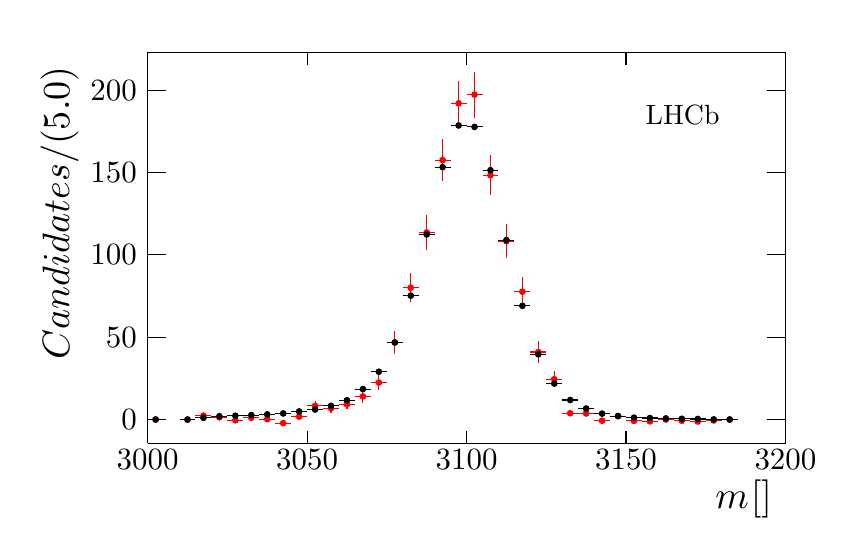
\begin{tikzpicture}
\pgfdeclareplotmark{cross} {
\pgfpathmoveto{\pgfpoint{-0.3\pgfplotmarksize}{\pgfplotmarksize}}
\pgfpathlineto{\pgfpoint{+0.3\pgfplotmarksize}{\pgfplotmarksize}}
\pgfpathlineto{\pgfpoint{+0.3\pgfplotmarksize}{0.3\pgfplotmarksize}}
\pgfpathlineto{\pgfpoint{+1\pgfplotmarksize}{0.3\pgfplotmarksize}}
\pgfpathlineto{\pgfpoint{+1\pgfplotmarksize}{-0.3\pgfplotmarksize}}
\pgfpathlineto{\pgfpoint{+0.3\pgfplotmarksize}{-0.3\pgfplotmarksize}}
\pgfpathlineto{\pgfpoint{+0.3\pgfplotmarksize}{-1.\pgfplotmarksize}}
\pgfpathlineto{\pgfpoint{-0.3\pgfplotmarksize}{-1.\pgfplotmarksize}}
\pgfpathlineto{\pgfpoint{-0.3\pgfplotmarksize}{-0.3\pgfplotmarksize}}
\pgfpathlineto{\pgfpoint{-1.\pgfplotmarksize}{-0.3\pgfplotmarksize}}
\pgfpathlineto{\pgfpoint{-1.\pgfplotmarksize}{0.3\pgfplotmarksize}}
\pgfpathlineto{\pgfpoint{-0.3\pgfplotmarksize}{0.3\pgfplotmarksize}}
\pgfpathclose
\pgfusepathqstroke
}
\pgfdeclareplotmark{cross*} {
\pgfpathmoveto{\pgfpoint{-0.3\pgfplotmarksize}{\pgfplotmarksize}}
\pgfpathlineto{\pgfpoint{+0.3\pgfplotmarksize}{\pgfplotmarksize}}
\pgfpathlineto{\pgfpoint{+0.3\pgfplotmarksize}{0.3\pgfplotmarksize}}
\pgfpathlineto{\pgfpoint{+1\pgfplotmarksize}{0.3\pgfplotmarksize}}
\pgfpathlineto{\pgfpoint{+1\pgfplotmarksize}{-0.3\pgfplotmarksize}}
\pgfpathlineto{\pgfpoint{+0.3\pgfplotmarksize}{-0.3\pgfplotmarksize}}
\pgfpathlineto{\pgfpoint{+0.3\pgfplotmarksize}{-1.\pgfplotmarksize}}
\pgfpathlineto{\pgfpoint{-0.3\pgfplotmarksize}{-1.\pgfplotmarksize}}
\pgfpathlineto{\pgfpoint{-0.3\pgfplotmarksize}{-0.3\pgfplotmarksize}}
\pgfpathlineto{\pgfpoint{-1.\pgfplotmarksize}{-0.3\pgfplotmarksize}}
\pgfpathlineto{\pgfpoint{-1.\pgfplotmarksize}{0.3\pgfplotmarksize}}
\pgfpathlineto{\pgfpoint{-0.3\pgfplotmarksize}{0.3\pgfplotmarksize}}
\pgfpathclose
\pgfusepathqfillstroke
}
\pgfdeclareplotmark{newstar} {
\pgfpathmoveto{\pgfqpoint{0pt}{\pgfplotmarksize}}
\pgfpathlineto{\pgfqpointpolar{44}{0.5\pgfplotmarksize}}
\pgfpathlineto{\pgfqpointpolar{18}{\pgfplotmarksize}}
\pgfpathlineto{\pgfqpointpolar{-20}{0.5\pgfplotmarksize}}
\pgfpathlineto{\pgfqpointpolar{-54}{\pgfplotmarksize}}
\pgfpathlineto{\pgfqpointpolar{-90}{0.5\pgfplotmarksize}}
\pgfpathlineto{\pgfqpointpolar{234}{\pgfplotmarksize}}
\pgfpathlineto{\pgfqpointpolar{198}{0.5\pgfplotmarksize}}
\pgfpathlineto{\pgfqpointpolar{162}{\pgfplotmarksize}}
\pgfpathlineto{\pgfqpointpolar{134}{0.5\pgfplotmarksize}}
\pgfpathclose
\pgfusepathqstroke
}
\pgfdeclareplotmark{newstar*} {
\pgfpathmoveto{\pgfqpoint{0pt}{\pgfplotmarksize}}
\pgfpathlineto{\pgfqpointpolar{44}{0.5\pgfplotmarksize}}
\pgfpathlineto{\pgfqpointpolar{18}{\pgfplotmarksize}}
\pgfpathlineto{\pgfqpointpolar{-20}{0.5\pgfplotmarksize}}
\pgfpathlineto{\pgfqpointpolar{-54}{\pgfplotmarksize}}
\pgfpathlineto{\pgfqpointpolar{-90}{0.5\pgfplotmarksize}}
\pgfpathlineto{\pgfqpointpolar{234}{\pgfplotmarksize}}
\pgfpathlineto{\pgfqpointpolar{198}{0.5\pgfplotmarksize}}
\pgfpathlineto{\pgfqpointpolar{162}{\pgfplotmarksize}}
\pgfpathlineto{\pgfqpointpolar{134}{0.5\pgfplotmarksize}}
\pgfpathclose
\pgfusepathqfillstroke
}
\definecolor{c}{rgb}{1,1,1};
\draw [color=c, fill=c] (0,0) rectangle (10,6.27517);
\draw [color=c, fill=c] (1.4,1.00403) rectangle (9.5,5.96141);
\definecolor{c}{rgb}{0,0,0};
\draw [c] (1.4,1.00403) -- (1.4,5.96141) -- (9.5,5.96141) -- (9.5,1.00403) -- (1.4,1.00403);
\definecolor{c}{rgb}{1,1,1};
\draw [color=c, fill=c] (1.4,1.00403) rectangle (9.5,5.96141);
\definecolor{c}{rgb}{0,0,0};
\draw [c] (1.4,1.00403) -- (1.4,5.96141) -- (9.5,5.96141) -- (9.5,1.00403) -- (1.4,1.00403);
\definecolor{c}{rgb}{1,0,0};
\draw [c,line width=0.4] (1.50125,1.30263) -- (1.50125,1.30542);
\draw [c,line width=0.4] (1.50125,1.30542) -- (1.50125,1.30821);
\draw [c,line width=0.4] (1.4,1.30542) -- (1.50125,1.30542);
\draw [c,line width=0.4] (1.50125,1.30542) -- (1.6025,1.30542);
\foreach \P in {(1.50125,1.30542)}{\draw[mark options={color=c,fill=c},mark size=2.402402pt,mark=*,mark size=1pt] plot coordinates {\P};}
\draw [c,line width=0.4] (1.90625,1.29609) -- (1.90625,1.3033);
\draw [c,line width=0.4] (1.90625,1.3033) -- (1.90625,1.31052);
\draw [c,line width=0.4] (1.805,1.3033) -- (1.90625,1.3033);
\draw [c,line width=0.4] (1.90625,1.3033) -- (2.0075,1.3033);
\foreach \P in {(1.90625,1.3033)}{\draw[mark options={color=c,fill=c},mark size=2.402402pt,mark=*,mark size=1pt] plot coordinates {\P};}
\draw [c,line width=0.4] (2.10875,1.32351) -- (2.10875,1.35585);
\draw [c,line width=0.4] (2.10875,1.35585) -- (2.10875,1.3882);
\draw [c,line width=0.4] (2.0075,1.35585) -- (2.10875,1.35585);
\draw [c,line width=0.4] (2.10875,1.35585) -- (2.21,1.35585);
\foreach \P in {(2.10875,1.35585)}{\draw[mark options={color=c,fill=c},mark size=2.402402pt,mark=*,mark size=1pt] plot coordinates {\P};}
\draw [c,line width=0.4] (2.31125,1.30958) -- (2.31125,1.33376);
\draw [c,line width=0.4] (2.31125,1.33376) -- (2.31125,1.35794);
\draw [c,line width=0.4] (2.21,1.33376) -- (2.31125,1.33376);
\draw [c,line width=0.4] (2.31125,1.33376) -- (2.4125,1.33376);
\foreach \P in {(2.31125,1.33376)}{\draw[mark options={color=c,fill=c},mark size=2.402402pt,mark=*,mark size=1pt] plot coordinates {\P};}
\draw [c,line width=0.4] (2.51375,1.28158) -- (2.51375,1.29593);
\draw [c,line width=0.4] (2.51375,1.29593) -- (2.51375,1.31029);
\draw [c,line width=0.4] (2.4125,1.29593) -- (2.51375,1.29593);
\draw [c,line width=0.4] (2.51375,1.29593) -- (2.615,1.29593);
\foreach \P in {(2.51375,1.29593)}{\draw[mark options={color=c,fill=c},mark size=2.402402pt,mark=*,mark size=1pt] plot coordinates {\P};}
\draw [c,line width=0.4] (2.71625,1.30607) -- (2.71625,1.32724);
\draw [c,line width=0.4] (2.71625,1.32724) -- (2.71625,1.34841);
\draw [c,line width=0.4] (2.615,1.32724) -- (2.71625,1.32724);
\draw [c,line width=0.4] (2.71625,1.32724) -- (2.8175,1.32724);
\foreach \P in {(2.71625,1.32724)}{\draw[mark options={color=c,fill=c},mark size=2.402402pt,mark=*,mark size=1pt] plot coordinates {\P};}
\draw [c,line width=0.4] (2.91875,1.30066) -- (2.91875,1.30973);
\draw [c,line width=0.4] (2.91875,1.30973) -- (2.91875,1.31879);
\draw [c,line width=0.4] (2.8175,1.30973) -- (2.91875,1.30973);
\draw [c,line width=0.4] (2.91875,1.30973) -- (3.02,1.30973);
\foreach \P in {(2.91875,1.30973)}{\draw[mark options={color=c,fill=c},mark size=2.402402pt,mark=*,mark size=1pt] plot coordinates {\P};}
\draw [c,line width=0.4] (3.12125,1.22885) -- (3.12125,1.25984);
\draw [c,line width=0.4] (3.12125,1.25984) -- (3.12125,1.29084);
\draw [c,line width=0.4] (3.02,1.25984) -- (3.12125,1.25984);
\draw [c,line width=0.4] (3.12125,1.25984) -- (3.2225,1.25984);
\foreach \P in {(3.12125,1.25984)}{\draw[mark options={color=c,fill=c},mark size=2.402402pt,mark=*,mark size=1pt] plot coordinates {\P};}
\draw [c,line width=0.4] (3.32375,1.31427) -- (3.32375,1.34164);
\draw [c,line width=0.4] (3.32375,1.34164) -- (3.32375,1.36902);
\draw [c,line width=0.4] (3.2225,1.34164) -- (3.32375,1.34164);
\draw [c,line width=0.4] (3.32375,1.34164) -- (3.425,1.34164);
\foreach \P in {(3.32375,1.34164)}{\draw[mark options={color=c,fill=c},mark size=2.402402pt,mark=*,mark size=1pt] plot coordinates {\P};}
\draw [c,line width=0.4] (3.52625,1.41873) -- (3.52625,1.47888);
\draw [c,line width=0.4] (3.52625,1.47888) -- (3.52625,1.53903);
\draw [c,line width=0.4] (3.425,1.47888) -- (3.52625,1.47888);
\draw [c,line width=0.4] (3.52625,1.47888) -- (3.6275,1.47888);
\foreach \P in {(3.52625,1.47888)}{\draw[mark options={color=c,fill=c},mark size=2.402402pt,mark=*,mark size=1pt] plot coordinates {\P};}
\draw [c,line width=0.4] (3.72875,1.39417) -- (3.72875,1.44886);
\draw [c,line width=0.4] (3.72875,1.44886) -- (3.72875,1.50354);
\draw [c,line width=0.4] (3.6275,1.44886) -- (3.72875,1.44886);
\draw [c,line width=0.4] (3.72875,1.44886) -- (3.83,1.44886);
\foreach \P in {(3.72875,1.44886)}{\draw[mark options={color=c,fill=c},mark size=2.402402pt,mark=*,mark size=1pt] plot coordinates {\P};}
\draw [c,line width=0.4] (3.93125,1.43498) -- (3.93125,1.49844);
\draw [c,line width=0.4] (3.93125,1.49844) -- (3.93125,1.5619);
\draw [c,line width=0.4] (3.83,1.49844) -- (3.93125,1.49844);
\draw [c,line width=0.4] (3.93125,1.49844) -- (4.0325,1.49844);
\foreach \P in {(3.93125,1.49844)}{\draw[mark options={color=c,fill=c},mark size=2.402402pt,mark=*,mark size=1pt] plot coordinates {\P};}
\draw [c,line width=0.4] (4.13375,1.52091) -- (4.13375,1.59922);
\draw [c,line width=0.4] (4.13375,1.59922) -- (4.13375,1.67754);
\draw [c,line width=0.4] (4.0325,1.59922) -- (4.13375,1.59922);
\draw [c,line width=0.4] (4.13375,1.59922) -- (4.235,1.59922);
\foreach \P in {(4.13375,1.59922)}{\draw[mark options={color=c,fill=c},mark size=2.402402pt,mark=*,mark size=1pt] plot coordinates {\P};}
\draw [c,line width=0.4] (4.33625,1.67561) -- (4.33625,1.77461);
\draw [c,line width=0.4] (4.33625,1.77461) -- (4.33625,1.8736);
\draw [c,line width=0.4] (4.235,1.77461) -- (4.33625,1.77461);
\draw [c,line width=0.4] (4.33625,1.77461) -- (4.4375,1.77461);
\foreach \P in {(4.33625,1.77461)}{\draw[mark options={color=c,fill=c},mark size=2.402402pt,mark=*,mark size=1pt] plot coordinates {\P};}
\draw [c,line width=0.4] (4.53875,2.14103) -- (4.53875,2.28403);
\draw [c,line width=0.4] (4.53875,2.28403) -- (4.53875,2.42702);
\draw [c,line width=0.4] (4.4375,2.28403) -- (4.53875,2.28403);
\draw [c,line width=0.4] (4.53875,2.28403) -- (4.64,2.28403);
\foreach \P in {(4.53875,2.28403)}{\draw[mark options={color=c,fill=c},mark size=2.402402pt,mark=*,mark size=1pt] plot coordinates {\P};}
\draw [c,line width=0.4] (4.74125,2.79202) -- (4.74125,2.97904);
\draw [c,line width=0.4] (4.74125,2.97904) -- (4.74125,3.16605);
\draw [c,line width=0.4] (4.64,2.97904) -- (4.74125,2.97904);
\draw [c,line width=0.4] (4.74125,2.97904) -- (4.8425,2.97904);
\foreach \P in {(4.74125,2.97904)}{\draw[mark options={color=c,fill=c},mark size=2.402402pt,mark=*,mark size=1pt] plot coordinates {\P};}
\draw [c,line width=0.4] (4.94375,3.45838) -- (4.94375,3.68121);
\draw [c,line width=0.4] (4.94375,3.68121) -- (4.94375,3.90404);
\draw [c,line width=0.4] (4.8425,3.68121) -- (4.94375,3.68121);
\draw [c,line width=0.4] (4.94375,3.68121) -- (5.045,3.68121);
\foreach \P in {(4.94375,3.68121)}{\draw[mark options={color=c,fill=c},mark size=2.402402pt,mark=*,mark size=1pt] plot coordinates {\P};}
\draw [c,line width=0.4] (5.14625,4.33817) -- (5.14625,4.6006);
\draw [c,line width=0.4] (5.14625,4.6006) -- (5.14625,4.86303);
\draw [c,line width=0.4] (5.045,4.6006) -- (5.14625,4.6006);
\draw [c,line width=0.4] (5.14625,4.6006) -- (5.2475,4.6006);
\foreach \P in {(5.14625,4.6006)}{\draw[mark options={color=c,fill=c},mark size=2.402402pt,mark=*,mark size=1pt] plot coordinates {\P};}
\draw [c,line width=0.4] (5.34875,5.03126) -- (5.34875,5.32096);
\draw [c,line width=0.4] (5.34875,5.32096) -- (5.34875,5.61066);
\draw [c,line width=0.4] (5.2475,5.32096) -- (5.34875,5.32096);
\draw [c,line width=0.4] (5.34875,5.32096) -- (5.45,5.32096);
\foreach \P in {(5.34875,5.32096)}{\draw[mark options={color=c,fill=c},mark size=2.402402pt,mark=*,mark size=1pt] plot coordinates {\P};}
\draw [c,line width=0.4] (5.55125,5.138) -- (5.55125,5.43167);
\draw [c,line width=0.4] (5.55125,5.43167) -- (5.55125,5.72534);
\draw [c,line width=0.4] (5.45,5.43167) -- (5.55125,5.43167);
\draw [c,line width=0.4] (5.55125,5.43167) -- (5.6525,5.43167);
\foreach \P in {(5.55125,5.43167)}{\draw[mark options={color=c,fill=c},mark size=2.402402pt,mark=*,mark size=1pt] plot coordinates {\P};}
\draw [c,line width=0.4] (5.75375,4.15356) -- (5.75375,4.40822);
\draw [c,line width=0.4] (5.75375,4.40822) -- (5.75375,4.66288);
\draw [c,line width=0.4] (5.6525,4.40822) -- (5.75375,4.40822);
\draw [c,line width=0.4] (5.75375,4.40822) -- (5.855,4.40822);
\foreach \P in {(5.75375,4.40822)}{\draw[mark options={color=c,fill=c},mark size=2.402402pt,mark=*,mark size=1pt] plot coordinates {\P};}
\draw [c,line width=0.4] (5.95625,3.35186) -- (5.95625,3.56938);
\draw [c,line width=0.4] (5.95625,3.56938) -- (5.95625,3.7869);
\draw [c,line width=0.4] (5.855,3.56938) -- (5.95625,3.56938);
\draw [c,line width=0.4] (5.95625,3.56938) -- (6.0575,3.56938);
\foreach \P in {(5.95625,3.56938)}{\draw[mark options={color=c,fill=c},mark size=2.402402pt,mark=*,mark size=1pt] plot coordinates {\P};}
\draw [c,line width=0.4] (6.15875,2.74492) -- (6.15875,2.92913);
\draw [c,line width=0.4] (6.15875,2.92913) -- (6.15875,3.11334);
\draw [c,line width=0.4] (6.0575,2.92913) -- (6.15875,2.92913);
\draw [c,line width=0.4] (6.15875,2.92913) -- (6.26,2.92913);
\foreach \P in {(6.15875,2.92913)}{\draw[mark options={color=c,fill=c},mark size=2.402402pt,mark=*,mark size=1pt] plot coordinates {\P};}
\draw [c,line width=0.4] (6.36125,2.02911) -- (6.36125,2.16296);
\draw [c,line width=0.4] (6.36125,2.16296) -- (6.36125,2.29682);
\draw [c,line width=0.4] (6.26,2.16296) -- (6.36125,2.16296);
\draw [c,line width=0.4] (6.36125,2.16296) -- (6.4625,2.16296);
\foreach \P in {(6.36125,2.16296)}{\draw[mark options={color=c,fill=c},mark size=2.402402pt,mark=*,mark size=1pt] plot coordinates {\P};}
\draw [c,line width=0.4] (6.56375,1.714) -- (6.56375,1.81741);
\draw [c,line width=0.4] (6.56375,1.81741) -- (6.56375,1.92082);
\draw [c,line width=0.4] (6.4625,1.81741) -- (6.56375,1.81741);
\draw [c,line width=0.4] (6.56375,1.81741) -- (6.665,1.81741);
\foreach \P in {(6.56375,1.81741)}{\draw[mark options={color=c,fill=c},mark size=2.402402pt,mark=*,mark size=1pt] plot coordinates {\P};}
\draw [c,line width=0.4] (6.76625,1.34466) -- (6.76625,1.38547);
\draw [c,line width=0.4] (6.76625,1.38547) -- (6.76625,1.42627);
\draw [c,line width=0.4] (6.665,1.38547) -- (6.76625,1.38547);
\draw [c,line width=0.4] (6.76625,1.38547) -- (6.8675,1.38547);
\foreach \P in {(6.76625,1.38547)}{\draw[mark options={color=c,fill=c},mark size=2.402402pt,mark=*,mark size=1pt] plot coordinates {\P};}
\draw [c,line width=0.4] (6.96875,1.34285) -- (6.96875,1.38303);
\draw [c,line width=0.4] (6.96875,1.38303) -- (6.96875,1.42321);
\draw [c,line width=0.4] (6.8675,1.38303) -- (6.96875,1.38303);
\draw [c,line width=0.4] (6.96875,1.38303) -- (7.07,1.38303);
\foreach \P in {(6.96875,1.38303)}{\draw[mark options={color=c,fill=c},mark size=2.402402pt,mark=*,mark size=1pt] plot coordinates {\P};}
\draw [c,line width=0.4] (7.17125,1.2726) -- (7.17125,1.29049);
\draw [c,line width=0.4] (7.17125,1.29049) -- (7.17125,1.30837);
\draw [c,line width=0.4] (7.07,1.29049) -- (7.17125,1.29049);
\draw [c,line width=0.4] (7.17125,1.29049) -- (7.2725,1.29049);
\foreach \P in {(7.17125,1.29049)}{\draw[mark options={color=c,fill=c},mark size=2.402402pt,mark=*,mark size=1pt] plot coordinates {\P};}
\draw [c,line width=0.4] (7.37375,1.31892) -- (7.37375,1.34896);
\draw [c,line width=0.4] (7.37375,1.34896) -- (7.37375,1.379);
\draw [c,line width=0.4] (7.2725,1.34896) -- (7.37375,1.34896);
\draw [c,line width=0.4] (7.37375,1.34896) -- (7.475,1.34896);
\foreach \P in {(7.37375,1.34896)}{\draw[mark options={color=c,fill=c},mark size=2.402402pt,mark=*,mark size=1pt] plot coordinates {\P};}
\draw [c,line width=0.4] (7.57625,1.26893) -- (7.57625,1.28814);
\draw [c,line width=0.4] (7.57625,1.28814) -- (7.57625,1.30735);
\draw [c,line width=0.4] (7.475,1.28814) -- (7.57625,1.28814);
\draw [c,line width=0.4] (7.57625,1.28814) -- (7.6775,1.28814);
\foreach \P in {(7.57625,1.28814)}{\draw[mark options={color=c,fill=c},mark size=2.402402pt,mark=*,mark size=1pt] plot coordinates {\P};}
\draw [c,line width=0.4] (7.77875,1.25931) -- (7.77875,1.28174);
\draw [c,line width=0.4] (7.77875,1.28174) -- (7.77875,1.30416);
\draw [c,line width=0.4] (7.6775,1.28174) -- (7.77875,1.28174);
\draw [c,line width=0.4] (7.77875,1.28174) -- (7.88,1.28174);
\foreach \P in {(7.77875,1.28174)}{\draw[mark options={color=c,fill=c},mark size=2.402402pt,mark=*,mark size=1pt] plot coordinates {\P};}
\draw [c,line width=0.4] (7.98125,1.30314) -- (7.98125,1.30552);
\draw [c,line width=0.4] (7.98125,1.30552) -- (7.98125,1.30791);
\draw [c,line width=0.4] (7.88,1.30552) -- (7.98125,1.30552);
\draw [c,line width=0.4] (7.98125,1.30552) -- (8.0825,1.30552);
\foreach \P in {(7.98125,1.30552)}{\draw[mark options={color=c,fill=c},mark size=2.402402pt,mark=*,mark size=1pt] plot coordinates {\P};}
\draw [c,line width=0.4] (8.18375,1.27222) -- (8.18375,1.29025);
\draw [c,line width=0.4] (8.18375,1.29025) -- (8.18375,1.30828);
\draw [c,line width=0.4] (8.0825,1.29025) -- (8.18375,1.29025);
\draw [c,line width=0.4] (8.18375,1.29025) -- (8.285,1.29025);
\foreach \P in {(8.18375,1.29025)}{\draw[mark options={color=c,fill=c},mark size=2.402402pt,mark=*,mark size=1pt] plot coordinates {\P};}
\draw [c,line width=0.4] (8.38625,1.2575) -- (8.38625,1.28049);
\draw [c,line width=0.4] (8.38625,1.28049) -- (8.38625,1.30349);
\draw [c,line width=0.4] (8.285,1.28049) -- (8.38625,1.28049);
\draw [c,line width=0.4] (8.38625,1.28049) -- (8.4875,1.28049);
\foreach \P in {(8.38625,1.28049)}{\draw[mark options={color=c,fill=c},mark size=2.402402pt,mark=*,mark size=1pt] plot coordinates {\P};}
\draw [c,line width=0.4] (8.58875,1.27825) -- (8.58875,1.29397);
\draw [c,line width=0.4] (8.58875,1.29397) -- (8.58875,1.30969);
\draw [c,line width=0.4] (8.4875,1.29397) -- (8.58875,1.29397);
\draw [c,line width=0.4] (8.58875,1.29397) -- (8.69,1.29397);
\foreach \P in {(8.58875,1.29397)}{\draw[mark options={color=c,fill=c},mark size=2.402402pt,mark=*,mark size=1pt] plot coordinates {\P};}
\draw [c,line width=0.4] (8.79125,1.30513) -- (8.79125,1.30582);
\draw [c,line width=0.4] (8.79125,1.30582) -- (8.79125,1.3065);
\draw [c,line width=0.4] (8.69,1.30582) -- (8.79125,1.30582);
\draw [c,line width=0.4] (8.79125,1.30582) -- (8.8925,1.30582);
\foreach \P in {(8.79125,1.30582)}{\draw[mark options={color=c,fill=c},mark size=2.402402pt,mark=*,mark size=1pt] plot coordinates {\P};}
\definecolor{c}{rgb}{0,0,0};
\draw [c,line width=0.4] (1.4,1.00403) -- (9.5,1.00403);
\draw [anchor= east] (9.5,0.301208) node[scale=1.37879, rotate=0]{$m_{\Jpsi} [\mevcc]$};
\draw [c,line width=0.4] (1.4,1.15651) -- (1.4,1.00403);
\draw [c,line width=0.4] (3.425,1.15651) -- (3.425,1.00403);
\draw [c,line width=0.4] (5.45,1.15651) -- (5.45,1.00403);
\draw [c,line width=0.4] (7.475,1.15651) -- (7.475,1.00403);
\draw [c,line width=0.4] (9.5,1.15651) -- (9.5,1.00403);
\draw [anchor=base] (1.4,0.665168) node[scale=1.11794, rotate=0]{3000};
\draw [anchor=base] (3.425,0.665168) node[scale=1.11794, rotate=0]{3050};
\draw [anchor=base] (5.45,0.665168) node[scale=1.11794, rotate=0]{3100};
\draw [anchor=base] (7.475,0.665168) node[scale=1.11794, rotate=0]{3150};
\draw [anchor=base] (9.5,0.665168) node[scale=1.11794, rotate=0]{3200};
\draw [c,line width=0.4] (1.4,5.96141) -- (9.5,5.96141);
\draw [c,line width=0.4] (1.4,5.80892) -- (1.4,5.96141);
\draw [c,line width=0.4] (3.425,5.80892) -- (3.425,5.96141);
\draw [c,line width=0.4] (5.45,5.80892) -- (5.45,5.96141);
\draw [c,line width=0.4] (7.475,5.80892) -- (7.475,5.96141);
\draw [c,line width=0.4] (9.5,5.80892) -- (9.5,5.96141);
\draw [c,line width=0.4] (1.4,1.00403) -- (1.4,5.96141);
\draw [anchor= east] (0.28,5.96141) node[scale=1.37879, rotate=90]{$\text{Candidates} / (5.0 \mevcc)$};
\draw [c,line width=0.4] (1.637,1.30579) -- (1.4,1.30579);
\draw [c,line width=0.4] (1.637,2.35093) -- (1.4,2.35093);
\draw [c,line width=0.4] (1.637,3.39607) -- (1.4,3.39607);
\draw [c,line width=0.4] (1.637,4.44121) -- (1.4,4.44121);
\draw [c,line width=0.4] (1.637,5.48635) -- (1.4,5.48635);
\draw [c,line width=0.4] (1.637,1.30579) -- (1.4,1.30579);
\draw [c,line width=0.4] (1.637,5.48635) -- (1.4,5.48635);
\draw [anchor= east] (1.4,1.30579) node[scale=1.11794, rotate=0]{0};
\draw [anchor= east] (1.4,2.35093) node[scale=1.11794, rotate=0]{50};
\draw [anchor= east] (1.4,3.39607) node[scale=1.11794, rotate=0]{100};
\draw [anchor= east] (1.4,4.44121) node[scale=1.11794, rotate=0]{150};
\draw [anchor= east] (1.4,5.48635) node[scale=1.11794, rotate=0]{200};
\draw [c,line width=0.4] (9.5,1.00403) -- (9.5,5.96141);
\draw [c,line width=0.4] (9.263,1.30579) -- (9.5,1.30579);
\draw [c,line width=0.4] (9.263,2.35093) -- (9.5,2.35093);
\draw [c,line width=0.4] (9.263,3.39607) -- (9.5,3.39607);
\draw [c,line width=0.4] (9.263,4.44121) -- (9.5,4.44121);
\draw [c,line width=0.4] (9.263,5.48635) -- (9.5,5.48635);
\draw [c,line width=0.4] (9.263,1.30579) -- (9.5,1.30579);
\draw [c,line width=0.4] (9.263,5.48635) -- (9.5,5.48635);
\draw [c,line width=0.4] (1.50125,1.30578) -- (1.50125,1.3059);
\draw [c,line width=0.4] (1.50125,1.3059) -- (1.50125,1.30602);
\draw [c,line width=0.4] (1.4,1.3059) -- (1.50125,1.3059);
\draw [c,line width=0.4] (1.50125,1.3059) -- (1.6025,1.3059);
\foreach \P in {(1.50125,1.3059)}{\draw[mark options={color=c,fill=c},mark size=2.402402pt,mark=*,mark size=1pt] plot coordinates {\P};}
\draw [c,line width=0.4] (1.90625,1.30594) -- (1.90625,1.30616);
\draw [c,line width=0.4] (1.90625,1.30616) -- (1.90625,1.30638);
\draw [c,line width=0.4] (1.805,1.30616) -- (1.90625,1.30616);
\draw [c,line width=0.4] (1.90625,1.30616) -- (2.0075,1.30616);
\foreach \P in {(1.90625,1.30616)}{\draw[mark options={color=c,fill=c},mark size=2.402402pt,mark=*,mark size=1pt] plot coordinates {\P};}
\draw [c,line width=0.4] (2.10875,1.32564) -- (2.10875,1.32732);
\draw [c,line width=0.4] (2.10875,1.32732) -- (2.10875,1.32899);
\draw [c,line width=0.4] (2.0075,1.32732) -- (2.10875,1.32732);
\draw [c,line width=0.4] (2.10875,1.32732) -- (2.21,1.32732);
\foreach \P in {(2.10875,1.32732)}{\draw[mark options={color=c,fill=c},mark size=2.402402pt,mark=*,mark size=1pt] plot coordinates {\P};}
\draw [c,line width=0.4] (2.31125,1.3454) -- (2.31125,1.34774);
\draw [c,line width=0.4] (2.31125,1.34774) -- (2.31125,1.35008);
\draw [c,line width=0.4] (2.21,1.34774) -- (2.31125,1.34774);
\draw [c,line width=0.4] (2.31125,1.34774) -- (2.4125,1.34774);
\foreach \P in {(2.31125,1.34774)}{\draw[mark options={color=c,fill=c},mark size=2.402402pt,mark=*,mark size=1pt] plot coordinates {\P};}
\draw [c,line width=0.4] (2.51375,1.35162) -- (2.51375,1.35412);
\draw [c,line width=0.4] (2.51375,1.35412) -- (2.51375,1.35663);
\draw [c,line width=0.4] (2.4125,1.35412) -- (2.51375,1.35412);
\draw [c,line width=0.4] (2.51375,1.35412) -- (2.615,1.35412);
\foreach \P in {(2.51375,1.35412)}{\draw[mark options={color=c,fill=c},mark size=2.402402pt,mark=*,mark size=1pt] plot coordinates {\P};}
\draw [c,line width=0.4] (2.71625,1.35893) -- (2.71625,1.36163);
\draw [c,line width=0.4] (2.71625,1.36163) -- (2.71625,1.36433);
\draw [c,line width=0.4] (2.615,1.36163) -- (2.71625,1.36163);
\draw [c,line width=0.4] (2.71625,1.36163) -- (2.8175,1.36163);
\foreach \P in {(2.71625,1.36163)}{\draw[mark options={color=c,fill=c},mark size=2.402402pt,mark=*,mark size=1pt] plot coordinates {\P};}
\draw [c,line width=0.4] (2.91875,1.36797) -- (2.91875,1.37088);
\draw [c,line width=0.4] (2.91875,1.37088) -- (2.91875,1.37379);
\draw [c,line width=0.4] (2.8175,1.37088) -- (2.91875,1.37088);
\draw [c,line width=0.4] (2.91875,1.37088) -- (3.02,1.37088);
\foreach \P in {(2.91875,1.37088)}{\draw[mark options={color=c,fill=c},mark size=2.402402pt,mark=*,mark size=1pt] plot coordinates {\P};}
\draw [c,line width=0.4] (3.12125,1.37986) -- (3.12125,1.38304);
\draw [c,line width=0.4] (3.12125,1.38304) -- (3.12125,1.38621);
\draw [c,line width=0.4] (3.02,1.38304) -- (3.12125,1.38304);
\draw [c,line width=0.4] (3.12125,1.38304) -- (3.2225,1.38304);
\foreach \P in {(3.12125,1.38304)}{\draw[mark options={color=c,fill=c},mark size=2.402402pt,mark=*,mark size=1pt] plot coordinates {\P};}
\draw [c,line width=0.4] (3.32375,1.40451) -- (3.32375,1.40816);
\draw [c,line width=0.4] (3.32375,1.40816) -- (3.32375,1.41181);
\draw [c,line width=0.4] (3.2225,1.40816) -- (3.32375,1.40816);
\draw [c,line width=0.4] (3.32375,1.40816) -- (3.425,1.40816);
\foreach \P in {(3.32375,1.40816)}{\draw[mark options={color=c,fill=c},mark size=2.402402pt,mark=*,mark size=1pt] plot coordinates {\P};}
\draw [c,line width=0.4] (3.52625,1.42825) -- (3.52625,1.43231);
\draw [c,line width=0.4] (3.52625,1.43231) -- (3.52625,1.43637);
\draw [c,line width=0.4] (3.425,1.43231) -- (3.52625,1.43231);
\draw [c,line width=0.4] (3.52625,1.43231) -- (3.6275,1.43231);
\foreach \P in {(3.52625,1.43231)}{\draw[mark options={color=c,fill=c},mark size=2.402402pt,mark=*,mark size=1pt] plot coordinates {\P};}
\draw [c,line width=0.4] (3.72875,1.47515) -- (3.72875,1.47991);
\draw [c,line width=0.4] (3.72875,1.47991) -- (3.72875,1.48468);
\draw [c,line width=0.4] (3.6275,1.47991) -- (3.72875,1.47991);
\draw [c,line width=0.4] (3.72875,1.47991) -- (3.83,1.47991);
\foreach \P in {(3.72875,1.47991)}{\draw[mark options={color=c,fill=c},mark size=2.402402pt,mark=*,mark size=1pt] plot coordinates {\P};}
\draw [c,line width=0.4] (3.93125,1.54443) -- (3.93125,1.55007);
\draw [c,line width=0.4] (3.93125,1.55007) -- (3.93125,1.55571);
\draw [c,line width=0.4] (3.83,1.55007) -- (3.93125,1.55007);
\draw [c,line width=0.4] (3.93125,1.55007) -- (4.0325,1.55007);
\foreach \P in {(3.93125,1.55007)}{\draw[mark options={color=c,fill=c},mark size=2.402402pt,mark=*,mark size=1pt] plot coordinates {\P};}
\draw [c,line width=0.4] (4.13375,1.68508) -- (4.13375,1.69218);
\draw [c,line width=0.4] (4.13375,1.69218) -- (4.13375,1.69927);
\draw [c,line width=0.4] (4.0325,1.69218) -- (4.13375,1.69218);
\draw [c,line width=0.4] (4.13375,1.69218) -- (4.235,1.69218);
\foreach \P in {(4.13375,1.69218)}{\draw[mark options={color=c,fill=c},mark size=2.402402pt,mark=*,mark size=1pt] plot coordinates {\P};}
\draw [c,line width=0.4] (4.33625,1.90395) -- (4.33625,1.91284);
\draw [c,line width=0.4] (4.33625,1.91284) -- (4.33625,1.92174);
\draw [c,line width=0.4] (4.235,1.91284) -- (4.33625,1.91284);
\draw [c,line width=0.4] (4.33625,1.91284) -- (4.4375,1.91284);
\foreach \P in {(4.33625,1.91284)}{\draw[mark options={color=c,fill=c},mark size=2.402402pt,mark=*,mark size=1pt] plot coordinates {\P};}
\draw [c,line width=0.4] (4.53875,2.27346) -- (4.53875,2.28476);
\draw [c,line width=0.4] (4.53875,2.28476) -- (4.53875,2.29605);
\draw [c,line width=0.4] (4.4375,2.28476) -- (4.53875,2.28476);
\draw [c,line width=0.4] (4.53875,2.28476) -- (4.64,2.28476);
\foreach \P in {(4.53875,2.28476)}{\draw[mark options={color=c,fill=c},mark size=2.402402pt,mark=*,mark size=1pt] plot coordinates {\P};}
\draw [c,line width=0.4] (4.74125,2.86463) -- (4.74125,2.87895);
\draw [c,line width=0.4] (4.74125,2.87895) -- (4.74125,2.89327);
\draw [c,line width=0.4] (4.64,2.87895) -- (4.74125,2.87895);
\draw [c,line width=0.4] (4.74125,2.87895) -- (4.8425,2.87895);
\foreach \P in {(4.74125,2.87895)}{\draw[mark options={color=c,fill=c},mark size=2.402402pt,mark=*,mark size=1pt] plot coordinates {\P};}
\draw [c,line width=0.4] (4.94375,3.63832) -- (4.94375,3.65582);
\draw [c,line width=0.4] (4.94375,3.65582) -- (4.94375,3.67331);
\draw [c,line width=0.4] (4.8425,3.65582) -- (4.94375,3.65582);
\draw [c,line width=0.4] (4.94375,3.65582) -- (5.045,3.65582);
\foreach \P in {(4.94375,3.65582)}{\draw[mark options={color=c,fill=c},mark size=2.402402pt,mark=*,mark size=1pt] plot coordinates {\P};}
\draw [c,line width=0.4] (5.14625,4.49096) -- (5.14625,4.5114);
\draw [c,line width=0.4] (5.14625,4.5114) -- (5.14625,4.53183);
\draw [c,line width=0.4] (5.045,4.5114) -- (5.14625,4.5114);
\draw [c,line width=0.4] (5.14625,4.5114) -- (5.2475,4.5114);
\foreach \P in {(5.14625,4.5114)}{\draw[mark options={color=c,fill=c},mark size=2.402402pt,mark=*,mark size=1pt] plot coordinates {\P};}
\draw [c,line width=0.4] (5.34875,5.01806) -- (5.34875,5.04012);
\draw [c,line width=0.4] (5.34875,5.04012) -- (5.34875,5.06218);
\draw [c,line width=0.4] (5.2475,5.04012) -- (5.34875,5.04012);
\draw [c,line width=0.4] (5.34875,5.04012) -- (5.45,5.04012);
\foreach \P in {(5.34875,5.04012)}{\draw[mark options={color=c,fill=c},mark size=2.402402pt,mark=*,mark size=1pt] plot coordinates {\P};}
\draw [c,line width=0.4] (5.55125,4.99957) -- (5.55125,5.02157);
\draw [c,line width=0.4] (5.55125,5.02157) -- (5.55125,5.04358);
\draw [c,line width=0.4] (5.45,5.02157) -- (5.55125,5.02157);
\draw [c,line width=0.4] (5.55125,5.02157) -- (5.6525,5.02157);
\foreach \P in {(5.55125,5.02157)}{\draw[mark options={color=c,fill=c},mark size=2.402402pt,mark=*,mark size=1pt] plot coordinates {\P};}
\draw [c,line width=0.4] (5.75375,4.45184) -- (5.75375,4.47216);
\draw [c,line width=0.4] (5.75375,4.47216) -- (5.75375,4.49247);
\draw [c,line width=0.4] (5.6525,4.47216) -- (5.75375,4.47216);
\draw [c,line width=0.4] (5.75375,4.47216) -- (5.855,4.47216);
\foreach \P in {(5.75375,4.47216)}{\draw[mark options={color=c,fill=c},mark size=2.402402pt,mark=*,mark size=1pt] plot coordinates {\P};}
\draw [c,line width=0.4] (5.95625,3.56746) -- (5.95625,3.5847);
\draw [c,line width=0.4] (5.95625,3.5847) -- (5.95625,3.60193);
\draw [c,line width=0.4] (5.855,3.5847) -- (5.95625,3.5847);
\draw [c,line width=0.4] (5.95625,3.5847) -- (6.0575,3.5847);
\foreach \P in {(5.95625,3.5847)}{\draw[mark options={color=c,fill=c},mark size=2.402402pt,mark=*,mark size=1pt] plot coordinates {\P};}
\draw [c,line width=0.4] (6.15875,2.73591) -- (6.15875,2.74963);
\draw [c,line width=0.4] (6.15875,2.74963) -- (6.15875,2.76335);
\draw [c,line width=0.4] (6.0575,2.74963) -- (6.15875,2.74963);
\draw [c,line width=0.4] (6.15875,2.74963) -- (6.26,2.74963);
\foreach \P in {(6.15875,2.74963)}{\draw[mark options={color=c,fill=c},mark size=2.402402pt,mark=*,mark size=1pt] plot coordinates {\P};}
\draw [c,line width=0.4] (6.36125,2.12331) -- (6.36125,2.1337);
\draw [c,line width=0.4] (6.36125,2.1337) -- (6.36125,2.14408);
\draw [c,line width=0.4] (6.26,2.1337) -- (6.36125,2.1337);
\draw [c,line width=0.4] (6.36125,2.1337) -- (6.4625,2.1337);
\foreach \P in {(6.36125,2.1337)}{\draw[mark options={color=c,fill=c},mark size=2.402402pt,mark=*,mark size=1pt] plot coordinates {\P};}
\draw [c,line width=0.4] (6.56375,1.75436) -- (6.56375,1.76207);
\draw [c,line width=0.4] (6.56375,1.76207) -- (6.56375,1.76978);
\draw [c,line width=0.4] (6.4625,1.76207) -- (6.56375,1.76207);
\draw [c,line width=0.4] (6.56375,1.76207) -- (6.665,1.76207);
\foreach \P in {(6.56375,1.76207)}{\draw[mark options={color=c,fill=c},mark size=2.402402pt,mark=*,mark size=1pt] plot coordinates {\P};}
\draw [c,line width=0.4] (6.76625,1.54787) -- (6.76625,1.55355);
\draw [c,line width=0.4] (6.76625,1.55355) -- (6.76625,1.55923);
\draw [c,line width=0.4] (6.665,1.55355) -- (6.76625,1.55355);
\draw [c,line width=0.4] (6.76625,1.55355) -- (6.8675,1.55355);
\foreach \P in {(6.76625,1.55355)}{\draw[mark options={color=c,fill=c},mark size=2.402402pt,mark=*,mark size=1pt] plot coordinates {\P};}
\draw [c,line width=0.4] (6.96875,1.44145) -- (6.96875,1.44572);
\draw [c,line width=0.4] (6.96875,1.44572) -- (6.96875,1.44999);
\draw [c,line width=0.4] (6.8675,1.44572) -- (6.96875,1.44572);
\draw [c,line width=0.4] (6.96875,1.44572) -- (7.07,1.44572);
\foreach \P in {(6.96875,1.44572)}{\draw[mark options={color=c,fill=c},mark size=2.402402pt,mark=*,mark size=1pt] plot coordinates {\P};}
\draw [c,line width=0.4] (7.17125,1.37775) -- (7.17125,1.38088);
\draw [c,line width=0.4] (7.17125,1.38088) -- (7.17125,1.384);
\draw [c,line width=0.4] (7.07,1.38088) -- (7.17125,1.38088);
\draw [c,line width=0.4] (7.17125,1.38088) -- (7.2725,1.38088);
\foreach \P in {(7.17125,1.38088)}{\draw[mark options={color=c,fill=c},mark size=2.402402pt,mark=*,mark size=1pt] plot coordinates {\P};}
\draw [c,line width=0.4] (7.37375,1.34711) -- (7.37375,1.3495);
\draw [c,line width=0.4] (7.37375,1.3495) -- (7.37375,1.35188);
\draw [c,line width=0.4] (7.2725,1.3495) -- (7.37375,1.3495);
\draw [c,line width=0.4] (7.37375,1.3495) -- (7.475,1.3495);
\foreach \P in {(7.37375,1.3495)}{\draw[mark options={color=c,fill=c},mark size=2.402402pt,mark=*,mark size=1pt] plot coordinates {\P};}
\draw [c,line width=0.4] (7.57625,1.32764) -- (7.57625,1.3294);
\draw [c,line width=0.4] (7.57625,1.3294) -- (7.57625,1.33115);
\draw [c,line width=0.4] (7.475,1.3294) -- (7.57625,1.3294);
\draw [c,line width=0.4] (7.57625,1.3294) -- (7.6775,1.3294);
\foreach \P in {(7.57625,1.3294)}{\draw[mark options={color=c,fill=c},mark size=2.402402pt,mark=*,mark size=1pt] plot coordinates {\P};}
\draw [c,line width=0.4] (7.77875,1.32289) -- (7.77875,1.32445);
\draw [c,line width=0.4] (7.77875,1.32445) -- (7.77875,1.32601);
\draw [c,line width=0.4] (7.6775,1.32445) -- (7.77875,1.32445);
\draw [c,line width=0.4] (7.77875,1.32445) -- (7.88,1.32445);
\foreach \P in {(7.77875,1.32445)}{\draw[mark options={color=c,fill=c},mark size=2.402402pt,mark=*,mark size=1pt] plot coordinates {\P};}
\draw [c,line width=0.4] (7.98125,1.31813) -- (7.98125,1.31947);
\draw [c,line width=0.4] (7.98125,1.31947) -- (7.98125,1.3208);
\draw [c,line width=0.4] (7.88,1.31947) -- (7.98125,1.31947);
\draw [c,line width=0.4] (7.98125,1.31947) -- (8.0825,1.31947);
\foreach \P in {(7.98125,1.31947)}{\draw[mark options={color=c,fill=c},mark size=2.402402pt,mark=*,mark size=1pt] plot coordinates {\P};}
\draw [c,line width=0.4] (8.18375,1.31364) -- (8.18375,1.31472);
\draw [c,line width=0.4] (8.18375,1.31472) -- (8.18375,1.3158);
\draw [c,line width=0.4] (8.0825,1.31472) -- (8.18375,1.31472);
\draw [c,line width=0.4] (8.18375,1.31472) -- (8.285,1.31472);
\foreach \P in {(8.18375,1.31472)}{\draw[mark options={color=c,fill=c},mark size=2.402402pt,mark=*,mark size=1pt] plot coordinates {\P};}
\draw [c,line width=0.4] (8.38625,1.31199) -- (8.38625,1.31296);
\draw [c,line width=0.4] (8.38625,1.31296) -- (8.38625,1.31393);
\draw [c,line width=0.4] (8.285,1.31296) -- (8.38625,1.31296);
\draw [c,line width=0.4] (8.38625,1.31296) -- (8.4875,1.31296);
\foreach \P in {(8.38625,1.31296)}{\draw[mark options={color=c,fill=c},mark size=2.402402pt,mark=*,mark size=1pt] plot coordinates {\P};}
\draw [c,line width=0.4] (8.58875,1.30708) -- (8.58875,1.30756);
\draw [c,line width=0.4] (8.58875,1.30756) -- (8.58875,1.30803);
\draw [c,line width=0.4] (8.4875,1.30756) -- (8.58875,1.30756);
\draw [c,line width=0.4] (8.58875,1.30756) -- (8.69,1.30756);
\foreach \P in {(8.58875,1.30756)}{\draw[mark options={color=c,fill=c},mark size=2.402402pt,mark=*,mark size=1pt] plot coordinates {\P};}
\draw [c,line width=0.4] (8.79125,1.30579) -- (8.79125,1.30592);
\draw [c,line width=0.4] (8.79125,1.30592) -- (8.79125,1.30605);
\draw [c,line width=0.4] (8.69,1.30592) -- (8.79125,1.30592);
\draw [c,line width=0.4] (8.79125,1.30592) -- (8.8925,1.30592);
\foreach \P in {(8.79125,1.30592)}{\draw[mark options={color=c,fill=c},mark size=2.402402pt,mark=*,mark size=1pt] plot coordinates {\P};}
\draw [anchor= west] (7.6,5.17701) node[scale=1.00614, rotate=0]{LHCb};
\end{tikzpicture}
}
    \caption{}
    \label{jpsiPlot}
  \end{subfigure}
\caption{Comparison of the intermediate state particles mass distributions between \Bs and \Bd.
         The plots are background subtracted (sWeighted). Top row shows the \mkpi distribution before (left)
         and after (right) correcting for angular acceptance effects. The correction is applied by weighting
          each event with the inverse of the acceptance function as obtained in \equref{eff_func_final}.
         The \Jpsi mass background subtracted distribution is shown at the bottom. It was checked that the 
         acceptance correction has negligible effects on the shapes of the \Jpsi mass distributions. }

\end{figure}

%%%%%%%%%%%%%%%%%%%%%%%%%%%%%%%%%%%%%%%%%%%%%%%%
\subsection{Production and Detection Asymmetries}
\label{experimentalAssym}
%%%%%%%%%%%%%%%%%%%%%%%%%%%%%%%%%%%%%%%%%%%%%%%%
The nature of the current analysis is such that it is affected by asymmetries related to experimental effects.
This is intuitive considering the $\Acp{}$ parameter of interest. As explained in \secref{TheBsJpsiKstDecay}
the last quantifies if the decay \BsJpsiKst takes place more often that its charge conjugate. Now in case the
collisions at \lhc favor one over the other or the detector has different efficiency for positive and negative 
kaons (or pions) then the $\Acp{}$ asymmetries will be diluted from those experimental effects. It happens so that
both of those effects are in action. Particularly the \lhc is a \proton\proton colider and not a \proton\antiproton .
This implies that at the region of collision there are more \bquark quarks \bquarkbar quarks. 
Thus in such an environment the \bquark quarks are enhanced and hence the \BsbarJpsiKst 
decays as well. This effect is quantified by the production asymmetry $\Aprod$. The other effect mentioned before
is called detection asymmetry, $\Adet$, and it becomes relevant at the \lhcb detector as described earlier in the
current paragraph. Both of those effects need to be estimated so that the observed $\Acp{\rm raw}$ is corrected for
as shown in \equref{acp_corrected}.

\begin{equation}
\Acp\;(\BsJpsiKst) = \Acp{\rm raw} - \zeta \Adet\ - \kappa\Aprod
\label{acp_corrected}
\end{equation}

\noindent where $\zeta = -1$, and $\kappa$ account for the dilution due to $B^0_s-\bar{B^0_s}$ 
oscillations~\cite{LHCb-PAPER-2013-018}. The factor $\kappa$ is shown in \equref{kappa} and it evaluates to $0.06\%$, 
which implies that the $\Bs-\Bs$ oscillations are so fast that nearly all the production asymmetry
is washed out by them.

\begin{equation}
 \kappa = \frac{\int_0^\infty  e^{-\Gamma_s t} \cos \!\left( \Delta m_s t \right ) \varepsilon(t)\mathrm{d}t}{\int_0^\infty  e^{-\Gamma_s t} \cosh \left( \frac{\Delta \Gamma_s}{2} t \right ) \varepsilon(t)\mathrm{d}t}
\label{kappa}
\end{equation}

\noindent where the quantities $\Gamma_s$, $\Delta\Gamma_s$ and $\Delta m_s$ have been described in \secref{Phenomenology}
and the decay time efficiency function $\varepsilon(t)$ is estimated on sWeighted \BsJpsiKst 
data\footnote{and parametrized with a the function $\varepsilon(t)= \frac{[1+\beta(t-t_0)][a(t-t0)]^n}{1+[a(t-t_0)]^n}$ found in ~\cite{LHCb-PAPER-2014-053}}

Using the result from the dedicated \lhcb measurement of the production asymmetry ~\cite{LHCb-PAPER-2014-042}
and replacing the yield fractions in bins of \Bs momentum of Table 3 in the same reference with the sWeighted \BsJpsiKst ones of the current analysis, 
one gets the production asymmetry estimate shown in \equref{prod_assym}.

\begin{align}
% \Aprod(\Bd) &= (-1.04 \pm 0.48 \stat \pm 0.14 \syst)\%\:,\nonumber\\
\Aprod &= (-1.64 \pm 2.28 \stat \pm 0.55 \syst)\%
\label{prod_assym}
\end{align}

\begin{align}
% \Adet(\Bd) &= (+1.115 \pm 0.547 \stat)\%,\nonumber\\
\Adet &= (-1.086 \pm 0.531 \stat)\%
\label{det_assym}
\end{align}
 
\noindent Coming now to the detection asymmetry it is computed starting from the \lhcb study of the detection asymmetry
in ~\cite{LHCb-PAPER-2014-013} and weighting the kaon momentum distribution found there to much the one of the \BsJpsiKst
decay of the current analysis. The result is shown in \equref{det_assym}. {\color{red} Why do we quote only statistical uncertainty}

%%%%%%%%%%%%%%%%%%%%%%%%%%%%%%%%%%%%%%%%%%%%%%%%
\subsection{Likelihood fit and Total Decay Rate}
\label{Total_Decay_Rate}
%%%%%%%%%%%%%%%%%%%%%%%%%%%%%%%%%%%%%%%%%%%%%%%%

Nearly all the necessary ingredients to fit for the parameters of interest are already covered in the previous subsections.
However there are a few important details still pending for description. The current subsection addresses the 
implementations arising from the necessary splitting of the data in parts and the impact of this in the adopted
fitting strategy which is a simultaneous maximum likelihood fit. Lastly but most importantly the issue of defining the \ACP 
asymmetries as free parameters in the angular fit and how this becomes relevant to the normalization of the \pdfs
involved is discussed in the last part of the current subsection.

\subsubsection{Simultaneous Likelihood fit}
\label{Simutaneous_Likelihood_fit}
There are several categories that the data are split to for particular reasons. 
For example the special treatment of the \mkpi dependence, as described in \secref{Kpi_Invariant_mass} requires that the data are
split in four \mkpi bins. This results in defining a corresponding \pdf for each data category\footnote{also referred to as component \pdf}.
Some parameters of interest differ between the categories while some others are shared. 
However in order to avoid doing four independent fits and averaging the common parameters of interest, 
a simultaneous fit is implemented. In a simultaneous fit each component \pdf is assigned to a certain part of the data\footnote{also referred to as slice} 
such the corresponding component \pdf is invoked when the total \pdf needs to be evaluated. The current section summarizes
all the categories that the data are split to and all the implications arising from that. Lastly a brief insight in some aspects
of the likelihood parameter estimation method is included. 

Starting from the angular \pdf terms as shown in \tabref{ang_terms}. The last cannot describe both \BsJpsiKst and \BsbarJpsiKst. 
There is a relative minus sign difference in the imaginary terms originating from complex conjugating the decay amplitude of 
\BsJpsiKst. As it was explained in \secref{TheBsJpsiKstDecay} those decays are flavor specific which means that a \Bs meson
has always a negative kaons in the final state particles. The situations is inverted in the case of a \Bsb meson.
Thus the data can easily be split into two parts based on the sign of one of the hadrons\footnote{In the current analysis the sign
of the \kaon is used to distinguish between the \BsJpsiKst (negative \kaon) and \BsbarJpsiKst (positive \kaon) }.
Furthermore, as it can be seen in \tabref{moms_comp_signs} the agreement between the \BsJpsiKst and \BsbarJpsiKst samples is not too 
bad and could be averaged into one set of efficiency moments. However, the angular acceptance as described in \secref{Accceptance}
is calculated separately for the those two samples. This is done to avoid involving the $\Acp{i}$ parameters of interest
in the efficiency moments computation\footnote{The $\Acp{i}$ parameters are used to average the \BsJpsiKst and \BsbarJpsiKst decay amplitudes in one parameter,
more details in \secref{cp_assymetries_and_total_decay_rate}.} and thus significantly simplifying the above computation.

\begin{table}[!h]
\centering
\begin{tabular}{c c c c c}
  \hline
             & Bin 0 & Bin 1 & Bin 2 & Bin 3\\
  \hline
  \CSP       & $ 0.9681 $ & $ 0.9312 $ & $ 0.9519 $ & $ 0.9880 $ \\
  \hline
\end{tabular}
\caption{\CSP values for each \mkpi bin.}
\label{csp_vals}
\end{table}

The next category that the data are split to was already mentioned in \secref{Kpi_Invariant_mass} that dealt with the \mkpi dependence. 
There are four \mkpi bins defining four more categories in the data. In addition and contrary to the above mentioned data category, there 
are parameters of interest that are different in each \mkpi bin. Namely the \swave fraction $\fS{}$ and phase $\deltaS{}$.
In addition the \CSP factors of \secref{Kpi_Invariant_mass} need to be calculated and inserted separately for each component \pdf resulting in
\tabref{csp_vals}, where the \CSP factors are shown for each \mkpi bin. The acceptance is also split in the \mkpi category since it was
found to vary significantly different in each \mkpi bin, see \tabref{moms_final_neg} and \tabref{moms_final_pos}. The chosen \mkpi binning
is shown in \tabref{Kbindef}.

\begin{table}[!h]
\centering
\begin{tabular}{c c c c}
  \hline
  Bin 0 & Bin 1 & Bin 2 & Bin 3\\
  \hline
  $ [826,861) $ & $ [861,896) $ & $ [896,931) $ & $ [931,966) $ \\
%  $ 826 \leq x \leq 861 $ & $ 861 < x \leq 896 $ & $ 896 < x \leq 931 $ & $ 931 < x \leq 966 $ \\
  \hline
\end{tabular}
\caption{Definitions of \mkpi bins. Units are in \mevcc.}
\label{Kbindef}
\end{table}

The data categories as described in the above paragraphs result an a simultaneous fit of 8 categories.
A single angular acceptance is computed form the combined 2011 and 2012 data samples on grounds of tables \tabref{moms_comp_periods_pos} and \tabref{moms_comp_periods_pos}. 


Having addressed the simultaneous feature of the fit it is interesting to have an insight on
the connection between a \pdf and the likelihood estimation of the parameters of interest. Thus, starting from
any \pdf $\mathcal{P}$ a likelihood function can be built as shown in \equref{likelihood}. By definition the likelihood
function is the product of probabilities of every event according to the given \pdf. Note that opposite to the \pdf
the likelihood is a function of the free parameters given all the events in the data. It is 
useful to realize that at the maximum of the likelihood function one gets the best estimate for the parameters of 
interest, $\vec{p}$, given the data. 

\begin{equation}
L(\vec{p};\vec{x}) = \prod_e^n \mathcal{P}(\vec{x};\vec{p})
\label{likelihood}
\end{equation}

\noindent Whereas the inverse of the covariance matrix is given by the negative second derivative of the likelihood at the maximum as shown in \equref{covariance}.

\begin{equation}
\left( V^{-1} \right)_{ij} = - \left. \frac{\partial^2\ln L}{\partial p_1 \partial p_2} \right|_{ \vec{p}_{\rm\bf max}}
\label{covariance}
\end{equation}

\noindent Another typical way to estimate and better visualize the standard deviations is shown in \secref{nllscans}. 

Coming now to the concept of the extended likelihood. In \equref{likelihood} the number of events is fixed. However it is possible to 
extend the last equation such that the expected number of events shows up as a parameter in the likelihood function which can be floated. 
This is useful in cases where the \pdf consists of two species, such as signal and background, or if the expected number of events depends on the 
parameters of interest $\vec{p}$. For the current analysis the later is exploited in order to float the the $\Acp{}$ asymmetries in the fit,
see end of current subsection. Extending the \pdf is achieved by multiplying the likelihood with a poison distribution as shown in \equref{extlikelihood}.

\begin{equation}
L(\vec{p};\vec{x}) = P(n;\expEvnts) \; \prod_e^n \mathcal{P}(\vec{x};\vec{p}),
\label{extlikelihood}
\end{equation}

\noindent where $\mu(\vec{p})$ is the expected number of events. As it can be seen it depends on the parameters of interest which in 
principle reduces the uncertainty on them since additional information is added to the likelihood function.
For purely practical reasons one would typically choose to minimize the negative logarithm of the likelihood, which after some simple
algebra and using the well known expression of the Poisson distribution results in \equref{extloglikelihood},

\begin{align}
  -\nll &= -\ln\left( \frac{\expEvnts}{n\,!} e^{-\expEvnts } \right) - \ln\left( \prod_e^n \mathcal{P}(\vec{x};\vec{p}) \right)  \nonumber \\
        &= - n\ln(\expEvnts) + \expEvnts - \sum_e^n \ln( \mathcal{P}(\vec{x};\vec{p}) )
\label{extloglikelihood}
\end{align}

\noindent Note that constant terms in the likelihood do not affect either the shape of the likelihood or the position of the minimum and thus neglected.


%% \begin{table}[!h]
%% \centering
%% \begin{tabular}{c c c c c}
%%   \hline
%%   Bin 0 & Bin 1 & Bin 2 & Bin 3 & Bin 4\\	
%%   \hline
%%   $ [-1.0,-0.6) $ & $ [-0.6,-0.2) $  & $ [-0.2,0.2) $ & $ [0.2,0.6) $ & $ [0.6,1.0) $ \\
%%   \hline
%%  \end{tabular}
%% \caption{Definitions of $\cos\thetamu$ bins. Units are in rad}
%% \label{cosThateMubindef} 
%% \end{table}


\subsubsection{\CP Asymmetries as Free Parameters}
\label{cp_assymetries_and_total_decay_rate}
The \CP asymmetries discussed in \secref{TheBsJpsiKstDecay} can be measured from the raw asymmetry observed in data.
This is done by counting $\BsbarJpsiKst$ and $\BsJpsiKst$ events and use them as shown \equref{acp_mes} defines.

\begin{equation}
\Acp{\text{raw}} \equiv \frac{\Nplus - \Nminus}{\Nplus + \Nminus},
\label{acp_mes}
\end{equation}

\noindent where $\Nplus$ and $\Nminus$ stands for the number of observed \BsbarJpsiKst and \BsJpsiKst respectively. 
Going one step further $\Acp{\text{raw}}$ can be implemented as a free parameter in the fit. The advantage
is that the entire statistical uncertainty propagation for those parameters is built in the likelihood thus avoiding
unnecessary calculations. In addition the above quantities can be measured in a polarization dependent way. In order
to vary $\Acp{\text{raw}}$ in the fit it is necessary to re-parameterize them in a different way shown in \equref{acp_param}.

\begin{equation}
\Acp{i} = \frac{\Nplus\AmpPlSq{i} - \Nminus\AmpMnSq{i}}{\Nplus\AmpPlSq{i} + \Nminus\AmpMnSq{i} }\;\; \text{and} \;\;
\AmpSq{i} = \frac{ \Nplus \AmpPlSq{i} - \Nminus\AmpMnSq{i}}{\Nplus + \Nminus},
\label{acp_param}
\end{equation}

\noindent where $\AmpPlSq{i}$ and $\AmpMnSq{i}$ stand for the polarized amplitude present in the \BsbarJpsiKst
and \BsJpsiKst samples respectively. The above equations can be solved for $\AmpPlSq{i}$  $\AmpMnSq{i}$. The idea
is that the last parameters will be used as amplitudes for the \BsbarJpsiKst and \BsJpsiKst \pdfs respectively.
This way both samples are fitted simultaneously in one fit. Solving \equref{acp_param} for $\AmpSq{\pm}$ yields: 

\begin{equation}
\AmpPlSq{i} = \xi \; \AmpSq{i} (1+\Acp{i}) \,\, \text{and}\;\; \AmpMnSq{i} = \frac{\xi}{2\xi-1} \AmpSq{i} (1-\Acp{i}),
\label{acp_free}
\end{equation}

\noindent The $\AmpPlSq{i}$ and $\AmpMnSq{i}$ are the amplitude expressions that are used along with the angular functions of \tabref{ang_terms}.
Whereas the normalization factors in front of them can be re-expressed as function of $\Acp{\text{raw}}$ using \equref{acp_mes}.

\begin{align}
\xi = \frac{\Nplus+\Nminus}{2\Nplus} &= \frac{1}{2}\left( 1 + \frac{\yieldMn{}}{\yieldPl{}}\right) = \nonumber \\ 
                                     &= \frac{1}{2}\left( 1 + \frac{1-\Acp{\text{raw}}}{1+\Acp{\text{raw}}}\right) =
                                        \frac{1}{1+\Acp{\text{raw}}}  \\
\frac{\xi}{2\xi-1} = \frac{1}{2-\nicefrac{1}{\xi}} &= \frac{1}{1-\sum_i\Acp{\text{raw}}}
\label{amp_norms}
\end{align}

The quantities that are actually fitted are the $\AmpSq{i}$ with $i:\{0,\parallel,\perp,S\}$. Having said that, and by looking at \equref{acp_free}
one understands that in order for $\AmpPlSq{i}$ and $\AmpMnSq{i}$ to be meaningful and consistent, the sum of all amplitudes $\sum\AmpSq{i}$ 
(with $i:{0,\parallel,\perp,S}$ ) must add up to one. Thus imposing the condition $\sum\AmpSq{i} = 1$ one can re-express the $\AmpSq{i}$
as relative fractions which is shown in the following equation.

\begin{equation}
\AmpSq{S} = \fS{} \;\;\;\text{and}\;\;\; \AmpSq{k} = (1-\fS{})\fP{k}
\label{amps_param}
\end{equation}

Note that the \pwave fractions are also constrained so that they add up to one by imposing $\sum\fP{k}=1$ with $k:\{0,\parallel,\perp\}$.
The fractions $\fP{k}$ and $\fS{}$ are the actual parameters that one wish to measure and correspond to those presented in \secref{TheBsJpsiKstDecay}.
The final expressions of the $\AmpSqPm{i}$ after all the above is given in \equref{amps_final}

\begin{equation}
\AmpSqPm{k} = \frac{1\pm\Acp{k}}{1\pm\sum_i\Acp{i}}  (1-\fS{})\fP{k}  \;\;\; \text{and}\;\;\; \AmpSqPm{S} = \frac{1\pm\Acp{S}}{1\pm\sum_i\Acp{i}} \; \fS{}
\label{amps_final}
\end{equation}

\noindent where the $i$ index runs through all amplitudes whereas $k$ only through the \pwave ones.

There is one more step required to properly build the full extended \pdf. That is the normalization of each component \pdf. Tempting as it might be to 
normalize the component \pdfs to the number of observed events it would be wrong since the observed number of events are diluted by production and detection
asymmetry. Given that the parameters of interest, \ACP, quantify the difference between the observed \BsbarJpsiKst and \BsJpsiKst decays, it follows that
the observed  number of those decays need to be corrected for. With input from \secref{experimentalAssym} where the production and detection 
asymmetries were estimated, the observed yields are made dependent on the \ACP asymmetry in \equref{acp_yields} 

\begin{align}
\yieldPl{CP} &= \frac{ \yieldRaw{\text{total}} }{2} \left( \fS{}\; \Acp{S} + \sum_k^{0,\parallel,\perp} (1-\fS{})\fP{k}\Acp{k}  \right) \nonumber \\
\yieldMn{CP} &=  \yieldRaw{\text{total}} - \yieldPl{CP} 
\label{acp_yields}
\end{align}

\noindent and then subsequently corrected for the production and detection asymmetry in \equref{norm_yields}. 

\begin{equation}
\yield{\pm} = \yield{\pm}_{CP}  \left( 1 \pm \Adet \mp \Aprod \right)
\label{norm_yields}
\end{equation}

\noindent The above parametric yields are the ones that the \pdfs will be normalized to and enter as the expected number of events in the extended
likelihood term of the \pdfs as discussed earlier in the current subsection. 
